\documentclass[12pt, oneside]{book2}
\usepackage{amssymb, amsmath, amscd, graphicx, fullpage, epstopdf, appendix, hyperref, color, subfig, setspace, tensor, url, verbatim}
\usepackage{lipsum}
\usepackage{todonotes}
\usepackage{clrscode3e}
\usepackage{amsmath}
\usepackage{todonotes}
\usepackage{acronym}
\usepackage{hyperref}
\usepackage{graphicx}
\usepackage{pdfpages}
\usepackage{lineno}
\usepackage{xspace}
%\usepackage{algorithm}
% \usepackage{algpseudocode}
\usepackage{natbib}
\usepackage{float}

\def\figref#1{Figure~\ref{#1}}

\def\vec#1{\ensuremath{\mathbf{#1}}}
\def\InputImage{\ensuremath\vec{X}}
\def\RibbonImage{\ensuremath\vec{W}}
\def\InputTrajectory{\vec{P}}
\def\OutputTrajectory{T}
\def\OutputRadius{R}

\def\MaxRadius{k_f}   % Maximum radius of the ribbon (est)
\def\MinRadius{k_n}   % Minimum radius of the ribbin (est)
\def\MaxDistance{k_W} % Maximim distance from the center of the ribbin (n = 2*\MaxDistance + 1)

\def\GrabCut{GrabCut}
\def\ActiveContours{Active Contours}

% Suppress warnings that we don't care about so that we can focus on the ones that matter
\usepackage{silence}
\WarningFilter{latex}{Marginpar on page}  % Caused by margin notes / tracking changes

% Used to keep track of changes that are suggested
\usepackage[margins]{trackchanges}
%   \note[editor]{The note}
% \annote[editor]{Text to annotate}{The note}
%    \add[editor]{Text to add}
% \remove[editor]{Text to remove}
% \change[editor]{Text to remove}{Text to add} 
% \addeditor{editor one}
\addeditor{JCF}


% Define acronyms here
\acrodef{VHR}{Very High Resolution}
\acrodef{GMM}{Gaussian Mixture Model}
\acrodef{OSM}{Open\-Street\-Map}
\acrodef{CRF}{Conditional Random Field}
\acrodef{FG}{Fore\-ground}
\acrodef{BG}{Back\-ground}
\acrodef{DP}{Dynamic Programming}
\acrodef{CNNs}{Convolutional Neural Networks}
\acrodef{GIS}{Geographical Information System}
\acrodef{EM-GMM}{Expectation Maximization for Gaussian Mixture Models}
\acrodef{SLIC}{Simple Linear Iterative Clustering}
\acrodef{NLL}{negative log-likelihood}
\acrodef{TP}{true positive}
\acrodef{TN}{true negative}
\acrodef{FP}{false positive}
\acrodef{FN}{false negative}
\acrodef{dpi}{dot per inch}

% Various macros used in the paper



% The input image (RGB) 
%\newcommand{\image}{M\xspace}
\def\InputImage{\ensuremath\vec{X}}

% An indicator random variable
\newcommand{\indicator}[1]{I_{{#1}}}

\newcommand{\Color}{\lambda}

%
\newcommand{\pixelnll}{\mathtt{NLL_{pix}}\xspace}

%
\newcommand{\rownll}{\mathtt{NLL_{row}}\xspace}

%
\newcommand{\ribbonnll}{\mathtt{NLL_{pth}}\xspace}

\def\vec#1{\ensuremath{\mathbf{#1}}}

% The vector x (bold)
\newcommand{\x}{\mathbf{x}\xspace}

% A reference to a figure -- the convention will vary based on where we publish
% \newcommand{\figref}[1]{\figurename~\ref{#1}}


\def\figref#1{Figure~\ref{#1}}

\def\RibbonImage{\ensuremath\vec{W}}

\def\InputTrajectory{\vec{P}}
\def\OutputTrajectory{\ensuremath{\tau}}
\def\OutputRadius{\ensuremath{\rho}}

\def\MaxRadius{\ensuremath{k_f}}   % Maximum radius of the ribbon (est)
\def\MinRadius{\ensuremath{k_n}}   % Minimum radius of the ribbin (est)
\def\MaxDistance{\ensuremath{k_W}} % Maximim distance from the center of the ribbin (n = 2*\MaxDistance + 1)

\def\GrabCut{GrabCut}
\def\ActiveContours{Active Contours}


\hypersetup{colorlinks, citecolor=black, filecolor=black, linkcolor=black, urlcolor=black, linktocpage}


\onehalfspacing

%%%%%%%%%%%%%%%%%%%%%%%%%%%
%%% Fill in these details
%\title{ A Dynamic Programming Approach for Segmenting Ribbon-Like Feature}
\title{FINE SCALE REGISTRATION OF SIDEWALKS AND OTHER RIBBON-LIKE FEATURES FROM AERIAL IMAGERY}

\author{Zhongyu(Johnny) Liu}
\def\Advisor{John C. Femiani}
\def\ReaderOne{Eric Bachmann}
\def\ReaderTwo{Matthew Stephan}

\def\Abstract{

    We present a novel approach for segmenting ribbon-like features, such as sidewalks. With the only knowledge of the approximate locations and thicknesses of thin features, this approach can register coarsely digitized footways to high-resolution aerial imagery with high accuracy. The key innovation is a dynamic-programming solution to search for the optimal set of thicknesses and offsets to an initial path. The method provides control over the rate of change of thickness and direction, and it does not rely on prior knowledge of the materials in the image. The approach will be helpful as an aid to digitization, and downstream applications such as registration of walking paths, canals, or roadways as well as for damage and change detection. 

}
%%%%%%%%%%%%%%%%%%%%%%%%

\begin{document}

\thispagestyle{empty}
\singlespacing

\begin{center}
ABSTRACT

\vspace{2.0cm}

\makeatletter
\MakeUppercase{\@title}
\makeatother

\vspace{1.0cm}

by \makeatletter\@author\makeatother


\vspace{1.0cm}
\end{center}

\noindent \Abstract{}

\newpage

\thispagestyle{empty}

\frontmatter

\onehalfspacing

\begin{titlepage}
\begin{center}
\makeatletter
\MakeUppercase{\@title}
\makeatother

\vspace{1.5cm}

A Thesis Defense\\

\vspace{0.5cm}

Submitted to the \\
Faculty of Miami University \\
in partial fulfillment of \\
the requirements for the degree of \\
Master of Science \\
Department of Computer Science and Software Engineering \\
by \\
\makeatletter\@author\makeatother \\
Miami University \\
Oxford, Ohio \\
\the\year

\vspace{1.5cm}

\emph{Advisor}: \rule[-0.1cm]{8cm}{0.01cm} \\
(\Advisor) \\
\vspace{1.5cm}
\emph{Reader}: \rule[-0.1cm]{8cm}{0.01cm} \\
(\ReaderOne) \\
\vspace{1.5cm}
\emph{Reader}: \rule[-0.1cm]{8cm}{0.01cm} \\
(\ReaderTwo) \\
\end{center}
\end{titlepage}

\if@xetex
	\cleardoublepage
	\phantomsection
\else
	\ifpdf
		\cleardoublepage
		\phantomsection
	\else
		\cleardoublepage
	\fi
\fi

\setcounter{page}{2}
\tableofcontents
\setcounter{tocdepth}{2}
\listoffigures

\newpage

\begin{center} ACKNOWLEDGEMENTS \end{center}

\noindent I would first like to thank my advisor, Dr. \Advisor{}, for presenting me with this interesting problem full of rich detail, and for many conversations providing critical guidance throughout the project. I also thank him for helping me to grow as an overall student of computer science, during my time as a graduate student. I also thank Dr. \ReaderOne{} and Dr. \ReaderTwo{}, for taking the time to read this thesis and offer their insights, as well as for a great deal of friendly conversation and enjoyable classroom instruction during my time in Oxford. There are countless other faculty members who deserve similar accolades, but the list is too lengthy to be shown here in completion. Last, but certainly not least, I offer a great deal of thanks to my friends and family (again, a list too lengthy to present in this space), without whom I would have lacked crucial support and guidance in finishing this graduate program.

\mainmatter

\chapter{Introduction}

\section{Motivation}
Aerial imagery is an important resource for applications that include urban planning and map-making~\cite{5523977}. 
Ribbon-like features such as sidewalks, street networks, canals, or biking paths are especially important because they provide essential connections between sites to support transportation of people and materials. 
Any damage or obstacle that appears on these ribbon-like features may interfere with the navigability of the walking path and could even cause harm to people.
High-resolution aerial imagery has become a way to capture the appearance of these structures in order to look for changes such as new construction, degradation, damage, or obstructions. 
Geometrically, walking paths are thin features that can be described by a trajectory with varying thickness~\cite{10.1007/11744078_9}. 
The scope of this thesis is automatic refinement of ribbon-like features: given an approximate trajectory and range of potential thicknesses, we automate the process of estimating the thicknesses and offset of the trajectory. 
One example of a downstream application is to enable accurate walking instructions for people including those with disabilities that prevent them from moving around or seeing obstacles~\cite{ZOU2012227}. 

\begin{figure}
    \centering
    \includegraphics[width=0.85\textwidth]{Figures/Goal.png}
    \caption[Objective Demonstration]{A demonstration  on input data and output result. With the input map and initial trajectory (left), we produce the precious boundaries(right) with our \ac{DP} approach. The trajectory mark in black and the boundaries mark in red. We output the edges information as a .geojson file which allow us to edit and change with the given input file.}
    \label{fig:goal}
\end{figure}


Public domain or crowd-sourced repositories of spatial data such as \ac{OSM}~\cite{OpenStreetMap} represent a very complete and frequently updated source of information which includes street vector data, and to a much lesser extent, the locations of foot-ways.
However, the data is acquired from a variety of sources that may not be registered with enough precision to accurately place thin features such as walking paths. For thin structures such as sidewalks that are visible in \ac{VHR} imagery, even small discrepancies between the digitized pathways and the imagery can be distracting when used to visualize an overlaid map.
As new \ac{VHR} aerial imagery becomes available thin features such as walking paths are discernible with higher precision, but ortho-rectification processes may not precisely align the imagery with previously digitized features. 

% \todo[]{show result with initial trajectory is off}

In addition, poorly registered walking paths could confound any algorithm that might hope to automatically locate features on the path including obstacles, damage, overgrowth, or stairways that could impact the walk-ability. 
Several authors\cite{femiani2009interval, femiani2007road} have worked on segmenting streets and sidewalks or other linear features directly from aerial imagery; however sidewalks are much thinner than streets and are often partially occluded. 
More importantly, these methods are mainly concerned with the connectivity of the extracted pathways and not with identifying the precise boundaries. 
Figure \ref{fig:goal} shows the input map with the initial trajectory (left) and result from our approach (right).
We marked initial trajectory in black and boundaries in red.
Figure \ref{fig:fw_ov} demonstrates the step by step detail diagram for our approach, from the input map (a), along with the initial trajectory(b), we can generate the ribbon-image with the given mid-curve(c). 
We generate the initial estimation for each pixels(d) with initial density along the ribbon-image, then apply our approach with \ac{DP} solution(e). 
Our approach, we name it \ac{DPST}, can be used to refine or recover the thickness of street networks or other networks of ribbon-like features. Several automatic approaches model segmentation as a \ac{CRF} in order to ensure that the resulting output configurations are plausible \cite{ActiveContou09, Rother2004-ou, Achanta:149300}.

\begin{figure}[H]
    \centering
    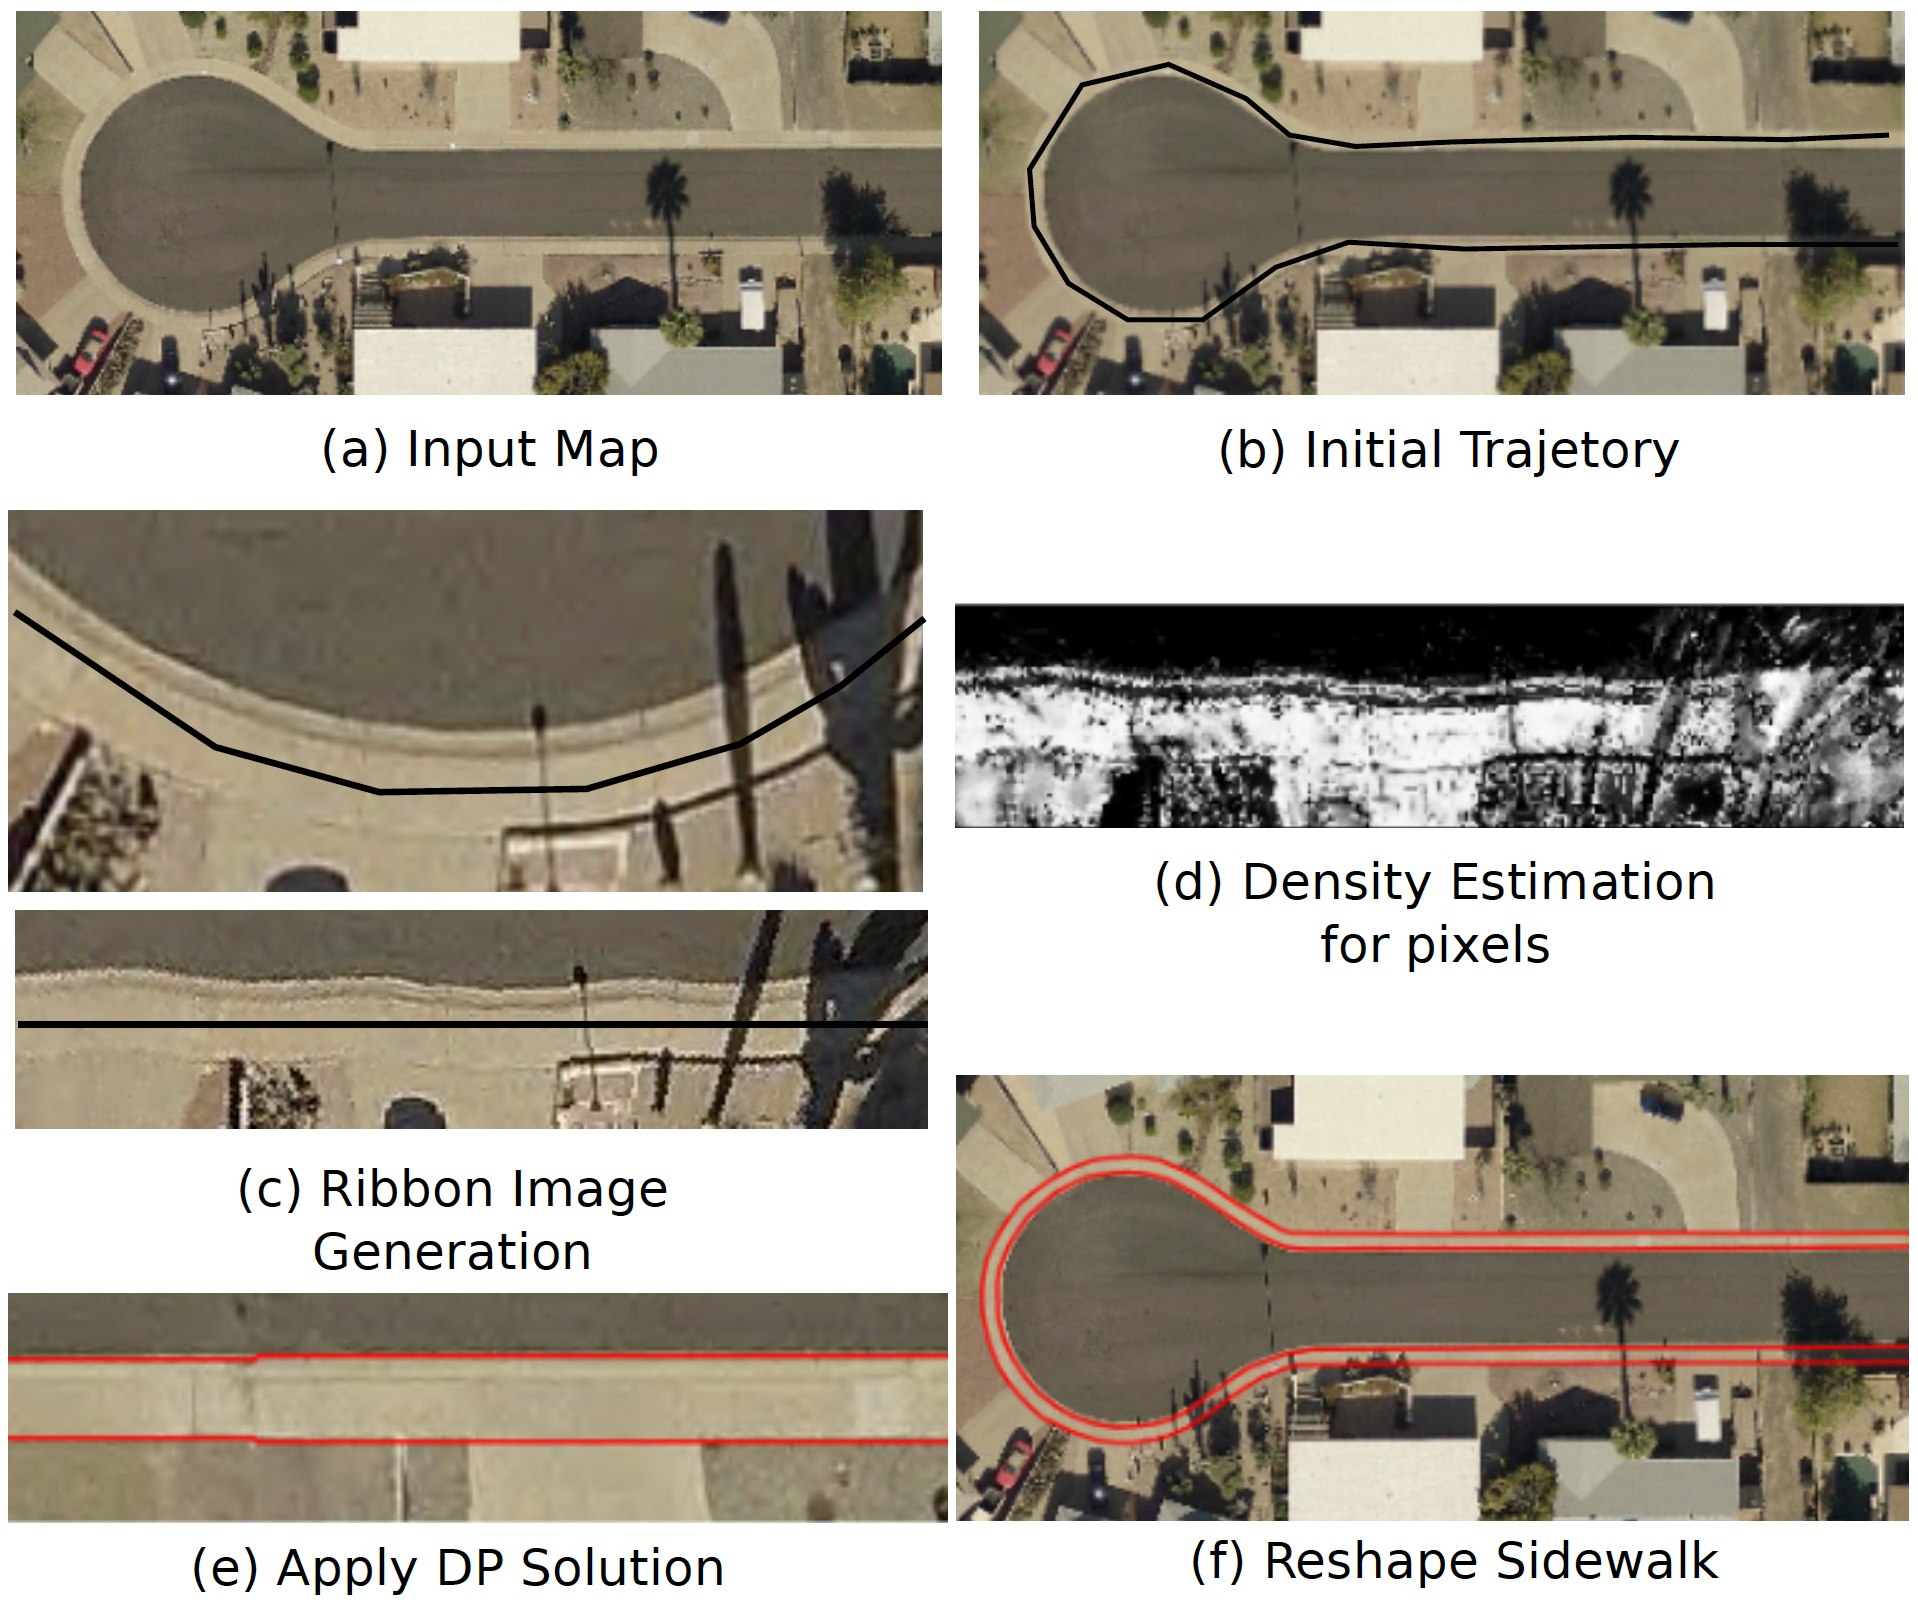
\includegraphics[width=\textwidth]{Figures/diagram.png}
    \caption[Framework Demonstration]{
    Our approach adopted to predict precise boundaries for ribbon-like features. Where black line indicated a sidewalk's geometric information, and red lines shown our result for the sidewalk boundaries. From (a) to (f), the 6 step approach introduce input map (a), initial trajectory (b), ribbon image generation (c), density Estimation for pixels(d), the result from our \ac{DP} solution(e), the result after reshape sidewalk(f).}
    \label{fig:fw_ov}
\end{figure}

\section{Challenges}

\begin{figure}[H]
    \centering
    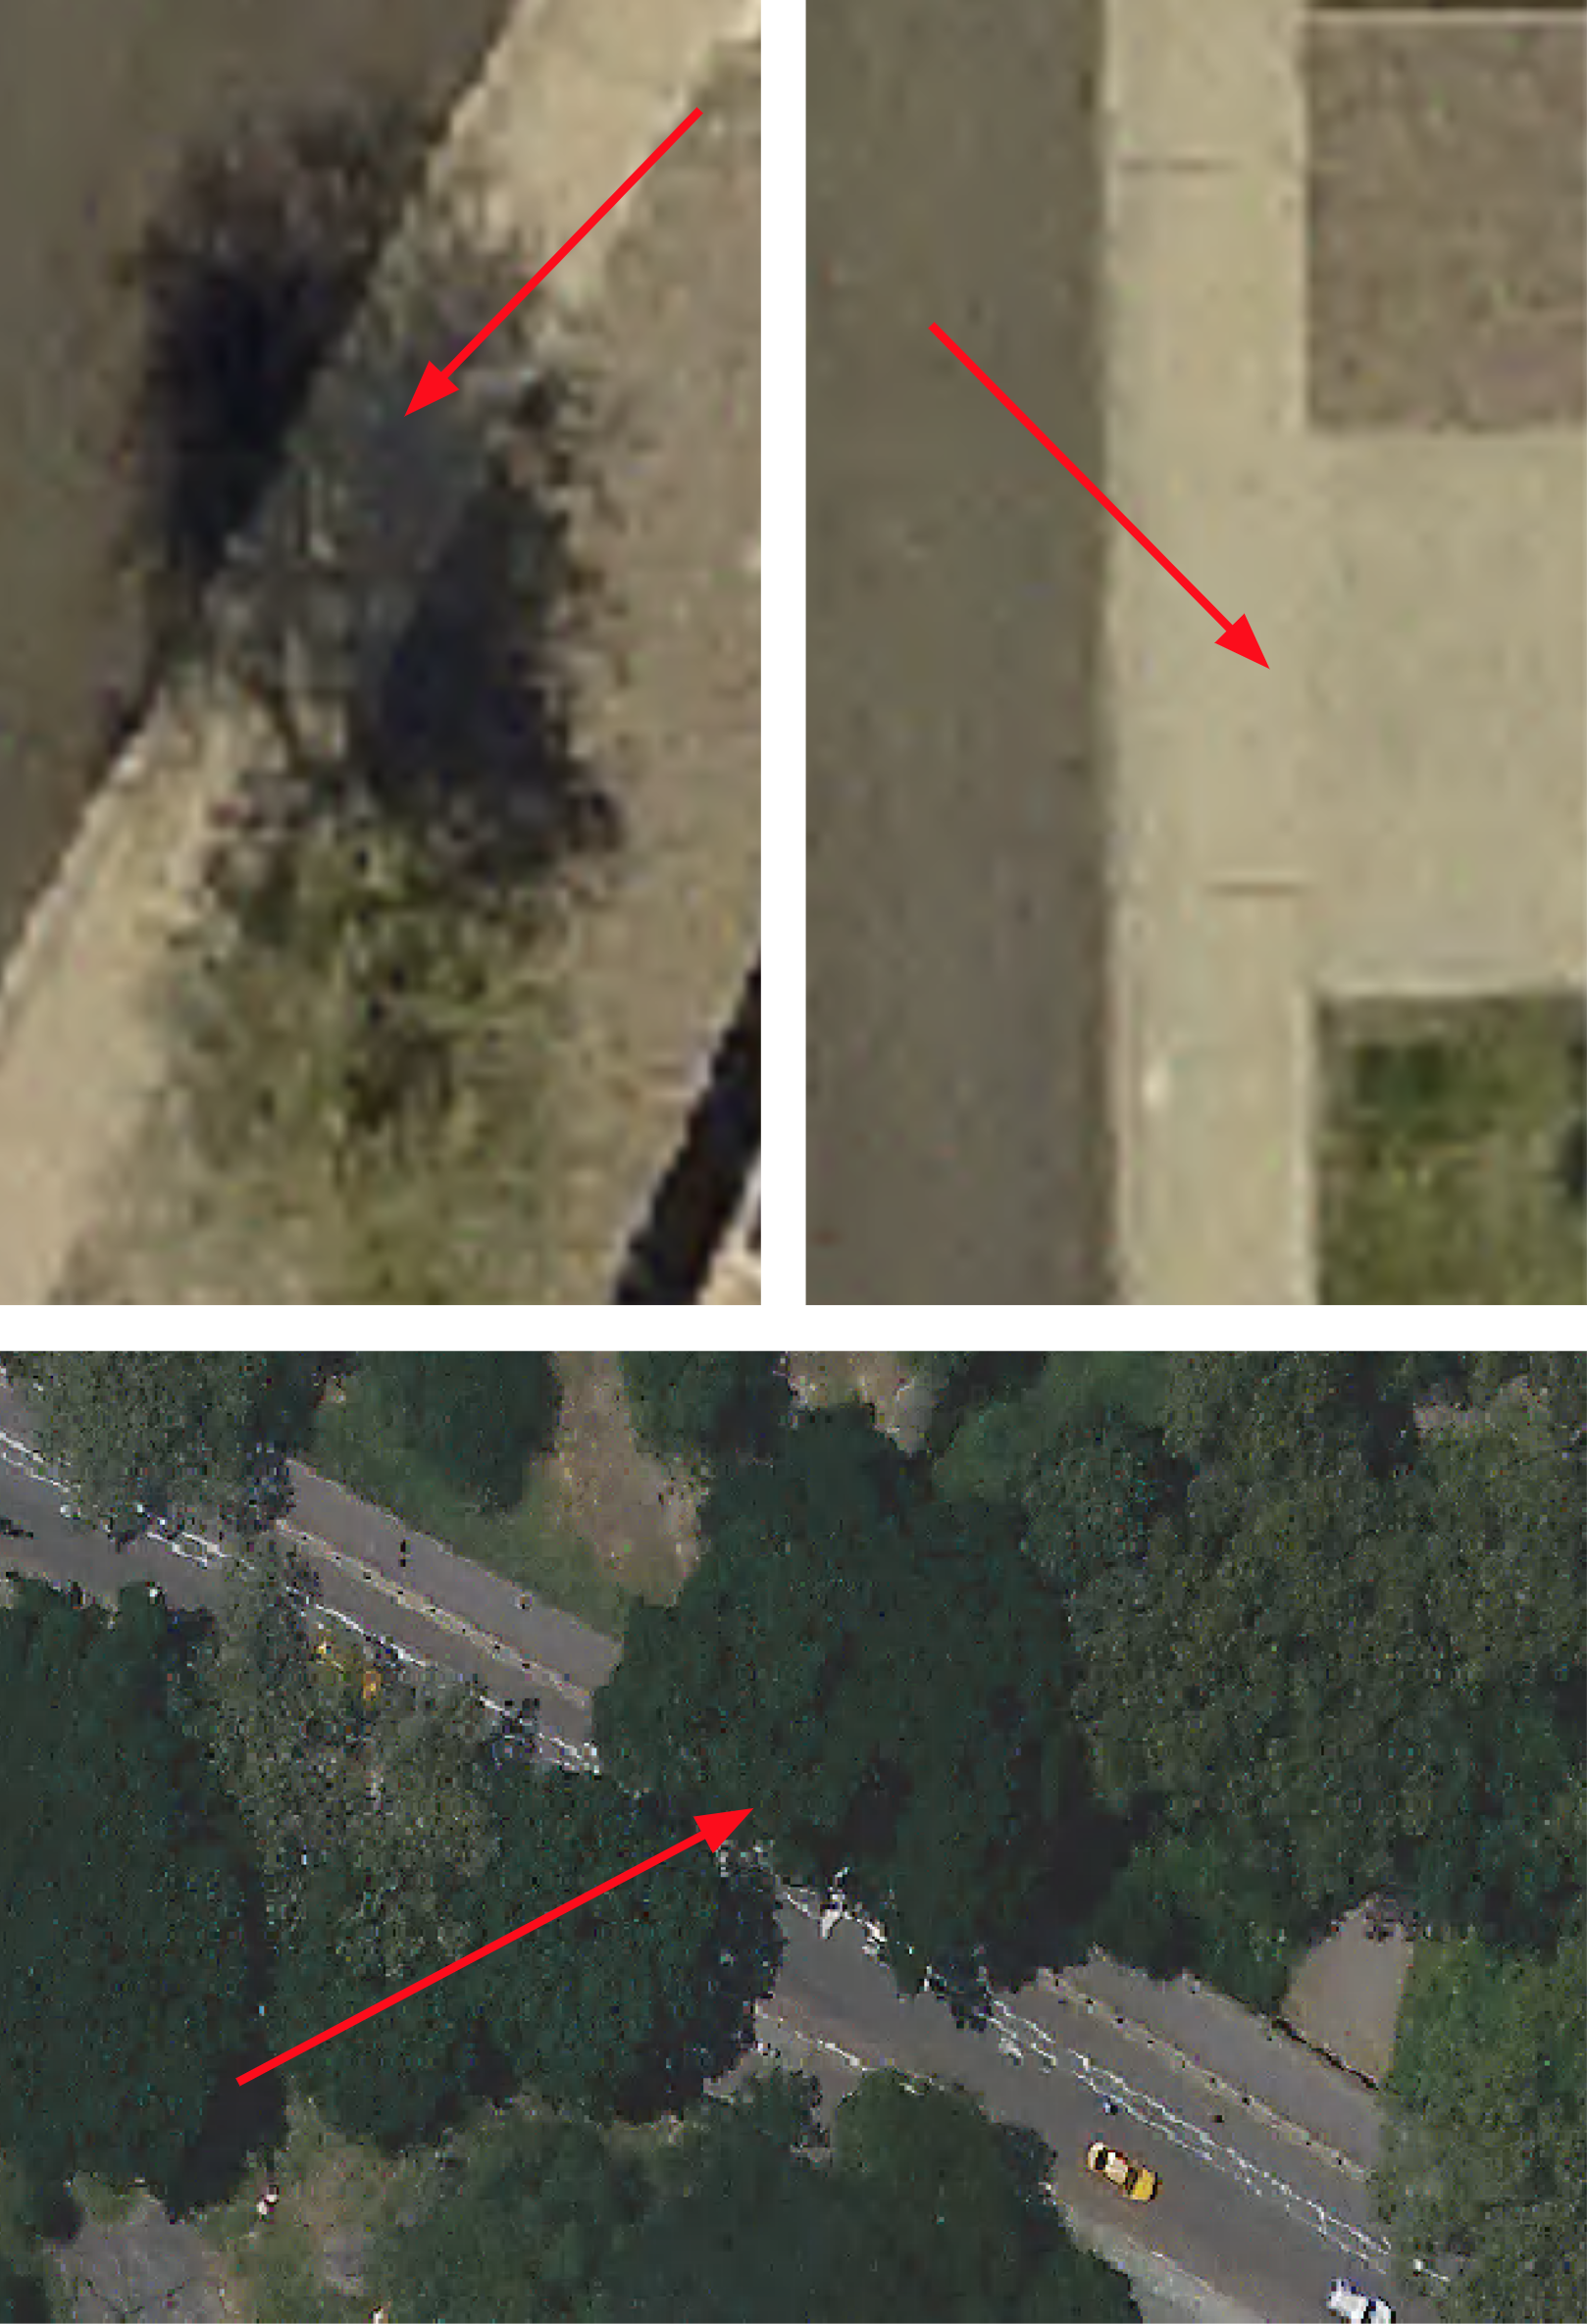
\includegraphics[width=0.75\textwidth]{Figures/Challenge.png}
    \caption[Challenges Demonstration]{A detail demonstrations of challenges that we are facing in our approach. From left to right, top to bottom, it shows that sidewalk are under the shadow, camouflage with adjacent materials and blocked by obstacles.}
    \label{fig:challenge_demo}
\end{figure}

As shown in figure \ref{fig:challenge_demo}, the main challenge addressed by our approach is to predict precise boundaries for ribbon-like walking paths when they are:

\begin{itemize}
    \item blocked by obstacles,
    \item under the shadow of trees, cars, buildings,
    \item camouflage with adjacent materials (e.g. driveways, gutters),
    \item partially damaged so texture varies along the sidewalk.
\end{itemize}

Under the circumstances, most feature segmenting tools will not able to locate accurate boundaries, their results may recognize the non-sidewalk pixels (FP) as the sidewalk or the other way around (FN). 

\section{Contributions}

The aim of this work is to precisely align and determine the width of a coarsely registered ribbon-like feature to match its appearance in a \ac{VHR} image.
The input is a \ac{VHR} georeferenced and orthorectified image along with a set of linear features that are close to, but perhaps not precisely aligned with the center of a ribbon-like feature. 
In particular, we expect that the ribbon will be made of a material with a somewhat uniform appearance (e.g. asphalt, gravel, or concrete) but that its appearance will be affected by shadows and interrupted by occlusions from vegetation, pedestrians, or vehicles such as bicycles. 
Our aim is to determine a more precise mid-line and an estimate for the width of the ribbon-like feature, which can vary slowly along its trajectory. 
The solution proposed in this paper does not rely on prior knowledge of the material on or around the ribbon, but instead, it estimates material appearance as it refines the placement of an initial estimate for the ribbon's mid-line.
	
	Our contributions are as follows:
	\begin{itemize}
		\item A novel \ac{DP} approach is proposed for aligning ribbon-like features to orthoimagery.
		\subitem We do not require large training sets; a few parameters to control the smoothness of the resulting ribbon along with a coarse initial estimate of the trajectory are all that is needed.
		\subitem Unlike methods that aim to recover the trajectories only, in our approach a likely thickness is directly identified so that more plausible trajectories and boundaries can be identified.
		\item An application to the problem of registering sidewalks to aerial photographs is demonstrated, allowing \ac{GIS} data sets to be improved as high-resolution ortho imagery becomes available. 
	\end{itemize}
\chapter{Background}

% To have a better understanding of our approach, it's important to understand the basic concept and assumption that we used to develop the approach. 

\section{\ac{VHR} Aerial Imagery}

\begin{figure}[H]
    \centering
    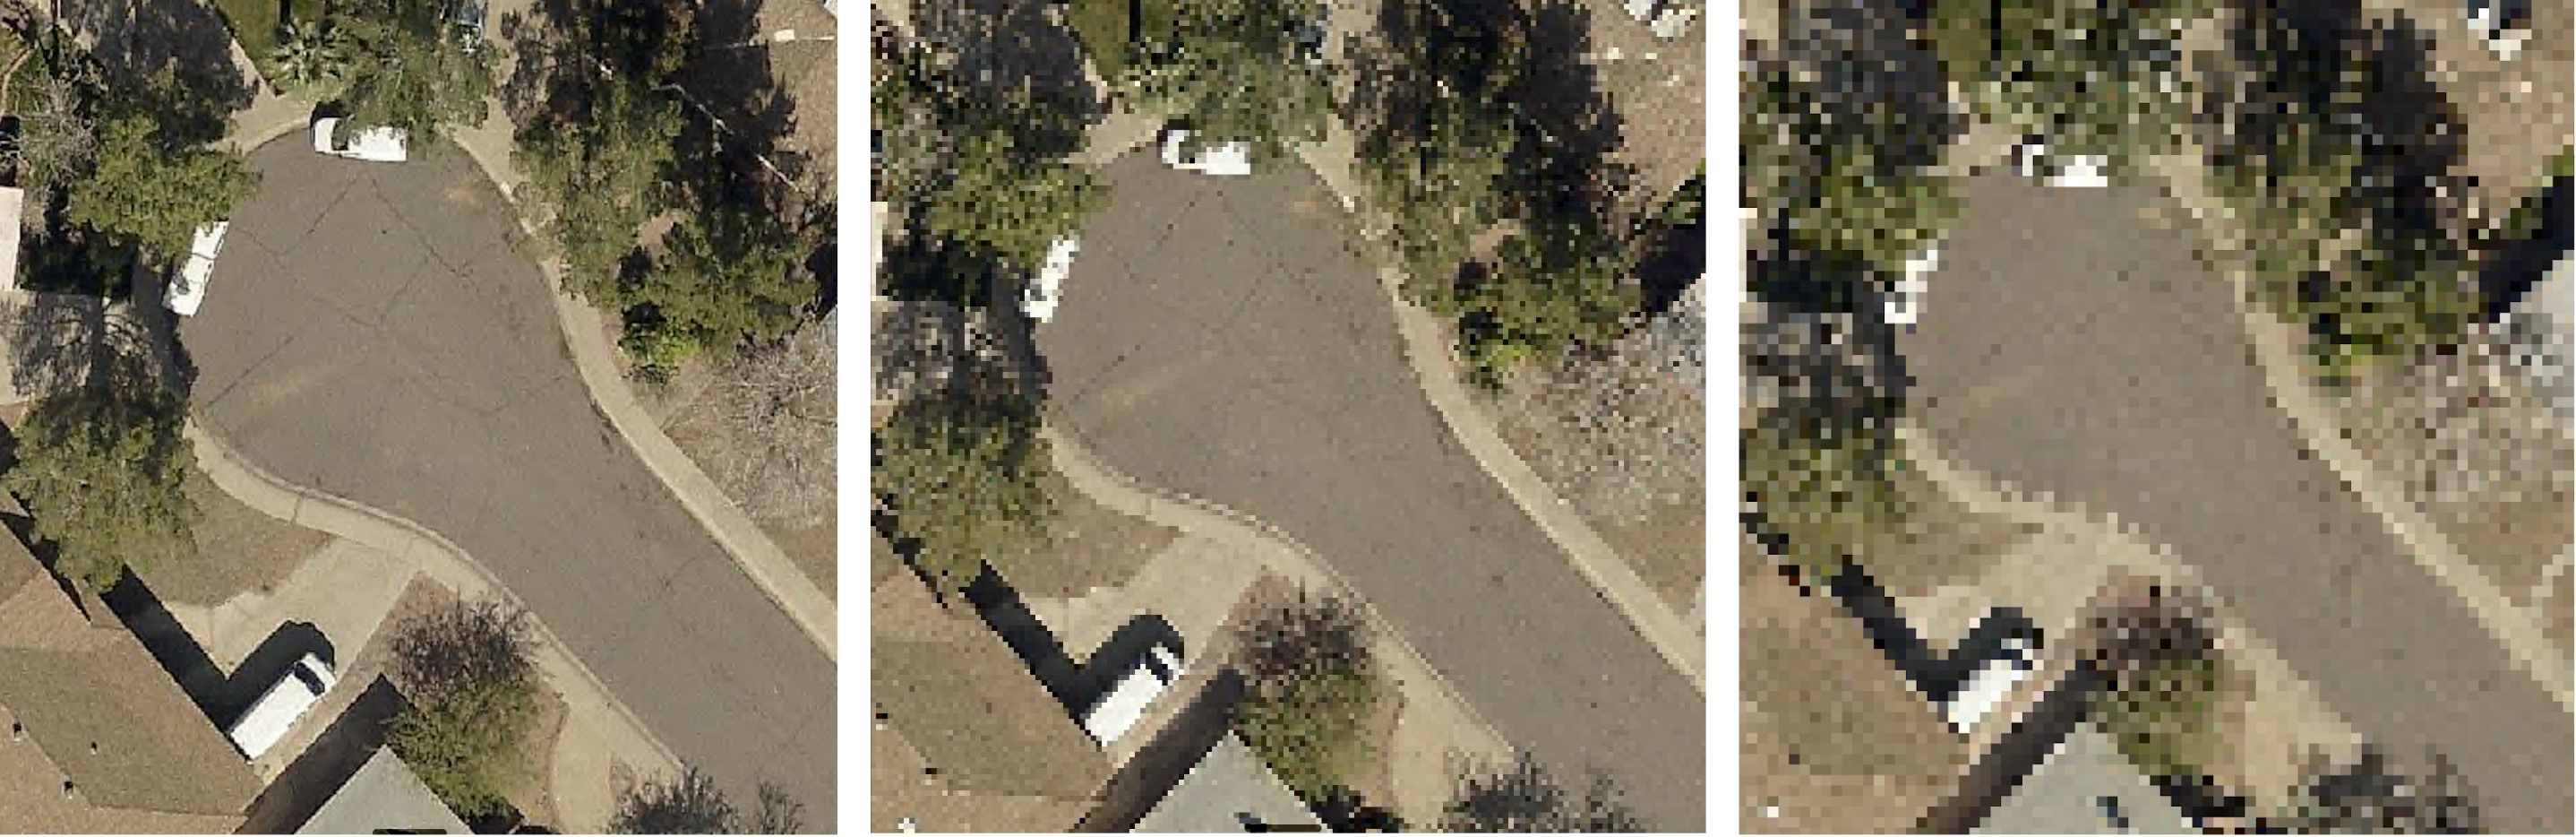
\includegraphics[width=\textwidth]{Figures/arz_7_res_compare.png}
    \caption[Resolution Comparison]{Comparison between different resolutions. From left to right, where (a) has half meter scales, (b) has 5 meter scales and (c) has 10 meter scales. With the increase of meter scale, it harder to capture the boundary of the edges detail of sidewalks.}
    \label{fig:vhr_compare}
\end{figure}
% \todo{change dpi to 5 meter scale. make it worse.}

\ac{VHR} stands for Very High Resolution, it has advantageous for buildings extraction, road detection or image segmentation~\cite{FREIRE20141, 10.1007/BFb0015525, 10.1007/978-3-642-15567-3_16}. 
These aerial imageries contain more information and detail due to the higher resolution, which give us the ability to develop more complex analysis on the imagery with same size.
\figref{fig:vhr_compare} demonstrates the difference between different resolution within the same area. From (a) to (c), the resolution changes from half meter scale to 10 meter scale. 
With higher resolution, it's easier to find the precious boundaries of an object or identify it. 
For building extraction, higher resolution provides more information when dealing with complex houses or extract complex suburban roofs~\cite{10.1007/BFb0015525}. 
For thin ribbon-features segmentation such as sidewalks in our approach, to visualize an overlaid map without high resolution, the imagery can be distracting, and the output may effect by tiny discrepancies between digitized pathways~\cite{10.1007/978-3-642-15567-3_16}. 

\section{\ac{OSM}}
\begin{figure}[H]
    \centering
    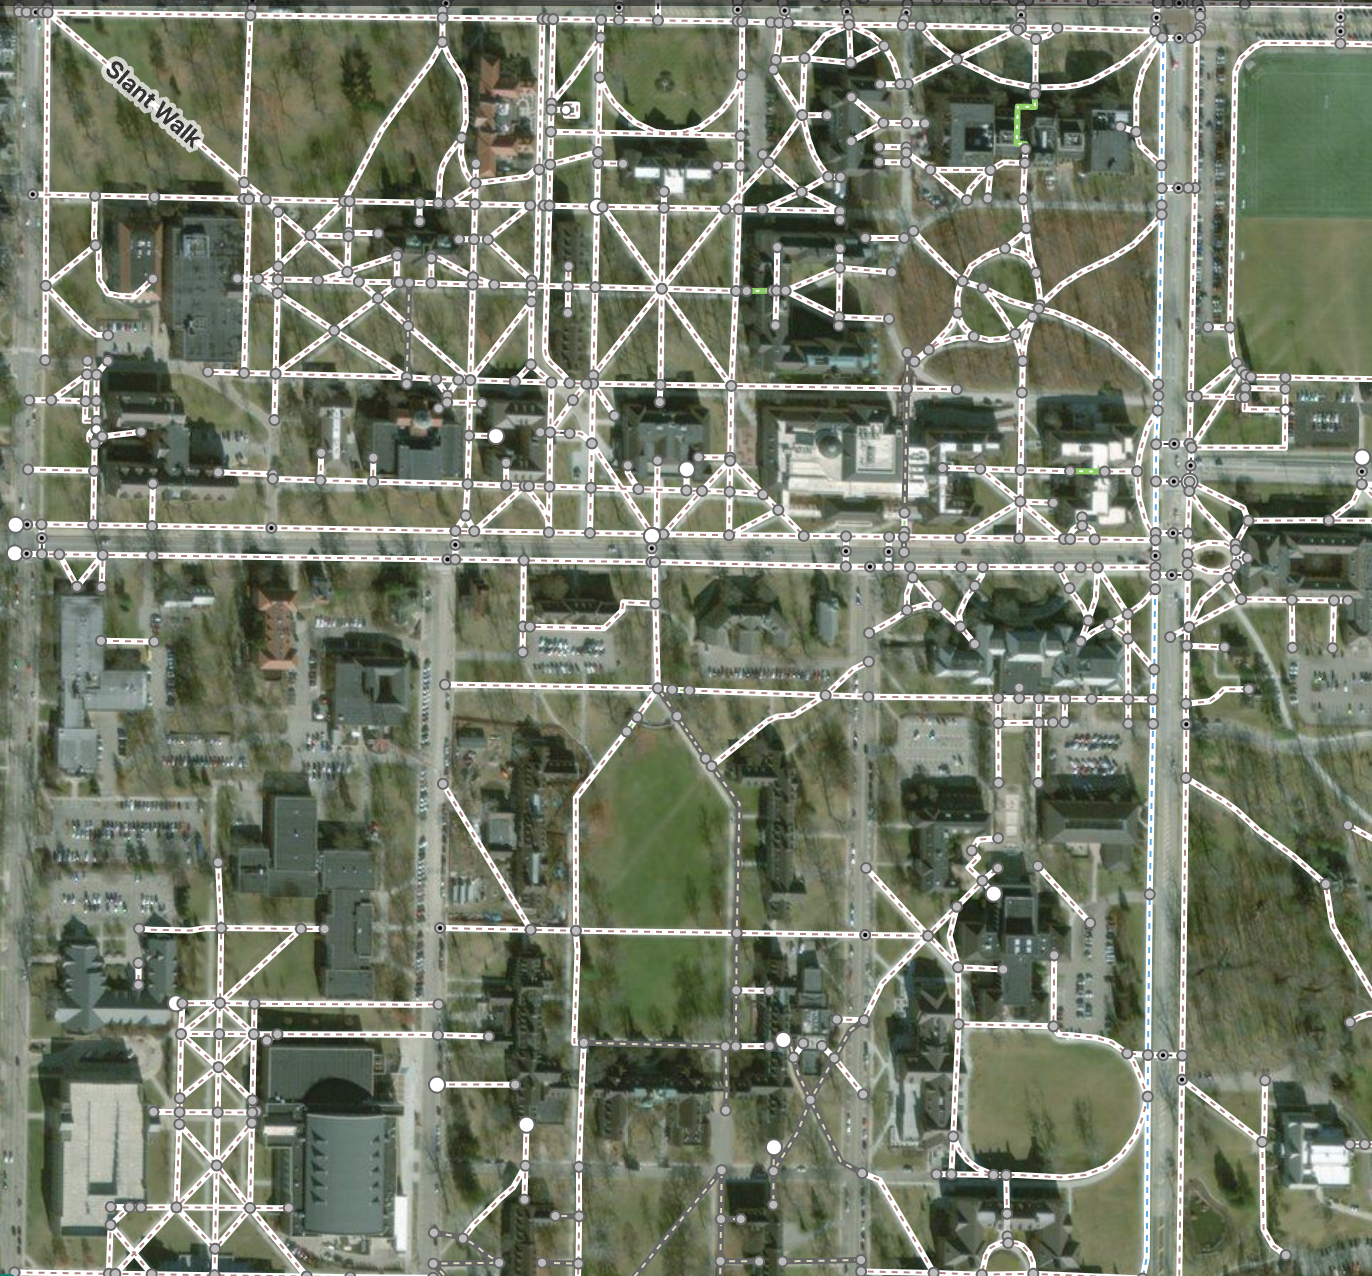
\includegraphics[width=0.85\textwidth]{Figures/oxford_path_data_osm.png}
    \caption[\ac{OSM} Walking Path]{A demonstration of actual walking path data from \ac{OSM}. The figure shows in the Oxford area in Ohio, US. Row 2 specifies the zoom in version of error that we need to facing. The sidewalk misses in the path data (left), the path data marks offset compare to the actual sidewalk(right).}
    \cite{OpenStreetMap}
    \label{fig:osm_oxford_path}
\end{figure}

\ac{OSM} stands for Open Street Map, which was founded by Steve Coast in 2004~\cite{lasPiñas, OpenStreetMap}. 
\ac{OSM} is a collaborative project that allows users to generate a free editable map of the world~\cite{4653466}.
Rather than the map itself, \ac{OSM} generates the data with the map information that across most of the world as primary output. 
It also allows users to develop the map data with portable satellite navigation devices. 
With all these convenience features, \ac{OSM} is helpful for the map analysis and features segmentation~\cite{10.1007/11744078_9}. 
\figref{fig:osm_oxford_path} shows that \ac{OSM} supports features like footpaths, roads, buildings, and others, with the ability to extract the \ac{GIS} data for any individual feature. 
It may also leads to the issue of dealing with missing or invalid data when we rely on the data set for auto-detection, or mismatch data with imagery when structures changes along with time.

\section{\ac{CRF}}
\ac{CRF} stands for Conditional Random Field, which is a class of statistical modeling method that often applied in pattern recognition and machine learning~\cite{MAL-013}. 
As a type of discriminative undirected probabilistic graphical model, \ac{CRF} is commonly used for segmenting, labeling or parsing of sequential data, such as in computer vision, structure segmentation and object recognition~\cite{RuizSarmiento2015UPGMppA, 1315232, lafferty2001conditional}. 
For road segmentation, several approaches are able to locate the precise boundaries by treating it as a \ac{CRF} problem~\cite{ActiveContou09, Achanta:149300}. 

\section{\ac{GMM}}

\ac{GMM} stands for Gaussian Mixture Models~\cite{sridharan2014gaussian}.
It is a probabilistic model for representing normally distributed subpopulations within an overall population.
\ac{GMM} often can be performed when the data points are mixtures of a Gaussian distribution. 
It can be used in common computer vision tasks such as background and foreground subtraction~\cite{1333992}. 
For road segmentation, we can treat the problem as subtract foreground (road feature) from the complex background (non-road feature). 
\figref{fig:gmm_sample_1} demonstrate the comparison between foreground and background \ac{GMM} on sample walking path show in gray-scale. 
For foreground subtraction, which shown in row 1 and row 3, we treat sidewalk texture as foreground and apply the \ac{GMM} algorithm to subtract it from the background (non-sidewalk texture). 
Background subtraction are shown in row 2 and row 4, we did the opposite and treat non-sidewalk part as foreground. 

\begin{figure}[H]
    \centering
    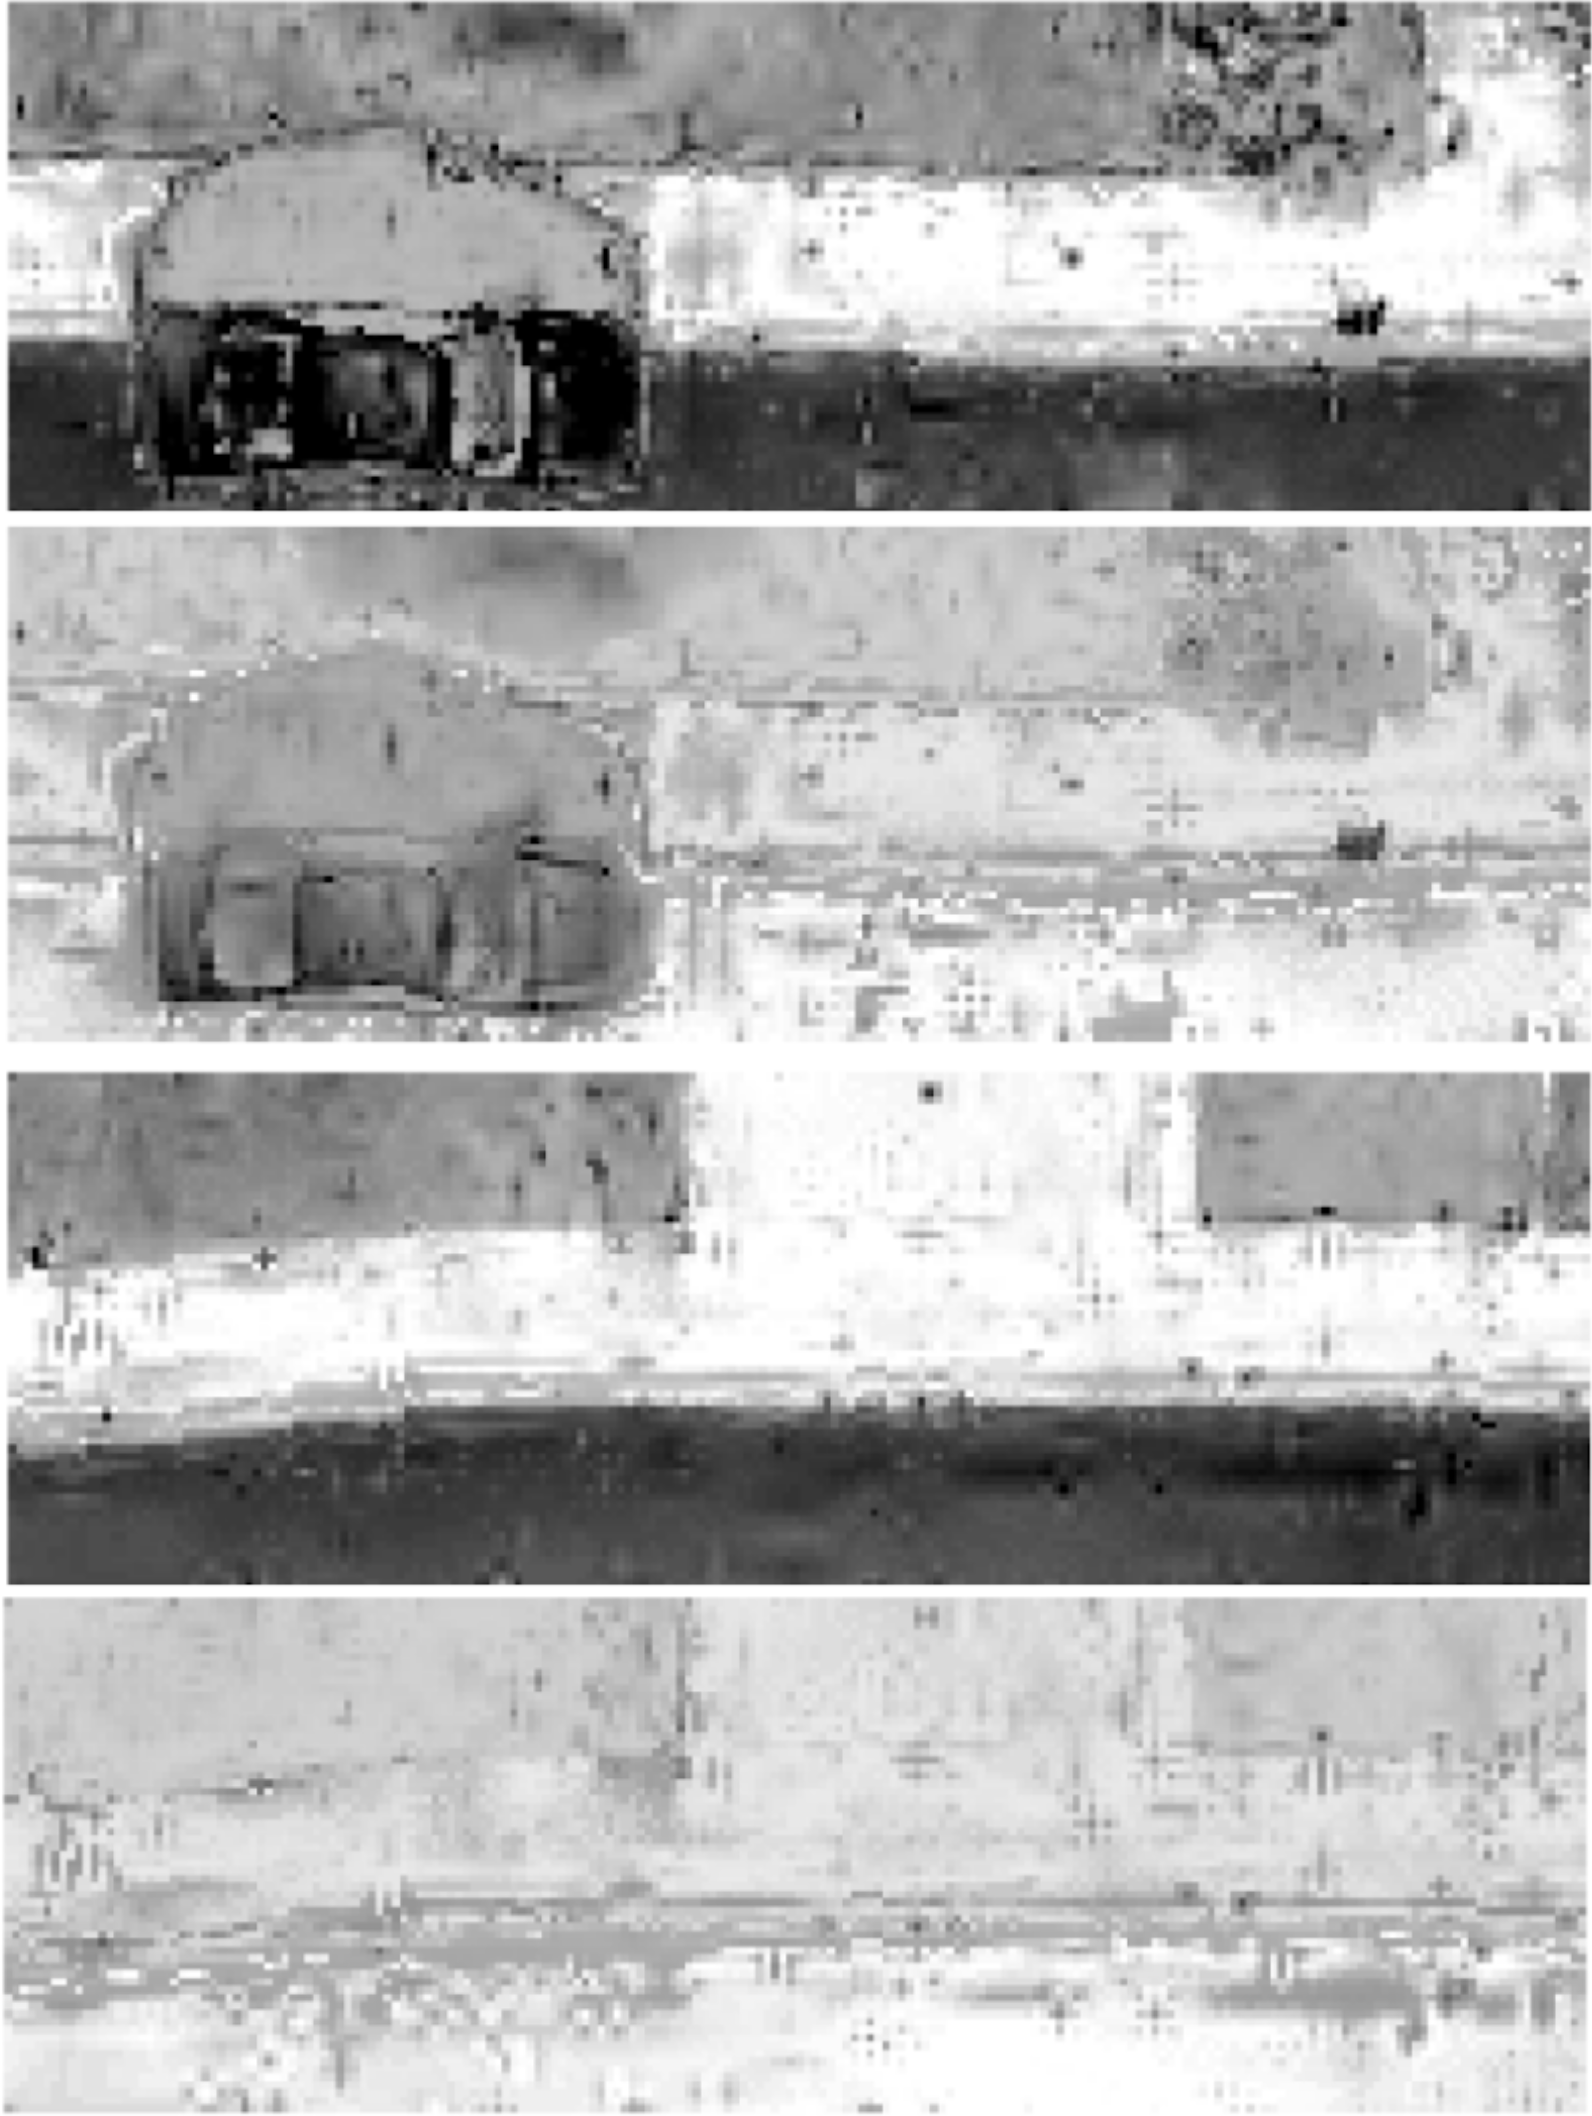
\includegraphics[width=0.85\textwidth]{Figures/GMM_needed.png}
    \caption[Density Background Subtraction]{A demonstration of apply \ac{GMM} algorithm on sample inputs, show with gray scale. From top to bottom, row 1 shows foreground density on sample path, row 2 show background density on the same sample path as row 1. Same with row 3 and 4, with different sample path. For foreground density, lighter color represent more likely to be sidewalk and darker color represent more likely to be non-sidewalk. Background density shows as the opposite.}
    \label{fig:gmm_sample_1}
\end{figure}


\section{\ac{DP}}
\begin{figure}
    \centering
    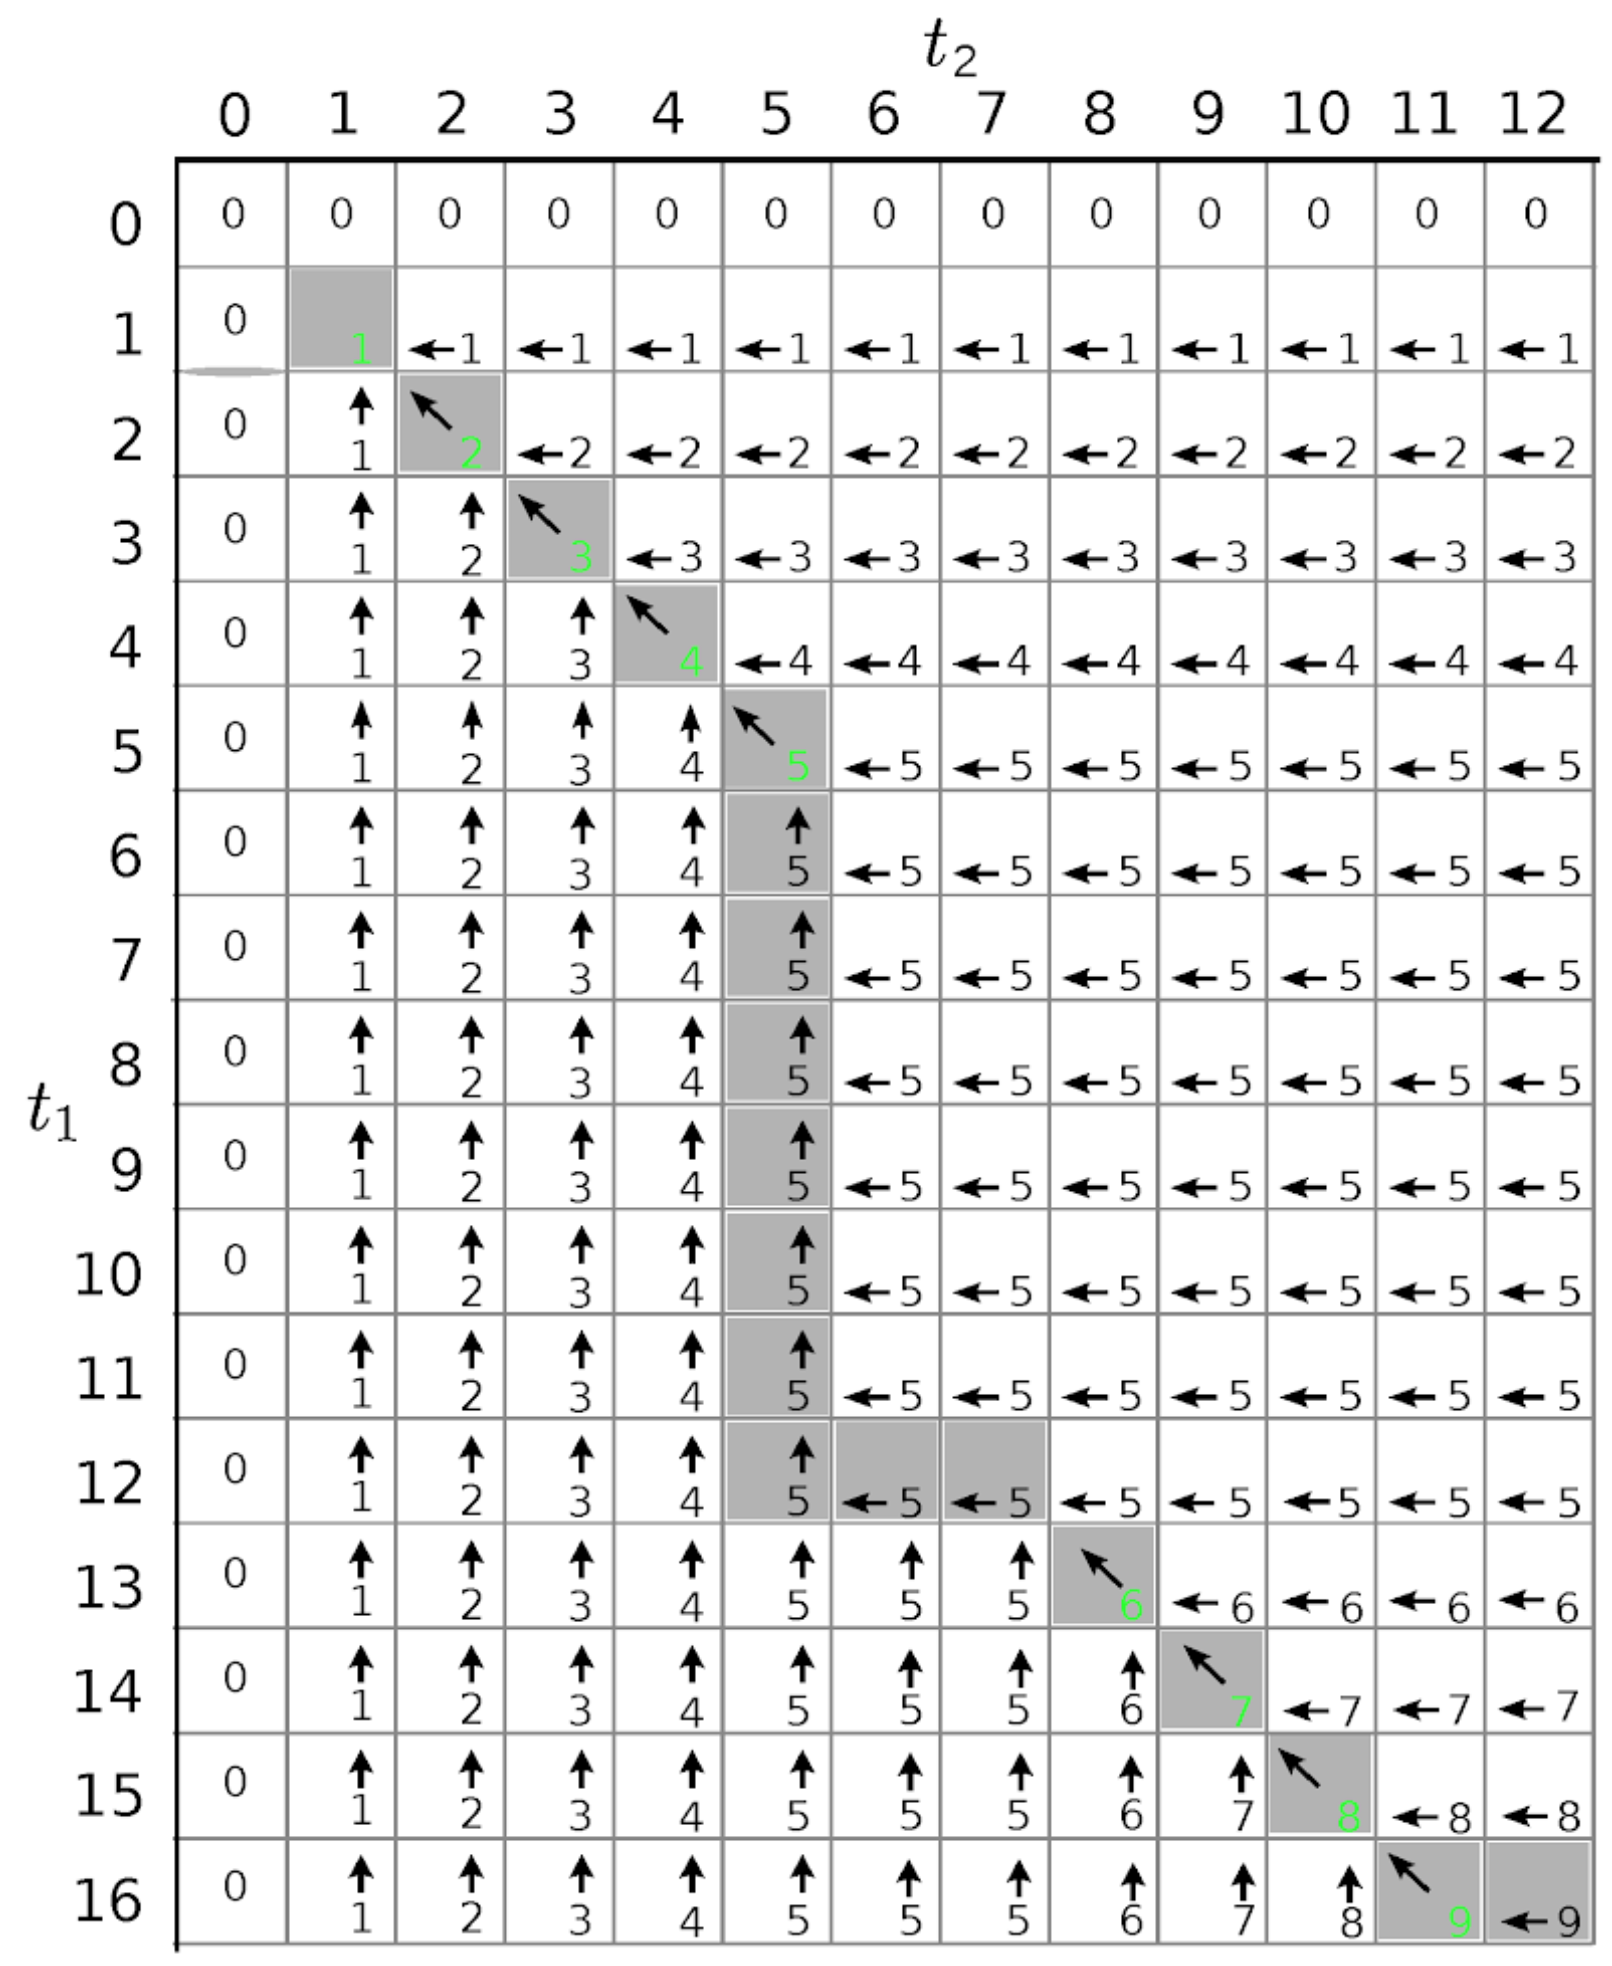
\includegraphics[width=0.9\textwidth]{Figures/longest_common_sequence.png}
    \caption[Demonstration on Longest Common Sequence]{Dynamic Programming demonstration with longest common sequence. Similar to our approach, to find the longest common sequence, it first needs to fill the table with \ac{DP} and then backtrack to find the longest path. It used in intersection detection with GPS trace~\cite{Xie2017DetectingRI}.
    }
    \label{fig:lcs_dp}
\end{figure}

\ac{DP} stands for Dynamic Programming. It is both a mathematical optimization method and a computer programming method \cite{bertsekas2005dynamic}. 
In 1950s \ac{DP} was invented by Richard Bellman\cite{bellman2013dynamic}. 
The main concept of \ac{DP} is to simplify a complicated problem by breaking it down into simpler sub-problems in a recursive manner \cite{howard1966dynamic}. 
In computer science, if a problem can break into serial sub-problems and each sub-problem can be recursively solved by finding its optimal solution, then we know that \ac{DP} are applicable. 

\figref{fig:lcs_dp} gives a example of a famous dynamic programming problem, Longest Common Sequence. To achieve the result of finding the longest common sequence, it first needs to fill the table with \ac{DP} and then backtrack to find the longest path. One method gives approach with using longest common sequence for intersection detection from GPS traces~\cite{Xie2017DetectingRI}.

Dynamic Programming has a variety of applications since it can significantly reduce the run-time \cite{bertsekas1995neuro}. 
We use Fibonacci Sequence to demonstrate the \ac{DP} process\cite{horadam1961generalized}. 
Figure \ref{fig:fbs}, row 1 shows that to calculate the $n^{th}$ Fibonacci number, it require a certain exponential rate of calculation to finish the process.
The time complexity can be reduced since it is re-calculating the previous Fibonacci number repeatedly. 
By applying \ac{DP} algorithm, we can save the previous calculated Fibonacci number and reused it when needed.
Figure \ref{fig:fbs}, row 2 indicate the same process after applying dynamic programming, we marked unnecessary steps in red X. 
By trade in linear space to save previous calculation, we can reduce the wrong time from exponential to linear.

\begin{figure}[H]
    \centering
    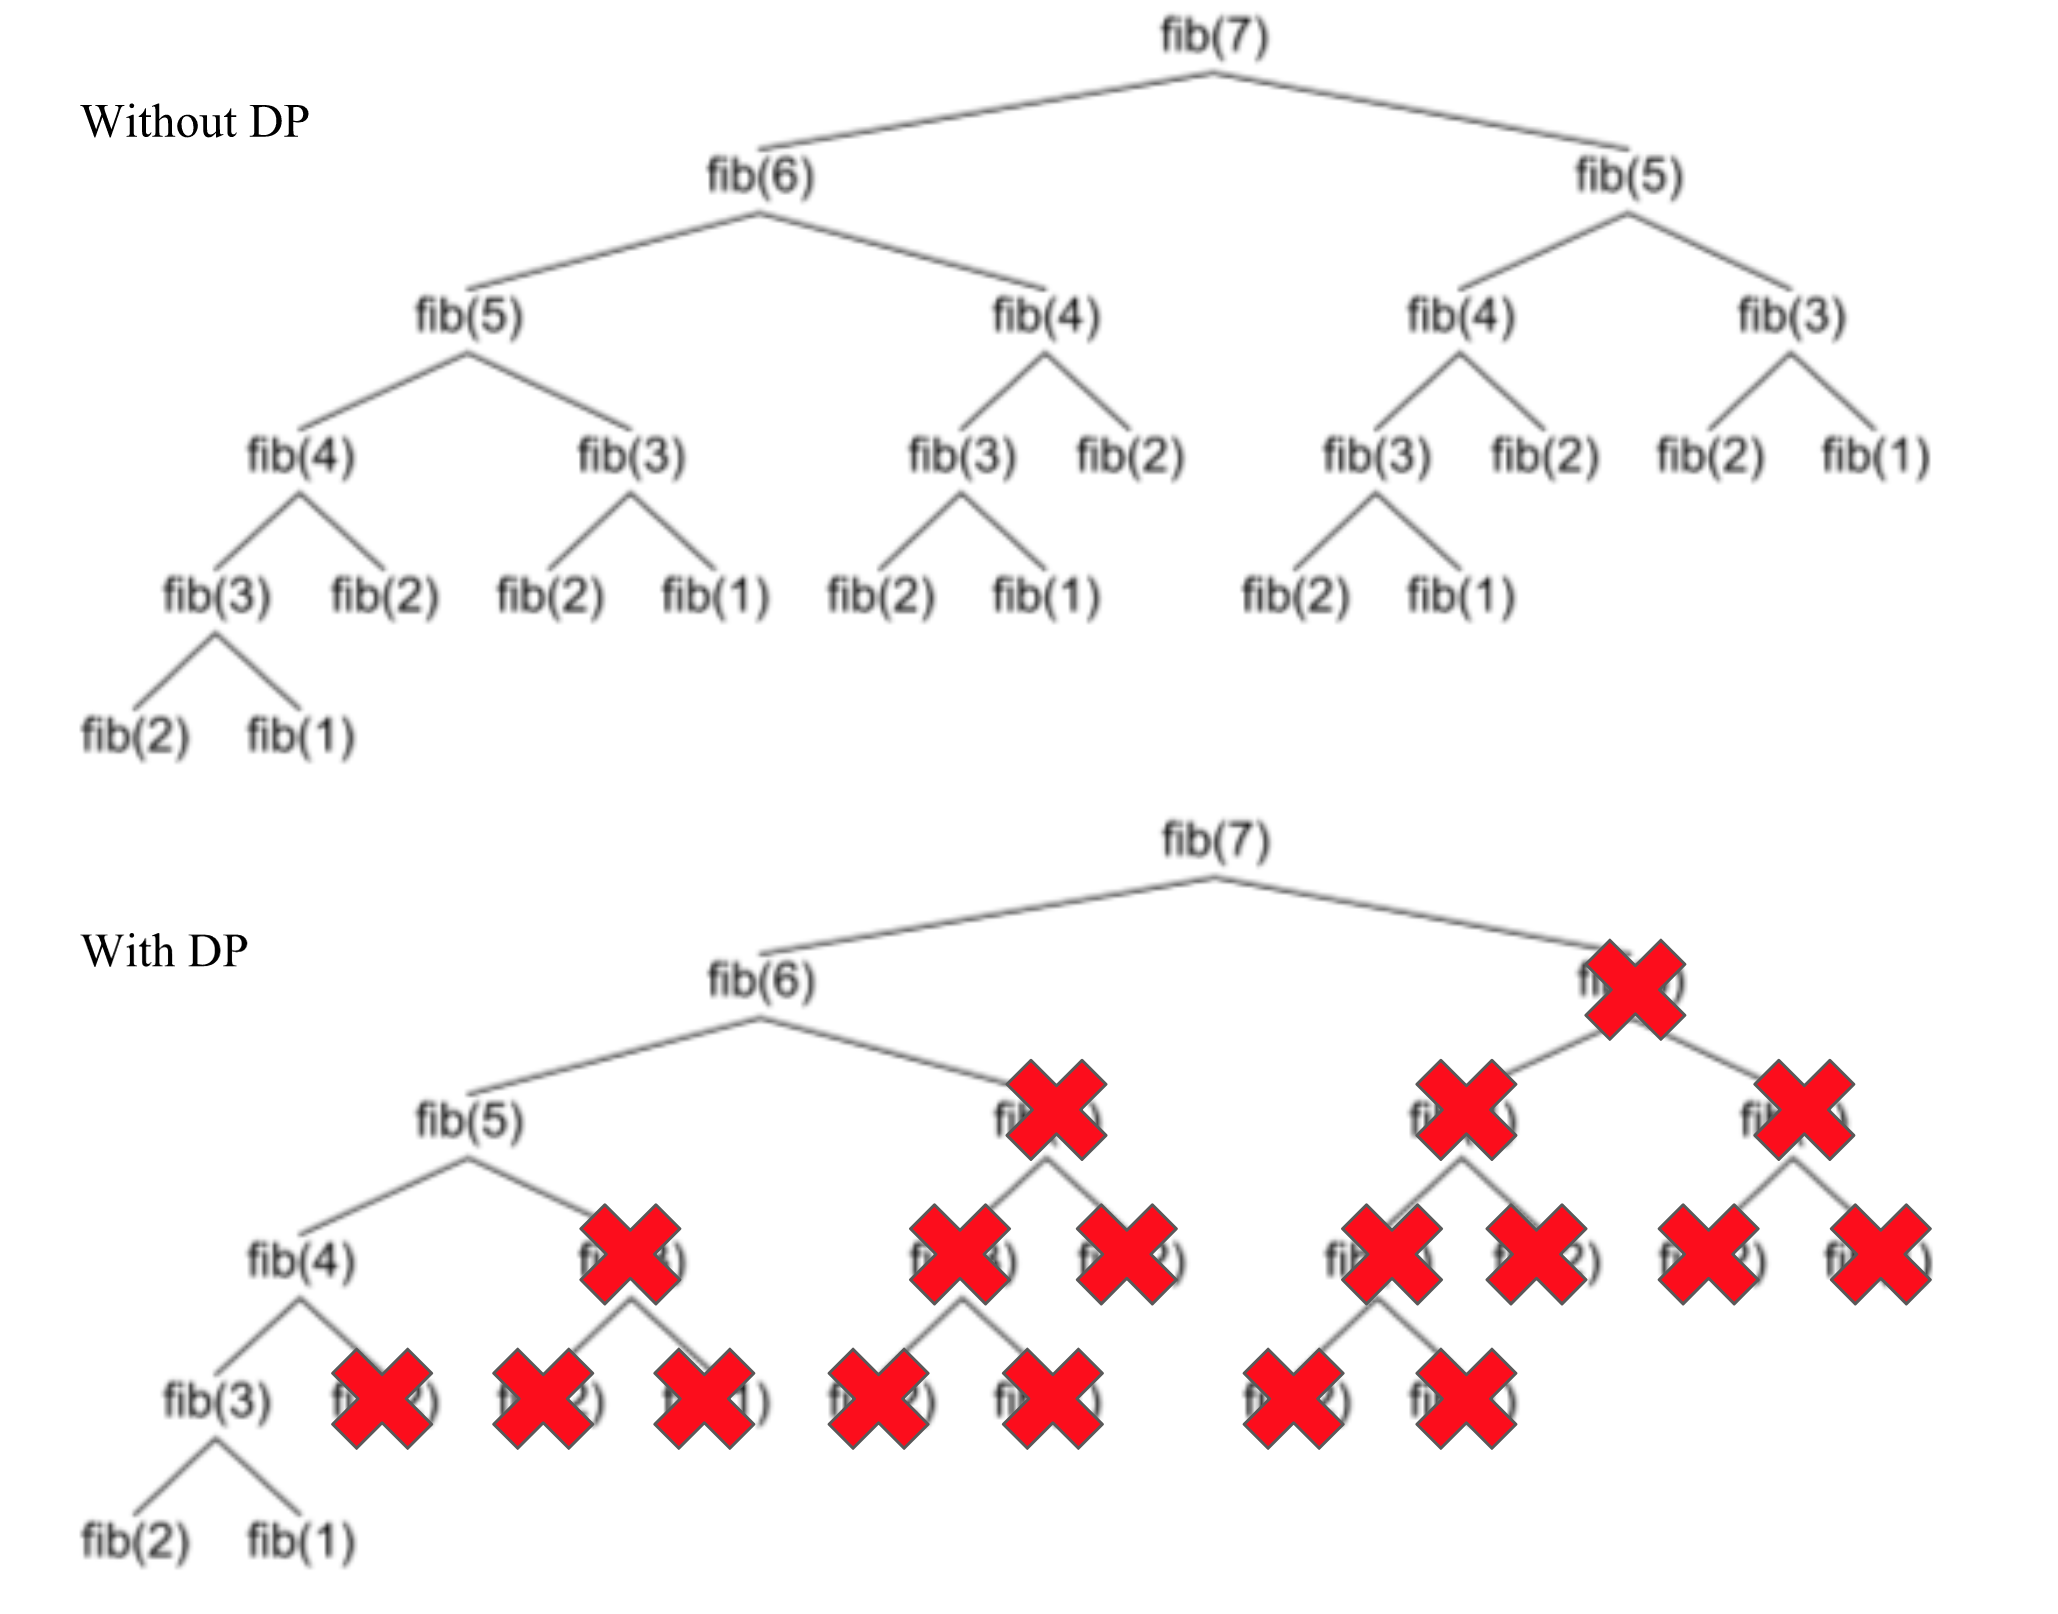
\includegraphics[width=\textwidth]{Figures/treewithdp.png}
    \caption[Demonstration on Fibonacci Sequence]{Representing the calculation of Fibonacci Sequence ($7^{th}$) with binary tree. Row 1 shows without applying dynamic programming, it need's certain exponential rate to calculate $n^{th}$ Fibonacci number. With the increase of $n$, the number of calculation increase significantly. Row 2 shows with dynamic programming, after saving previous calculation, it's only require linear time steps to calculate $n^{th}$ Fibonacci number. We marked unnecessary steps in red X to show it's can be skipped. }
    % \cite{stack_overflow}
    \label{fig:fbs}
\end{figure}

% \begin{figure}
%     \centering
%     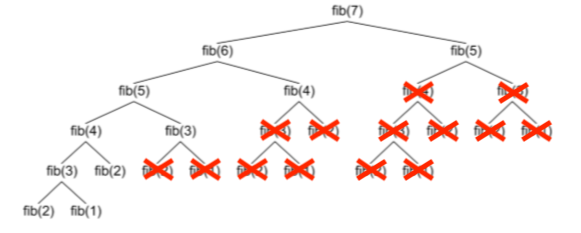
\includegraphics[width=\textwidth]{Figures/QVSdv_DP.png}
%     \caption[Demonstration on Fibonacci Sequence with \ac{DP}]{Representing the calculation of Fibonacci Sequence ($7^{th}$) with binary tree. With dynamic programming, after saving previous calculation, it's only require linear time steps to calculate $n^{th}$ Fibonacci number. We marked unnecessary steps in red X to show it's can be skipped.
%     }
%     % \cite{stack_overflow}
%     \label{fig:fbs_dp}
% \end{figure}

% \section{Street Network Extraction}
% boss paper, 2018 cvpr, they don't gurant to find the center of road.


\chapter{Related Work}

A variety of approaches are able to locate precise object boundaries, although few directly address the problem of sidewalk segmentation in "blobby" or compact regions. Several tools for segmentation appear for segmenting ribbon-like features in \ac{VHR}, we list Grabcut \cite{Rother2004-ou}, Slic\cite{Achanta:149300}, and Active Contours \cite{Kass88snakes:active} as examples.
Results for these methods on a simple sidewalk are shown in \figref{fig:Method_comparison} which shows qualitative results of each method. We observe that grabcut had decent performance on this example, but it is still unable to identify edges in shadow or correctly determine the width of the sidewalk region in the vicinity of a driveway, which seems to be made of the same material as the sidewalk. In addition we observe that all three approaches recognize the gutter as part of the sidewalk because it has the similar texture.  
\begin{figure}[H]
    \centering
    \includegraphics[width=0.55\textwidth]{Figures/compare.png}
    \caption[Method comparison with Grabcut, Active Contours, and Slic]{
        % Method comparison with Grabcut, Active contour and Slic
        A comparison between Grabcut(left), SLIC (center) and Active Contours (right) 
        on an example of a sidewalk from 6-inch aerial imagery; 
        \aclp{TP} are rendered in green, 
        \aclp{FN} are rendered in blue, and 
        \aclp{FP} are rendered in red.
        The SLIC image contains all super-pixels that intersect the initial trajectory of a walking path; the Active Contours and GrabCut methods are initialized with the SLIC results.
    }
    \label{fig:Method_comparison}
\end{figure}

\section{Image Segmentation via Grabcut} 

\begin{figure}[H]
    \centering
    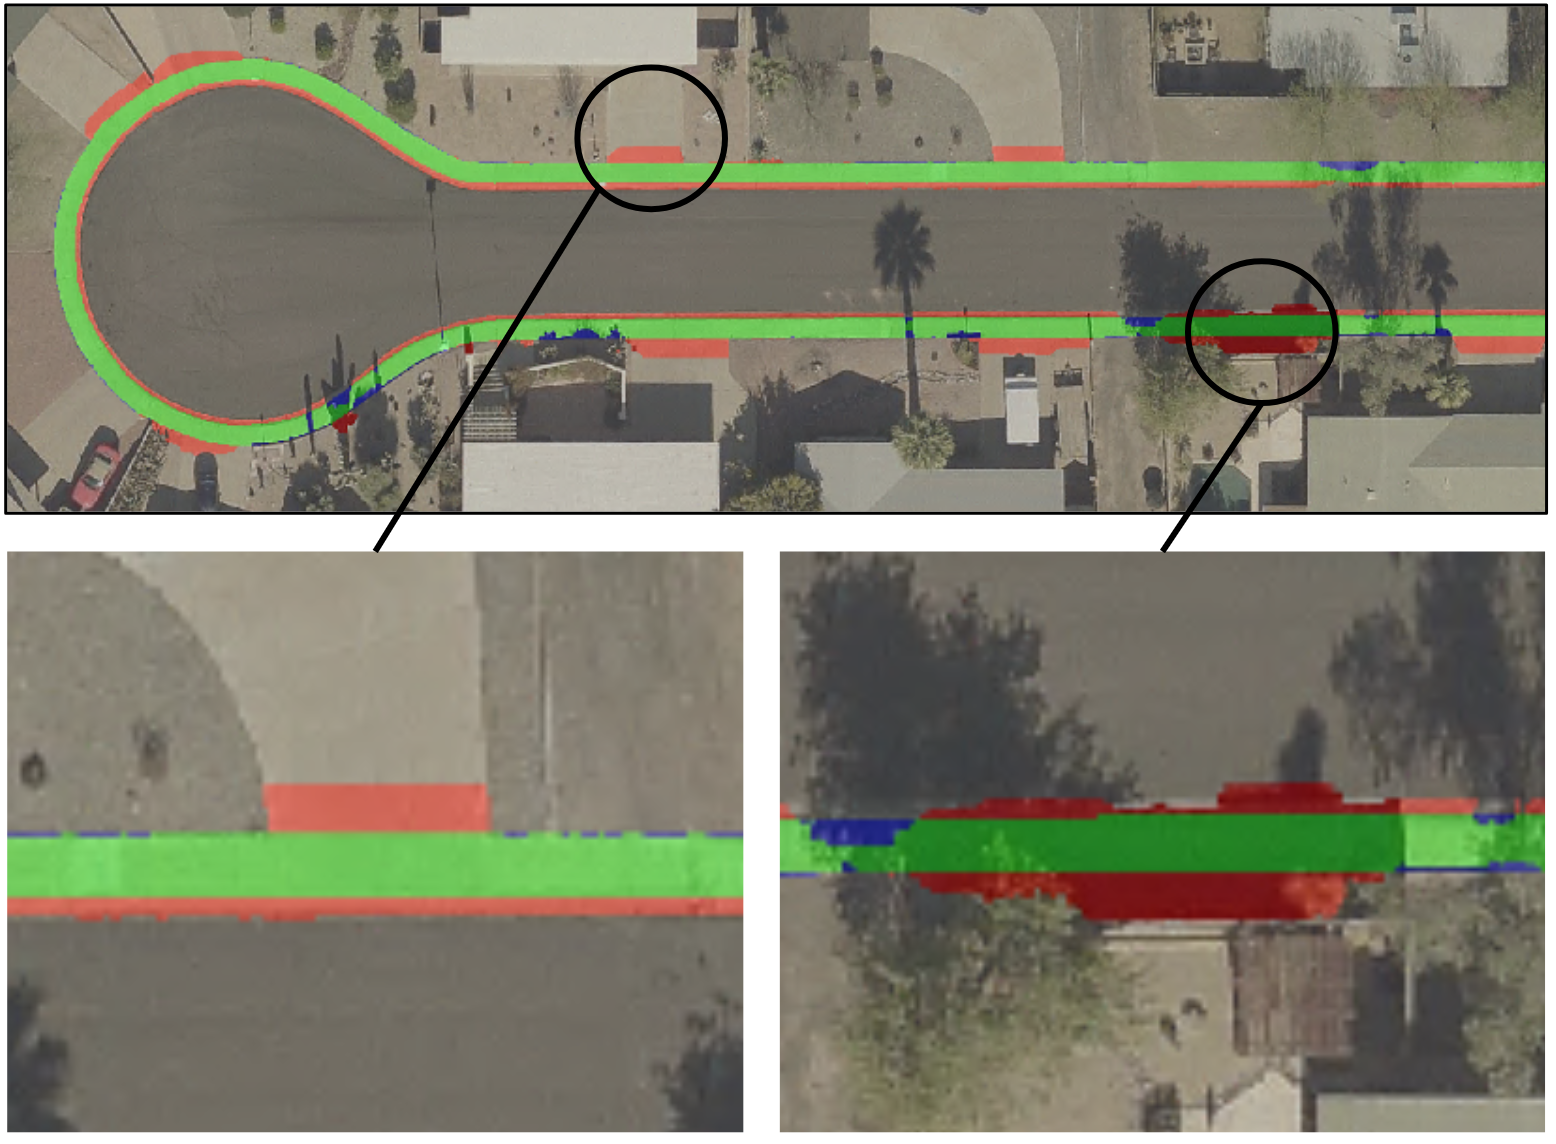
\includegraphics[width=\textwidth]{Figures/grabcut_sample.png}
    \caption[Example of Grabcut]{Detail demonstration with grabcut method. Row 2 indicates examples of false positive, which is recognized a non-sidewalk feature (shadow) and similar texture (driveway) as a part of sidewalk.}
    \label{fig:grabcut}
\end{figure}

Grabcut is a powerful image segmentation tool that combines both texture(color) and edge(contrast) information \cite{Rother2004-ou}. It was designed to efficiently extract a foreground object from a complex background. According to figure \ref{fig:Method_comparison} and figure \ref{fig:grabcut}, the overall performance on grabcut applied to a ribbon-like feature is fairly accurate, but it's hard to identify objects above the sidewalk such as shadows, gutters or foliage. Grabcut seems to identify the occluded regions as negative, we suspect that is because of the lack of width control.

\section {Super-pixels and Feature Extraction with SLIC}

\begin{figure}[H]
    \centering
    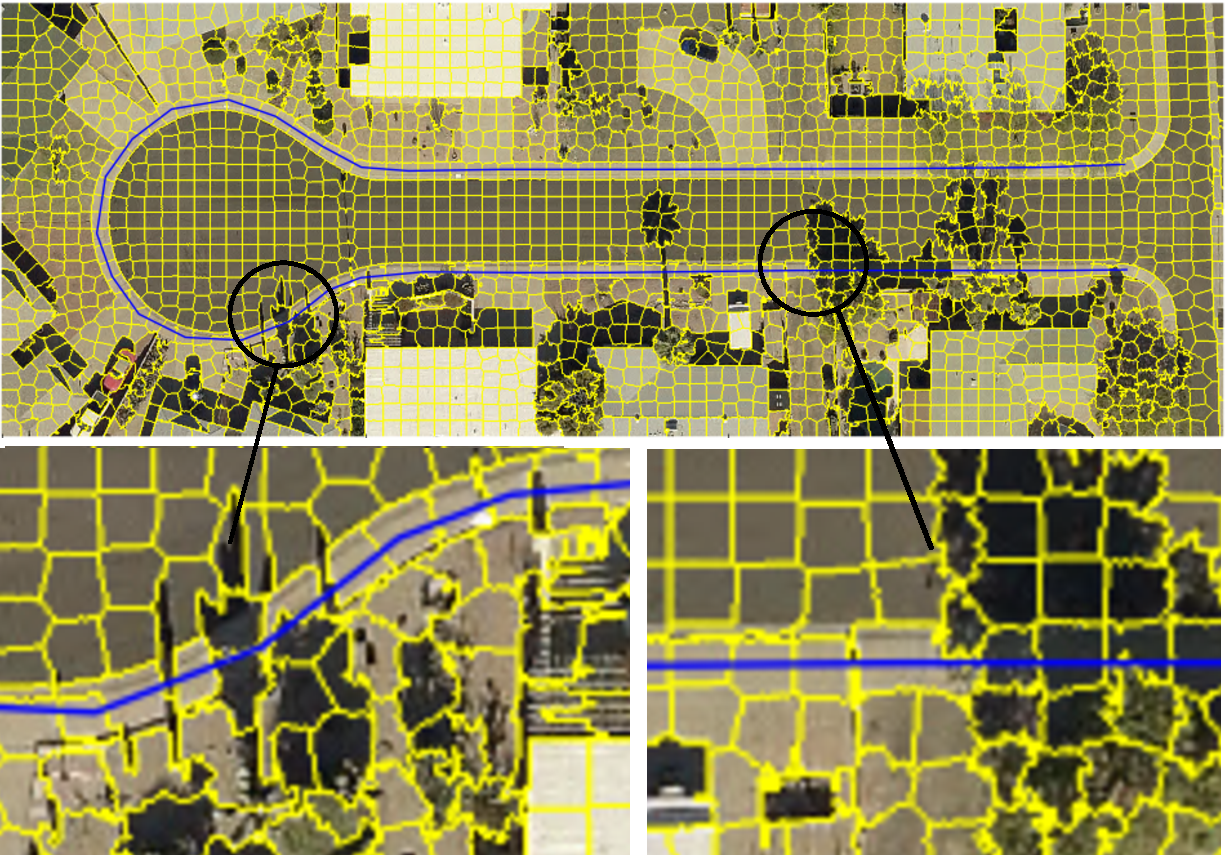
\includegraphics[width=\textwidth]{Figures/slic_sample1.pdf}
    \caption[Example of Simple Linear Iterative Clustering]{Detail demonstration on segmenting large image into irregularly shaped super-pixels with \ac{SLIC}. Row 2 indicates examples of false positive, with recognized a non-sidewalk feature (shadow) as a part of sidewalk.}
    \label{fig:slic}
\end{figure}

Simple linear iterative clustering (SLIC) works with super-pixels, which segment a large image into different irregularly shaped regions of homogeneous appearance or texture \cite{Achanta:149300}. It uses the compact evenly distributed homogeneous regions of an image as a pre-processing step, so that image segmentation can be accomplished by grouping super-pixels which snap to natural boundaries in an image. Alternatively, super-pixels can initiate a region growing process\cite{Borovec2017-fz}. As shown in figure \ref{fig:slic}, slic will identify a non-sidewalk feature as positive if there is a shadow covering the sidewalk, which may lead to over mark the boundary (\aclp{FP}). This becomes a problem since all super-pixels that we decide to use are based on a line in between both edges of sidewalk which we marked as ground truth. On the one hand, if the super-pixel above lay on the line, we got an error, since we marked part of the feature that not the sidewalk on the sidewalk, which gives us \aclp{FP}. On the other hand, if that super-pixel does not lay on the line, we missed a part that's clear is the sidewalk. Thus, finding a way to separate such a feature become important. Trying to decrease the size of the width of each super-pixel was one of the ways to fix it but may cause an incompleteness since each super-pixel is smaller than the width of the sidewalk. So the idea of width control become important.

\section{Active Contours}

\begin{figure}[H]
    \centering
    \includegraphics[width=\textwidth]{Figures/ac1.png}
    \caption[Example of Active Contours]{Detail demonstration with active contours method. Row 2 indicates examples of false positive, which is recognized a non-sidewalk feature (shadow) and similar texture (driveway) as a part of sidewalk.}
    \label{fig:ac}
\end{figure}

A very successful region growing process is snakes, or Active Contours, which starts with an approximate contour and evolves the boundary to optimize an energy function that favors likely contour shapes. Compared with the other two segmentation tools, active contour may not be the best solution for identifying ribbon-like feature since it is not the best tool to separate blurred edges. Al-Diri \cite{ActiveContou09} proposed using active contour to identify each edge separately, in the mean time keep maintaining width consistency. It is a good approach but it is not ideal to apply on our problem, since their ribbon-like feature (vessels) does not requiring predict edges under obstacles, such as trees or cars that above the sidewalk.


Both \ac{SLIC} and active contours start from an initial shape to find precise boundaries by solving a \ac{CRF} problem. In addition, graph cuts are capable of global \ac{CRF} problem. In addition, graph cut are capable of global \ac{CRF} optimization in some situations, and iterative graph cut are used by the GrabCut algorithm to refine an initial segmentation \cite{Rother2004-ou}. However in figure \ref{fig:Method_comparison} and figure \ref{fig:ac}, we show the segmentation results of these methods, and note that they struggle to constrain their results to ribbon-like shapes with smooth thickness and mid-line. These color or boundary smoothness methods fail to capture an important quality of ribbon-like features, which is the thickness at one point depends not only its adjacent points but also its topologically distant points along the contour.

\section{\ac{CNNs}}

Another image segmentation approach that has seen extraordinary success is the use of \ac{CNNs} and transposed convolution \cite{Badrinarayanan2017-il, Noh2015-ni, Shelhamer2017-rf, Ronneberger2015-sv}. Unlike the proposed approach, these have millions of tunable parameters and need significant pre-annotated data and offline training to build a model. In a recent exploration of learning to segment street networks from online maps \cite{Kaiser2017-np}, built a fully convolutional network with 137 million parameters. A similar approach with another deep architecture called U-net\cite{Ronneberger2015-sv} was applied to the street network segmentation problem \cite{Zhang2017-gi}. These approaches claim to be robust to occlusion and ambiguous regions, but they benefit from a large amount of carefully annotated data that includes road width \cite{Mnih2013-dp}. This type of pre-annotated data with aligned aerial imagery is much harder to obtain for walking paths. The proposed approach has only handful of tunable parameters with clear interpretations, so that they can be interactively set and used without offline training.

% \section{boss paper}
\chapter{A Dynamic Programming Approach}

We import LiDAR data and shape-file that contain geometric information of the location for each sidewalk. 
Instead of analysis the texture difference between desire sidewalk and non-sidewalk feature, we treat it as the ribbon-like feature and try to segment them base on their growth from start point. 

% \begin{figure}[H]
%     \centering
%     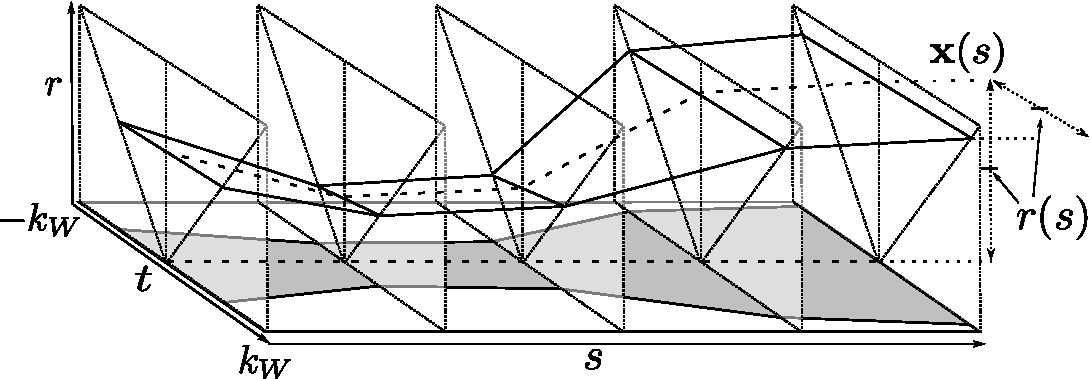
\includegraphics[width=\textwidth]{Figures/ribbon-3d.pdf}
%     \caption[3D Ribbon Image]{An illustration of the parameters for a ribbon; the $r$ axis captures the thickness of the ribbon and the $s$ axis captures the distance along the initial ribbon. The $t$ axis records horizontal displacements from the initial ribbon's medial curve.}
%     \label{fig:ribbon_3d}
% \end{figure}

\begin{figure}[htb]
    \centering
    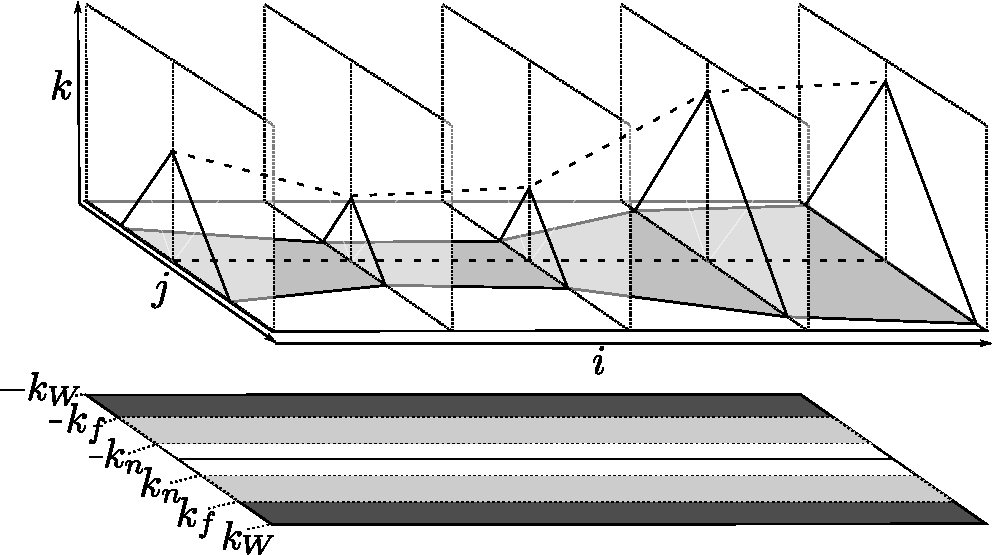
\includegraphics[width=\textwidth]{Figures/ribbon-3d-combined.pdf}
    \caption[3D Ribbon Image]{An illustration of the parameters for a ribbon: (top) the $k$ axis captures the thickness of the ribbon and the $i$ axis captures the distance along the initial ribbon, the $j$ axis records horizontal displacements from the initial ribbon's medial curve; (bottom) the boundaries of the ribbon must lie within $\pm \MaxDistance{}$, pixels within $\pm \MinRadius{}$ of the center are probably part of the ribbon and pixels further than $\pm \MaxRadius{}$ are likely negative. }
    \label{fig:ribbon_3d}
\end{figure}

\section{The Ribbon Image}

In order to simplify the problem, we first create a straightened "ribbon" image in which the sidewalk runs in a straight line, even if the original sidewalk if curved.
We represent a ribbon of length $L$ using parameters along and orthogonal to a medial curve $\mathbf{x}(s)$, where $s \in [0, L]$. The ribbon image is the set of all points within a perpendicular distance $r(s)$ to the medial curve.

A second parameter, which we call $t$, is measured in a direction orthogonal to the curve.  
We define ribbon coordinates $\mathbf{x}(s, t) = \mathbf{x}(s) + t\mathbf{n}(s)$, where $\mathbf{n}(s)$ is a vector perpendicular to the medial curve at position $s$, which can be obtained by rotating the curve's tangent vector $\dot{\mathbf{x}}(s)$ by 90 degrees. 


In practice we represent the curve $\mathbf{x}(s)$ discretely as an arc-length re-sampled set of points $\mathbf{x}_s,$ for $s=0,1,...,L-1$ from poly-line features that are read from a GIS file. The points are sampled at an arc-length distance of about one pixel between each point, and then Laplacian smoothing is applied in order diffuse the curvatures along the re-sampled poly-line.  
We use a secant to estimate the tangent to the curve,
\[\dot{\mathbf{x}}_s = \left[\begin{array}{c} \dot{x}_s \\ \dot{y}_s \end{array}\right]= \frac{\mathbf{x}_{s+1}-\mathbf{x}_{s-1}}{||\mathbf{x}_{s+1}-\mathbf{x}_{s-1}||} \] and rotate it ninety degrees counter-clockwise in order to find a direction  $\mathbf{n}_s$, so that 
\[\mathbf{n}_s = \left[\begin{array}{c} -\dot{y}_s \\ \dot{x}_s \end{array}\right]. \]

\begin{figure}[H]
    \centering
    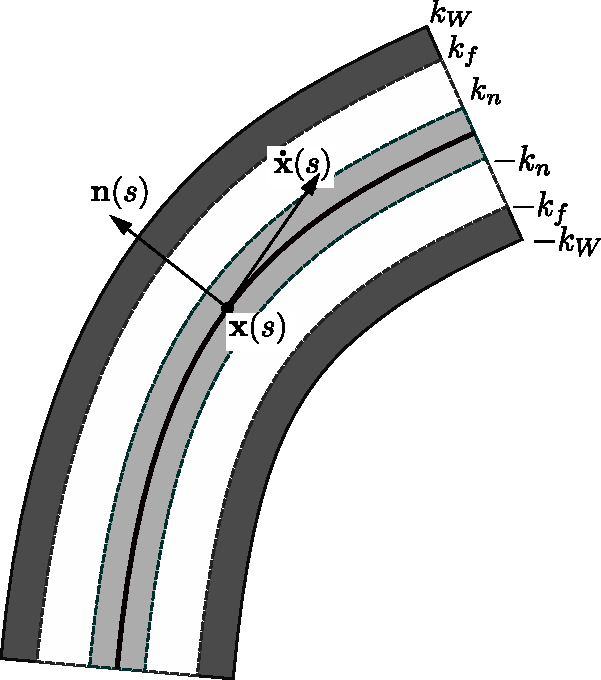
\includegraphics[width=\textwidth]{Figures/sw-figure.pdf}
    \caption[2D Ribbon Image]{A demonstration of the parameters for a ribbon in 2D. $k_n$ indicates a parameter that describes the radius of the medial curve that we considered to be part of the ribbon, $k_f$ is a distance from the medial curve that we considered very unlikely to be part of the ribbon, and $k_W$ is the maximum width of the ribbon image.}
    \label{fig:2d_ribbon}
\end{figure}

As shown in \ref{fig:2d_ribbon}, from figure \ref{fig:osm_oxford_path}, we should assume that there is some uncertainty in the position $\mathbf{x}_s$ of the medial curve and also uncertainty in the radius $r_s$ of the discredited ribbon. 
But that there is range of distances $t \in 0\dots k_n$ from the medial curve which we can accept labeling as positive examples that are within the ribbon, and that there is some range of distances $t \in k_f\dots k_W$ which we can accept labeling as negative sample. 
Finally a range $t\in (k_n+1)...(k_f-1)$ of distances that are possible locations of the ribbon's boundary.
Therefore, when searching for improved medial curves and radii of the ribbon, we can consider a discrete range of offsets $t=-k_W,..., k_W$ chosen to be wide enough that true ribbon image itself likely fits entirely within the grid of input negative samples along its edges.  

The orthorectified color image $\image(x,y)$
records the color at the point $x,y$ in the image plane.
Then $\image(\mathbf{x}_{s,t}),$ is a warped version of the image in which the ribbon is centered on a single strip at $t=0$.
The situation is illustrated in \ref{fig:ribbon_3d}.  
In this warped image, we can estimate the amount $t_s$ to shift the ribbon's center in the $t-$axis, which is orthogonal to the curve,  and also the amount the radius $r_s$ so that the  ribbon at each row is in columns $(t_s - r_s)\dots(t_s+r_s)$.  
Our problem is to estimate the most likely values of $t_s$ and $r_s$.  


\section{Initial Density Estimation}

\begin{figure}[H]
    \centering
    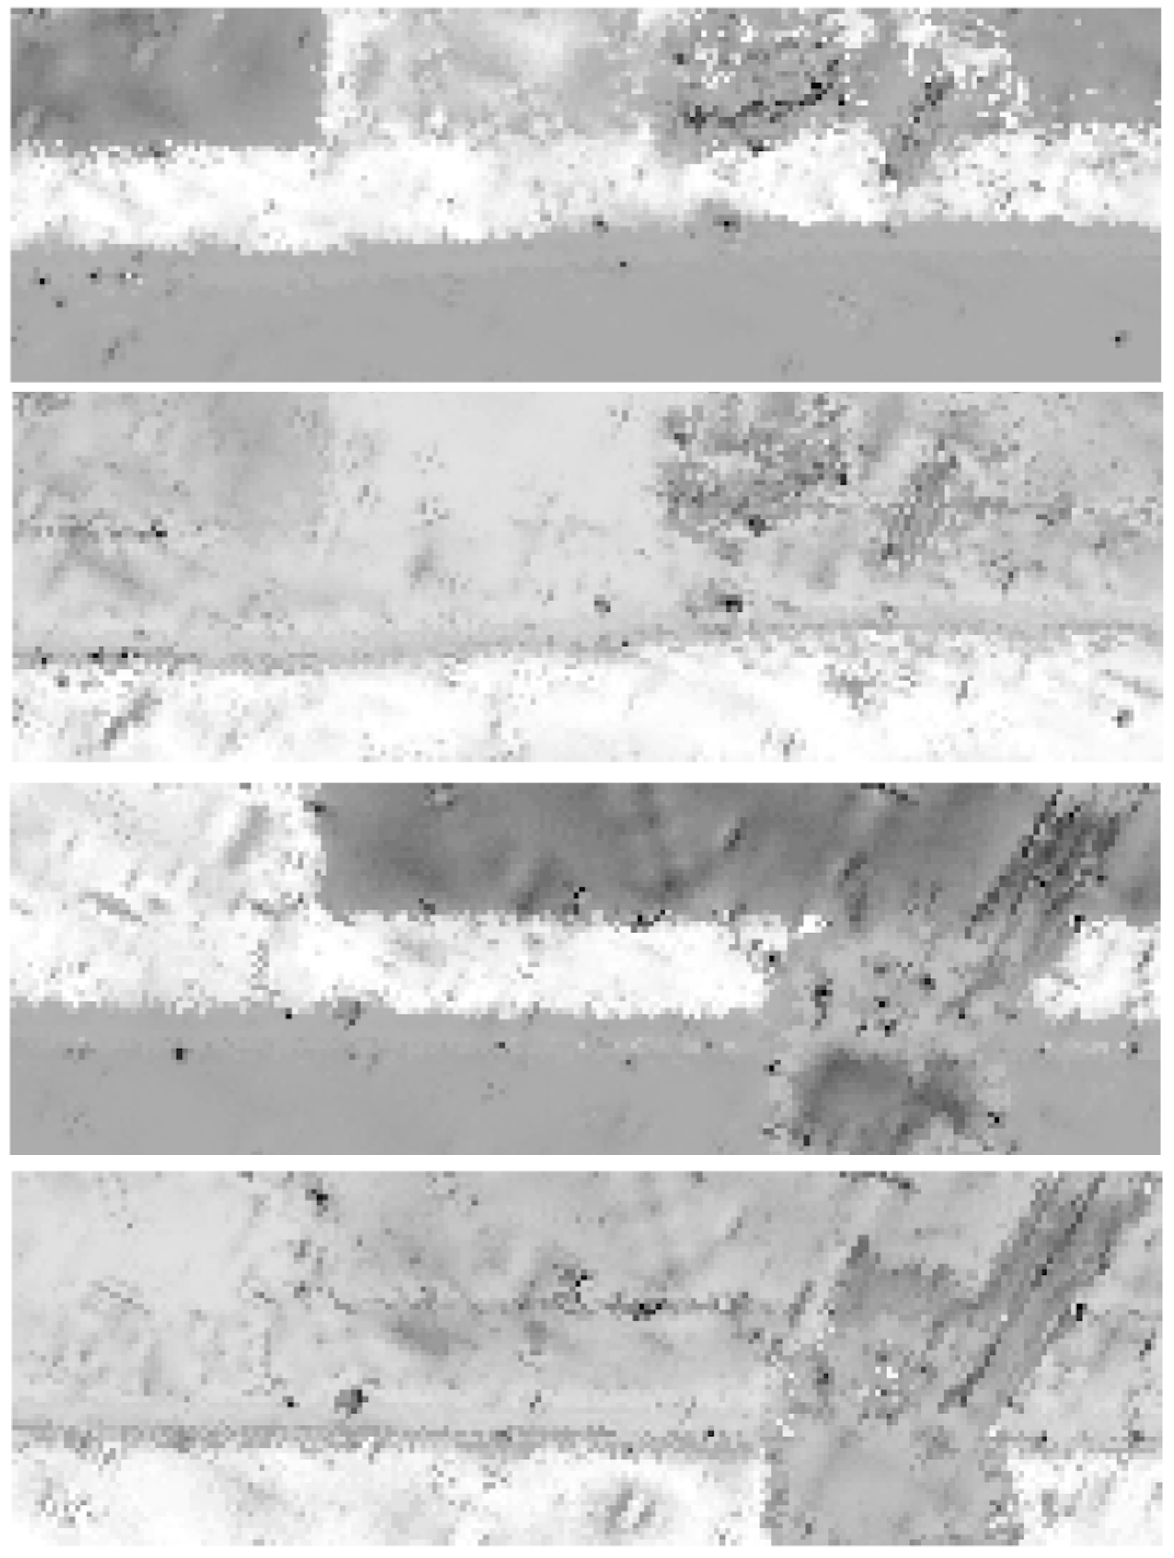
\includegraphics[width=0.8\textwidth]{Figures/gmm_sample_1.png}
    \caption[\ac{GMM} Result 1]{Example of GMMs on sample sidewalk. The first row and third row shows the foreground GMM for sample sidewalk, and the second row and fourth row shows the back-ground for simple sidewalk. We use grey-scale to show the changes of probabilities, where for foreground, white is more likely to be sidewalk, and black is not.}
    \label{fig:GMM_result}
\end{figure}


We aim to find a segmentation that combines \textit{shape} priors on the curvature and thickness of the ribbon-like features and also maximizes the likelihood of observing colors in the image. 
Let $\Lambda$ be a random variable for the event that a color $\lambda$ is observed in an image, and let $R$ indicate a random variable so that $R=1$ if a pixel is part of ribbon and $R=0$ if a pixel is not. 
A variety of approaches exist to learn the conditional probability $\Pr(\Lambda|R)$ of observing a color conditioned on whether a pixel within or outside of a ribbon \cite{hartigan1979algorithm, jordan1999introduction}.
Many of these methods take as input a set of training examples in order to choose parameters for some model.
Our conjecture is that the initial estimate of our sidewalk's mid-line, while perhaps not perfect, is much more likely to cover pixels that are part of a sidewalk than the pixels at the edge of the ribbon image. 

We use this assumption to estimate the probability that a pixel is part of a ribbon conditioned on its color.
Let $k_n$ be parameter that describes the radius around the medial curve that we will consider to be part of the ribbon with very high confidence. 
Let $k_f$ indicate a distance from the medial curve that we consider very unlikely to be part of the ribbon. 
Finally, let $k_W$ indicate maximum value of $t$ to consider when learning the distribution of colors in a ribbon image. 
We model the distribution of colors within the sidewalk as a Gaussian Mixture Model of $k_g=4$ full-co-variance gaussian distribution and we model the distribution of colors outside of the ribbon as a mixture $2k_g$ Gaussian since we expect more variation and complexity in this zone. 
As shown in figure \ref{fig:GMM_result}, given an initial estimate for the set of colors inside or outside of the ribbon, we estimate the weights and co-variances of the Gaussians using the \ac{EM-GMM} \cite{sridharan2014gaussian} algorithm. 


\section{A Lattice Representation of the Problem} 
We represent the solution to this problem as graph where each node represents a point that may lie on the middle of a ribbon with a different width, and edges connect each node to a node that may have preceded it on a path. 

We will assume that widths may take on values from a set of predefined odd numbers (so that there is always a pixel in the center) 
Then the negative log-likelihood of for a particular pair of values $t_s$ and $r_s$ at a single row $(s)$ is 

\begin{align}
\rownll(s, t_s, r_s) &= -\log \Pr(r_s, t_s)  + \sum_{t} \pixelnll(s,t, t_s, r_s) \\
\pixelnll(s, t, t_s, r_s) &= 
\begin{cases}
 -\ln\Pr(\image(\x_{s,t})|\x_{s,t} \in R) &\text{if } t\in [t_s-r_s, t_s+r_s]\\
 -\ln\Pr(\image(\x_{s,t})|\x_{s,t}\not\in R) &\text{if } t\not\in[t_s-r_s, t_s+r_s]
\end{cases}
\end{align}

which combines the probabilities of seeing each color at offset $s$ in the ribbon image conditioned on whether the color is inside or outside of the ribbon.
However, we assume ribbons are continuous with respect to the position of their mid-line and their thickness, likelihood of the most probable path up to offset $s$ is 

\begin{align}
\ribbonnll(s, t_s, r_s) &=  \begin{cases}
-\log \Pr(r_s, t_s) & \text{if } s = 0\\
   \begin{aligned}
   & \rownll(s, t_s, r_s) \\ 
   & + \displaystyle\max_{\delta_t,\delta_r} [p(\delta_t, \delta_r)+\ribbonnll(s-1, t_s+\delta_t, r_s+\delta_r)]
   \end{aligned} & \text{if } s > 0.\\
\end{cases}
\end{align}

The quantity $p(\delta_t, \delta_r)$ is a penalty for changing direction or thickness, and could be set to the negative log likelihood of observing a change $\delta_t$ in position and a change $\delta_r$ in thickness. 
For discrete choices of $\delta_t$ and $\delta_r$ these costs can be represented by number in a matrix.

% \begin{algorithm}
% \caption{A Dynamic programming approach predict edges for ribbon-like feature}

% \begin{algorithmic}
% \State Initialize a matrix $A$ to same shape as ribbon image
% \For {each line of pixel $s$ in ribbon image}
%     \For{each possible pixel as $t_s$ in width of line}
%         \For{each pixel as $r_s$ in between $t_s$ and edge of line}
%             \State Store the returned probabilities from function D in $A[0, ts, rs]$
%             \If{not the first line pixel}
%                 \For {each $\delta_t and \delta_r \in \{-1, 0, 1\}$}
%                     \State Store max sum value from returned probability,
%                     \State $A[s-1, t_s+\delta_t, r_s+\delta_r]$ and penalty in $A[s, t_s, r_s]$
%                     \State Also store the value of $\delta_t$ and $\delta_r$
%                 \EndFor
%             \EndIf
%         \EndFor
%     \EndFor
% \EndFor


% \end{algorithmic}
% \end{algorithm}
\chapter{Publication}

The main steps of our approach are illustrated in \figref{fig:Apparatus}; a \ac{VHR} orthorectified image is provided and a the approximate trajectory of a sidewalk is acquired from a \ac{GIS} such as \ac{OSM}. Alternately, an approximate trajectory could be marked by a person to digitize the sidewalk quickly. The initial trajectory is re-sampled and used to warp a portion of aerial image so that the trajectory is mapped to a straight, horizontal line which we call a \textit{ribbon image}.  We use a modest assumption that colors near the center of the ribbon image are more likely to be on a walking path in order to build a probability-density estimate for walking path materials. Based on the probability estimate at each pixel, we construct a single ribbon with priors that control the rate of change of thickness and direction of the ribbon. Finally, the boundaries are warped back onto the original reference frame. In this section we elaborate the process of generating a ribbon image, estimating the probability that a color belongs to the same material as a walking path, and the construction of a smooth ribbon image based on the resulting probabilities. 

\begin{figure}[H]
\begin{center}
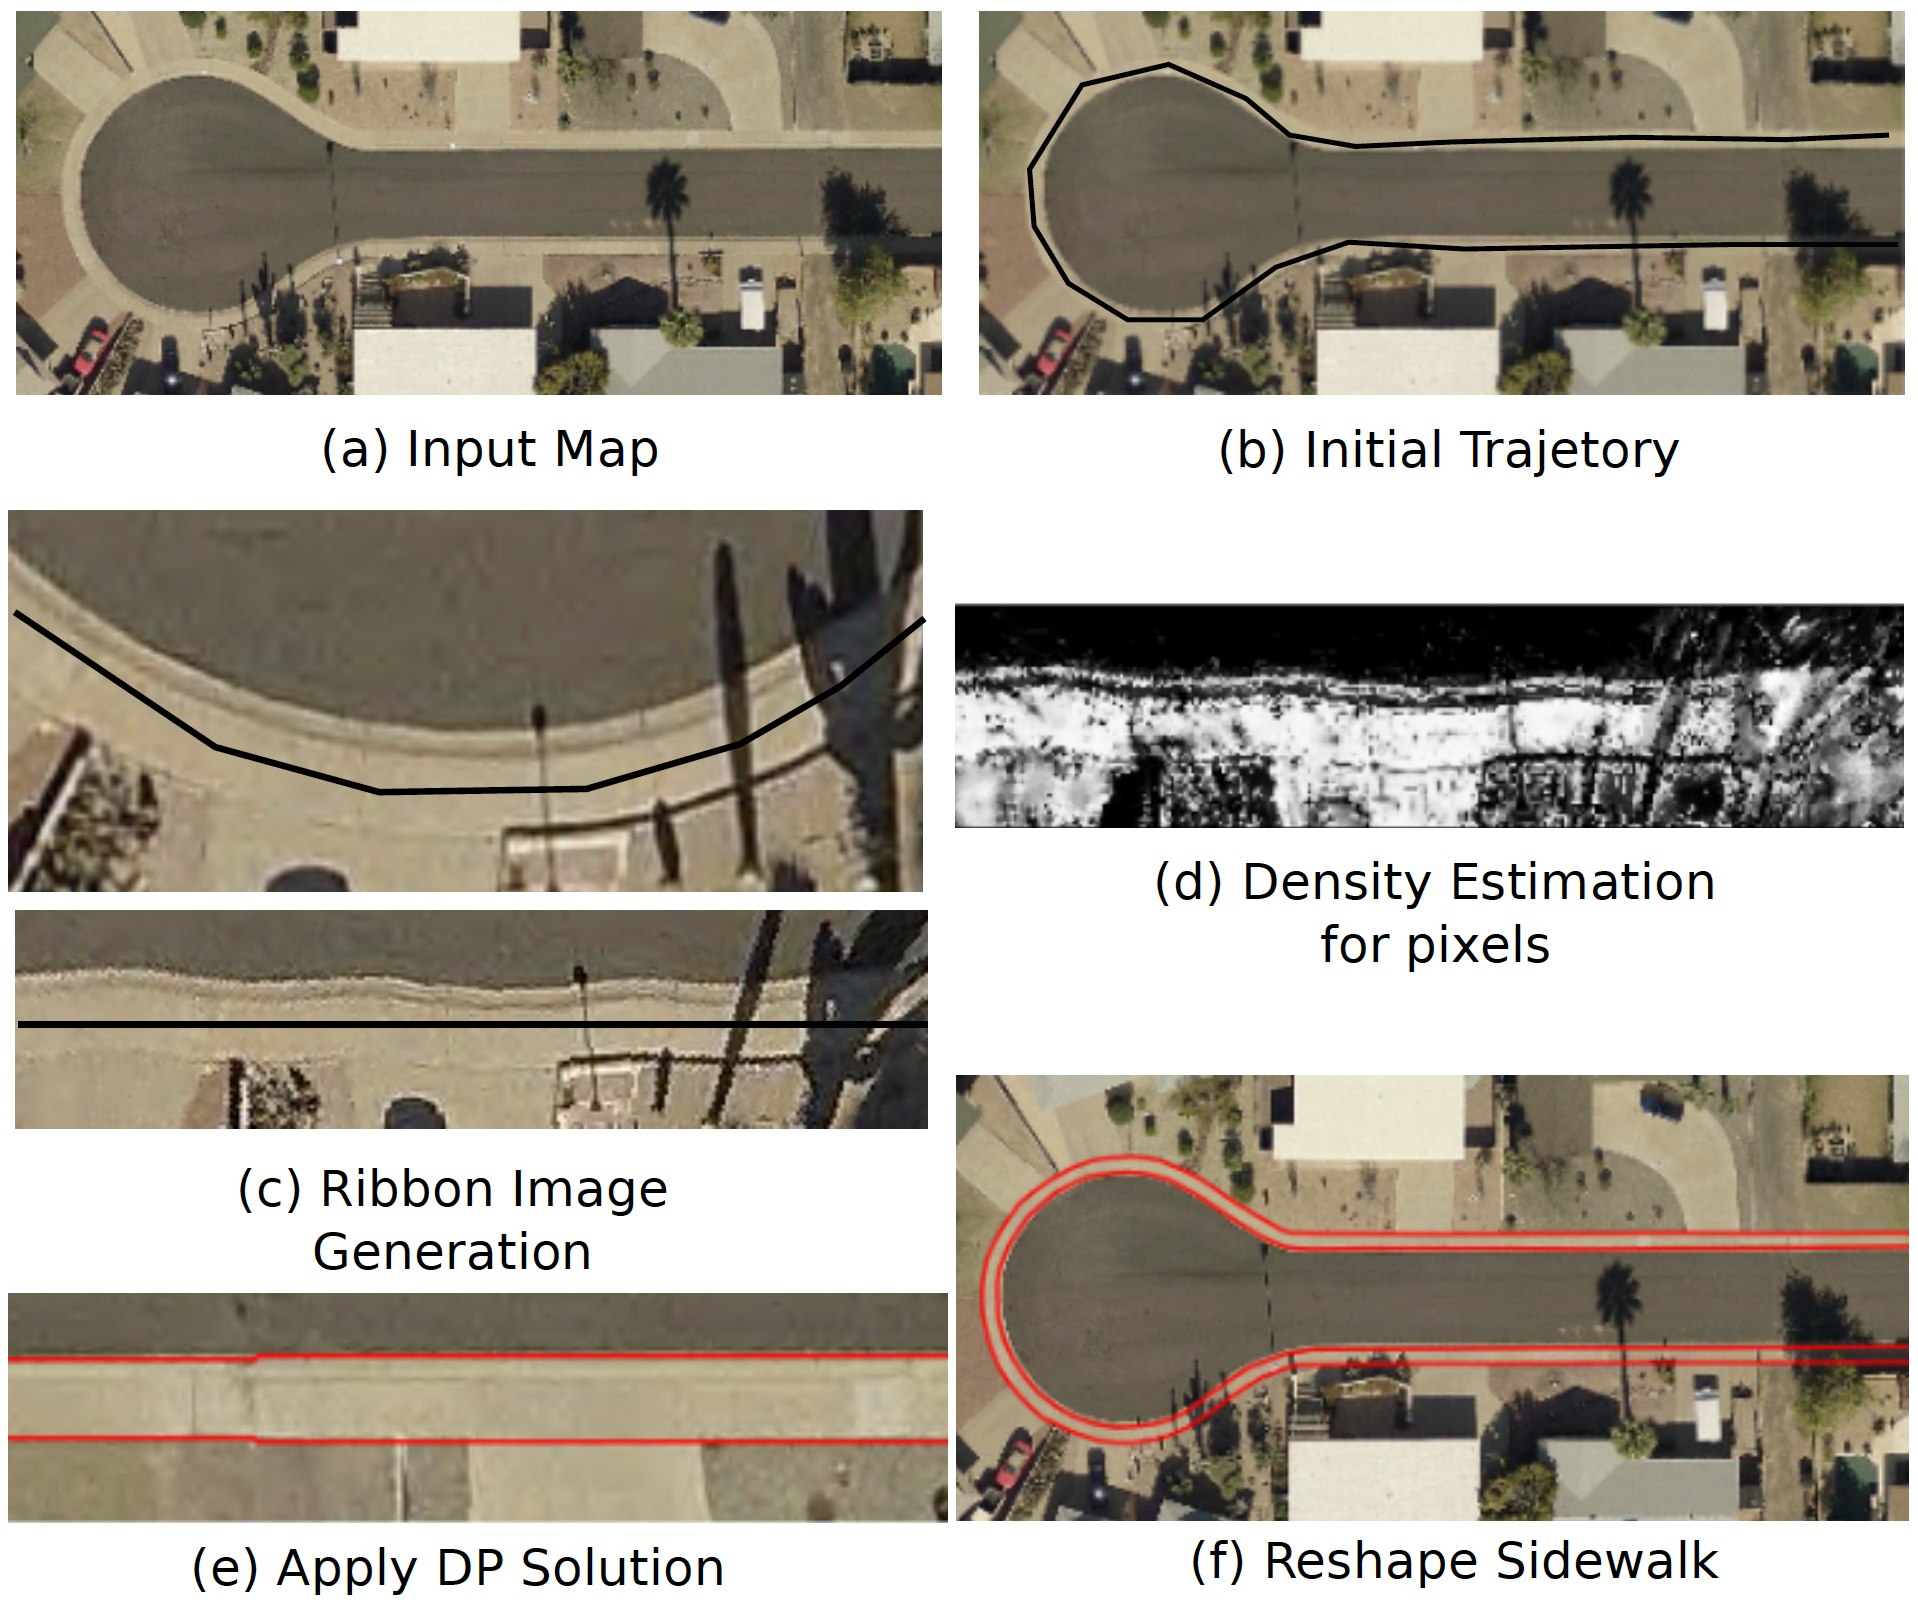
\includegraphics[width=0.9\textwidth]{Figures/diagram.png}
\caption[Framework Overview 2]{Our approach adopted to predict precise boundaries for ribbon-like features. Where black line indicated a sidewalk's geometric information, and red lines shown our result for the sidewalk boundaries. From (a) to (f), the 6 step approach introduce input map (a), initial trajectory (b), ribbon image generation (c), density Estimation for pixels(d), apply \ac{DP} solution(e), reshape sidewalk(f).}
\label{fig:Apparatus}
\end{center}
\end{figure}

\section{Warping an input image}

We take as input an image $\InputImage{}$ and a trajectory $\InputTrajectory{}=\langle \vec{p}_0, \vec{p}_1,\dots,\vec{p}_m\rangle$ where each $\vec{p}_i=(x_i, y_i)^T$ is a point on the initial estimate of a ribbons trajectory (re-sampled and smoothed). Further, we are able to estimate unit-length tangent vectors $\vec{u}_i$ and their perpendiculars $\vec{v}_i$; for example by using the secant method 
\begin{align}
  \vec{u}_i &= \frac{\vec{p}_{i+1}-\vec{p}_{i-1}}{\|\vec{p}_{i+1}-\vec{p}_{i-1}\|} \\
  \vec{v}_i &= \left(\begin{array}{cc}
       0  & 1 \\
       -1 & 0
  \end{array} \right) \vec{u}_i
\end{align}
where the endpoints are repeated. We define the warped ribbon-image $\RibbonImage{}$ so that $\RibbonImage{[i,j]}=\InputImage{}(\vec{p}_i+ j \vec{v}_i)$. We use the convention that square-brackets to indicate discrete indices and rounded parenthesis indicate interpolated samples.  An example of the process is shown in \figref{fig:Sample_Sidewalk_4} and \figref{fig:Apparatus}(c). 

\begin{figure}
    \centering
    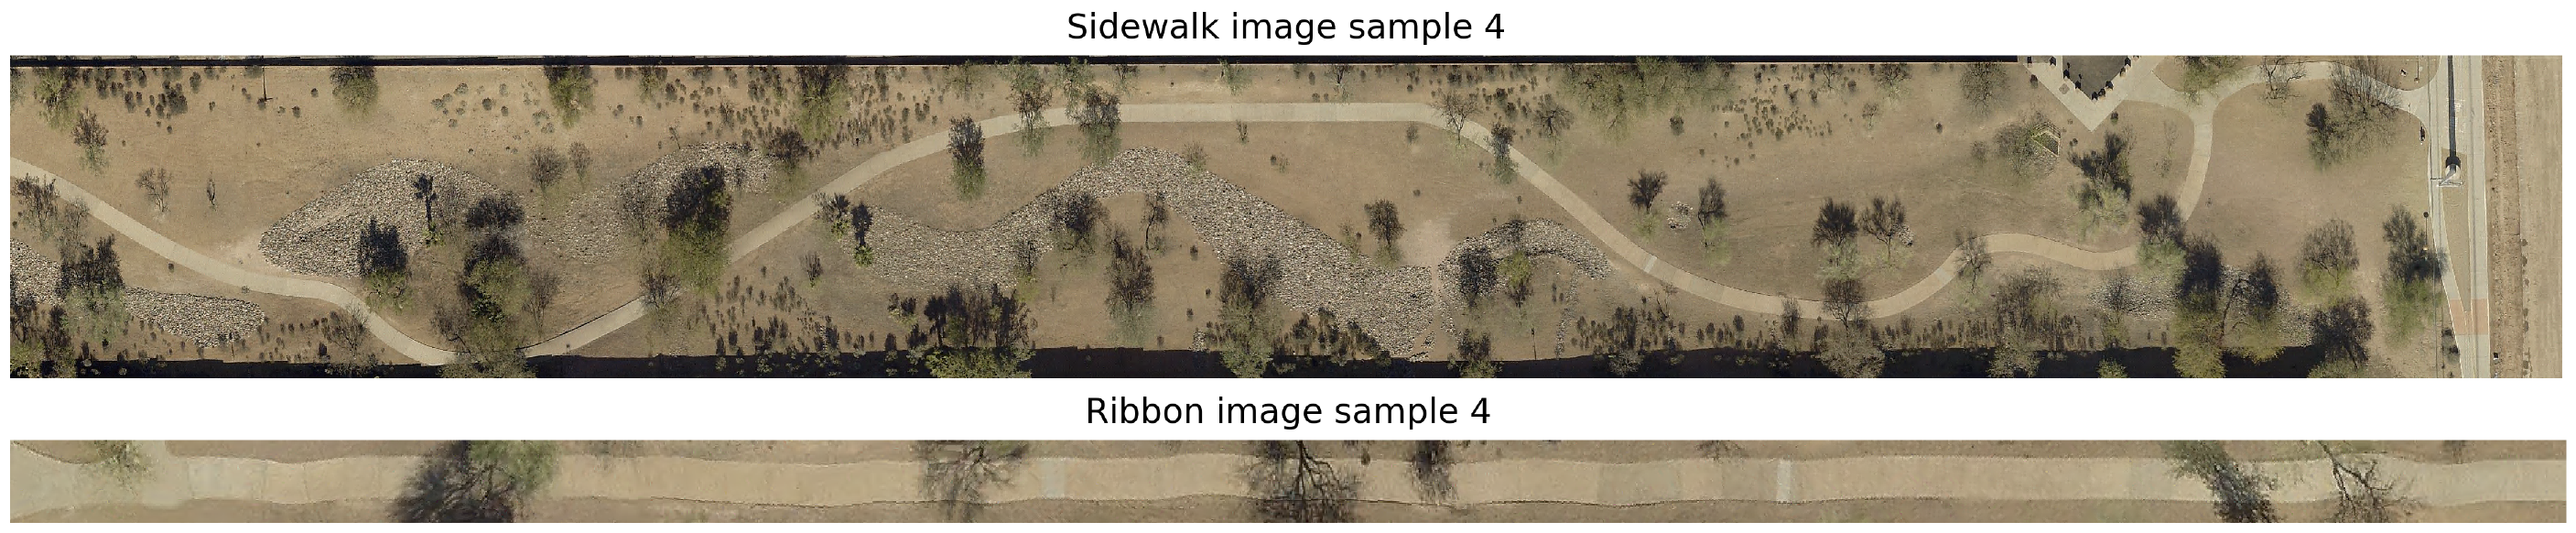
\includegraphics[width=\textwidth]{Figures/Sample4_needed.png}
    \caption[Sample Sidewalk 1]{A ribbon image straighten output which used the previous process from figure \ref{fig:StraightenProcess} to convert an original image into ribbon image .}
    \label{fig:Sample_Sidewalk_4}
\end{figure}

% \begin{figure}[ht]
%     \centering
%     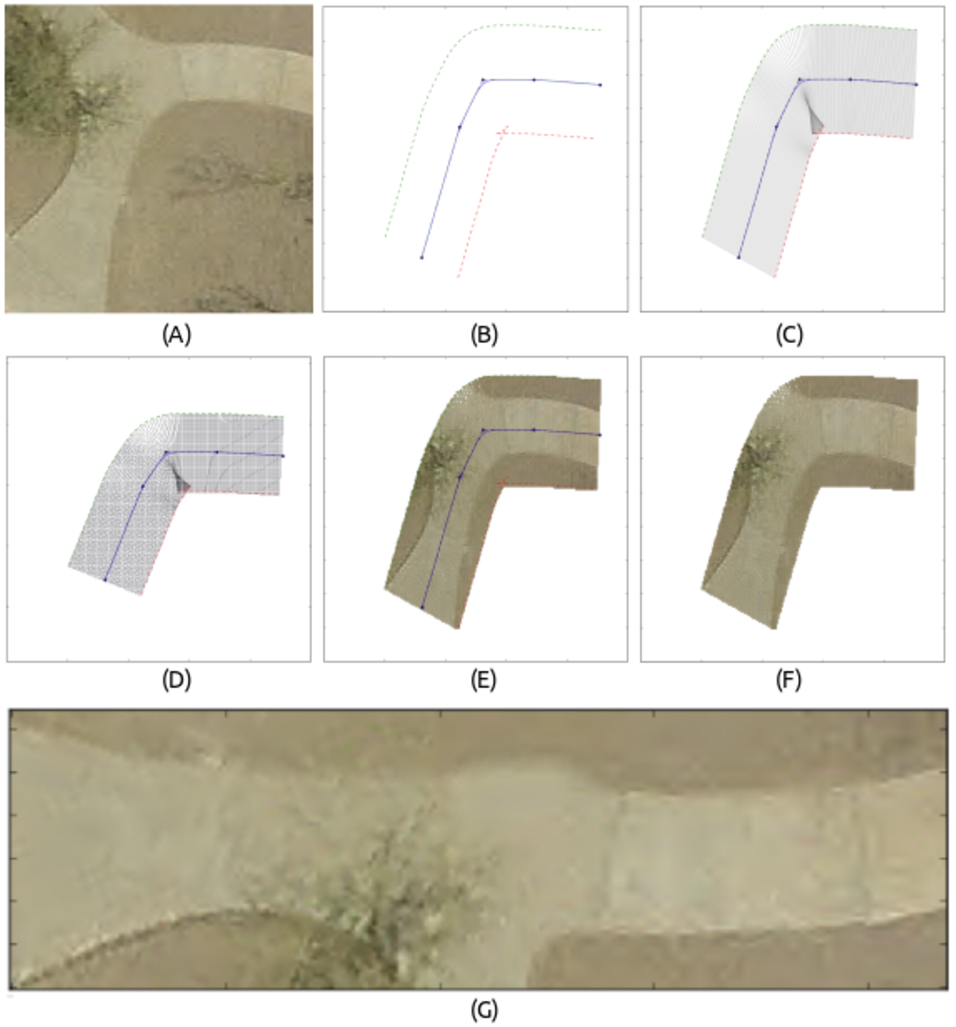
\includegraphics[width=0.95\columnwidth]{Figures/straghten.pdf}
%     \caption[Ribbon Image Generation]{Ribbon image generating process: (a) raw input $\InputImage{}$, (b) we densely resample and smooth the trajectory using $\MaxRadius{}$ iterations of Laplacian smoothing and show the locations of warped pixels of $\RibbonImage{}$ within $\pm \MaxDistance{}$;  (c) the warped ribbon image $\RibbonImage{}$ shown in the original reference frame and  (d) the generated the ribbon image (shown transposed to fit in the figure).}
%     \label{fig:StraightenProcess}
% \end{figure}

% \begin{figure}[ht]
%     \centering
%     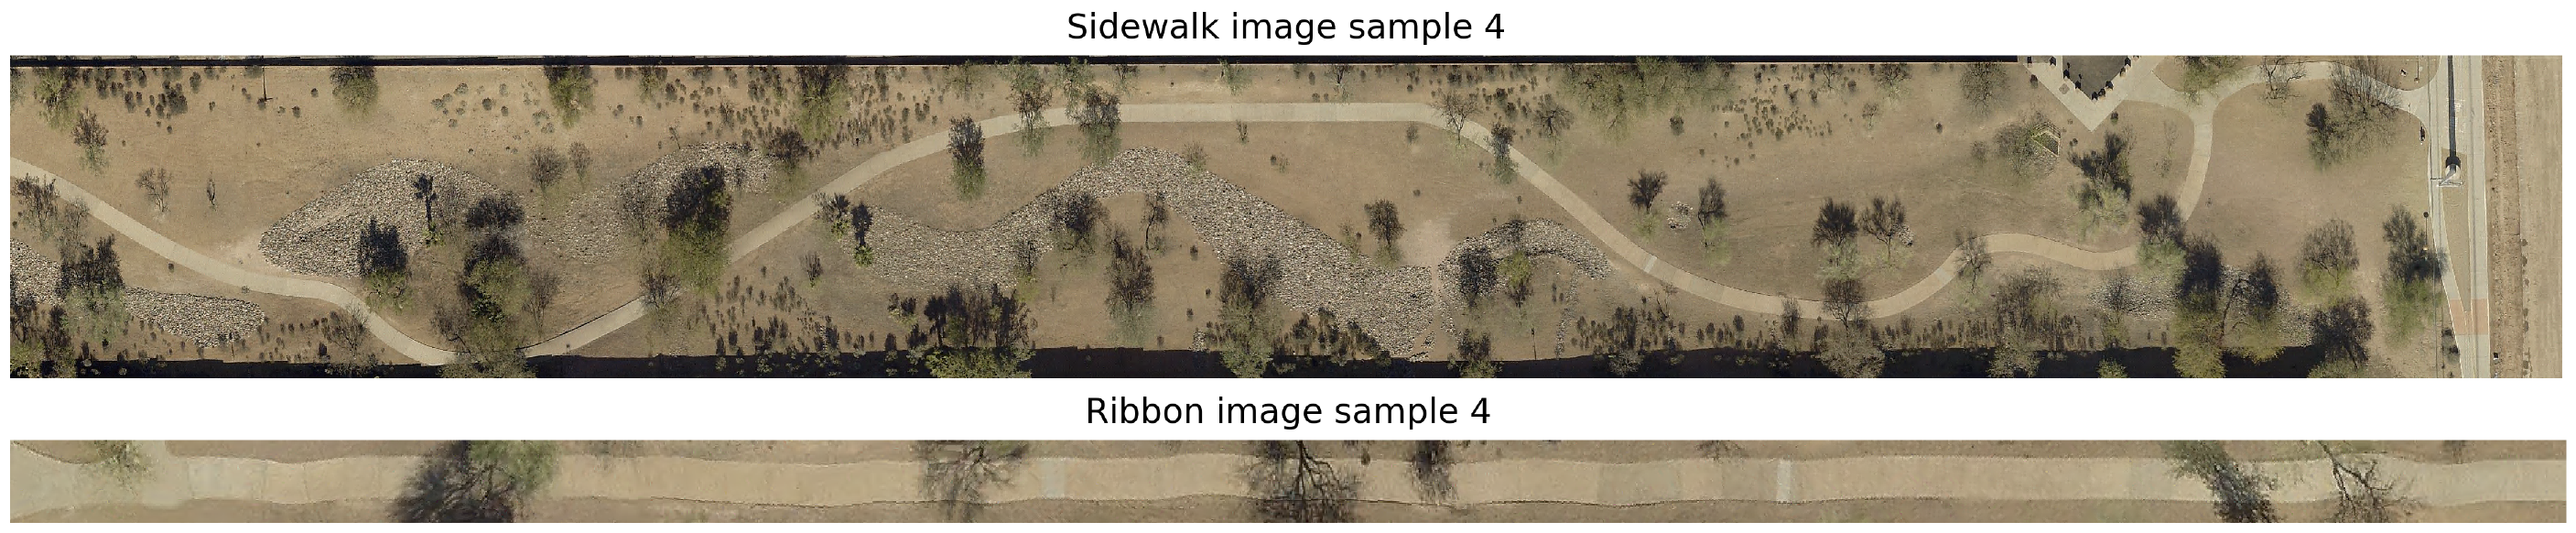
\includegraphics[width=0.95\columnwidth]{Figures/Sample4_needed.png}
%     \caption[Sample Sidewalk]{A ribbon image; the original image $\InputImage{}$ (top) was warped so that the trajectory is a straight line to create a ribbon image $\RibbonImage{}$ (bottom), shown transposed.}
%     \label{fig:Sample_Sidewalk_4}
% \end{figure}

\section{Density Estimation}
We aim to find a new trajectory $\OutputTrajectory{[0\dots m]}$ and radius $\OutputRadius{[0\dots m]}$ that are most likely given an input image. We first must estimate the probability of observing a color within the ribbon.  
Given an input image $\RibbonImage{}$, let $\Pr(\text{pos}|\phi,\theta)$ denote the probability that a pixel is a part of a ribbon given an observed color $\phi$ and set of learnable parameters $\theta$. 
We aim to estimate parameters $\theta$ that maximize the likelihood of our \textit{initial} path. 

\begin{figure}[H]
    \centering
    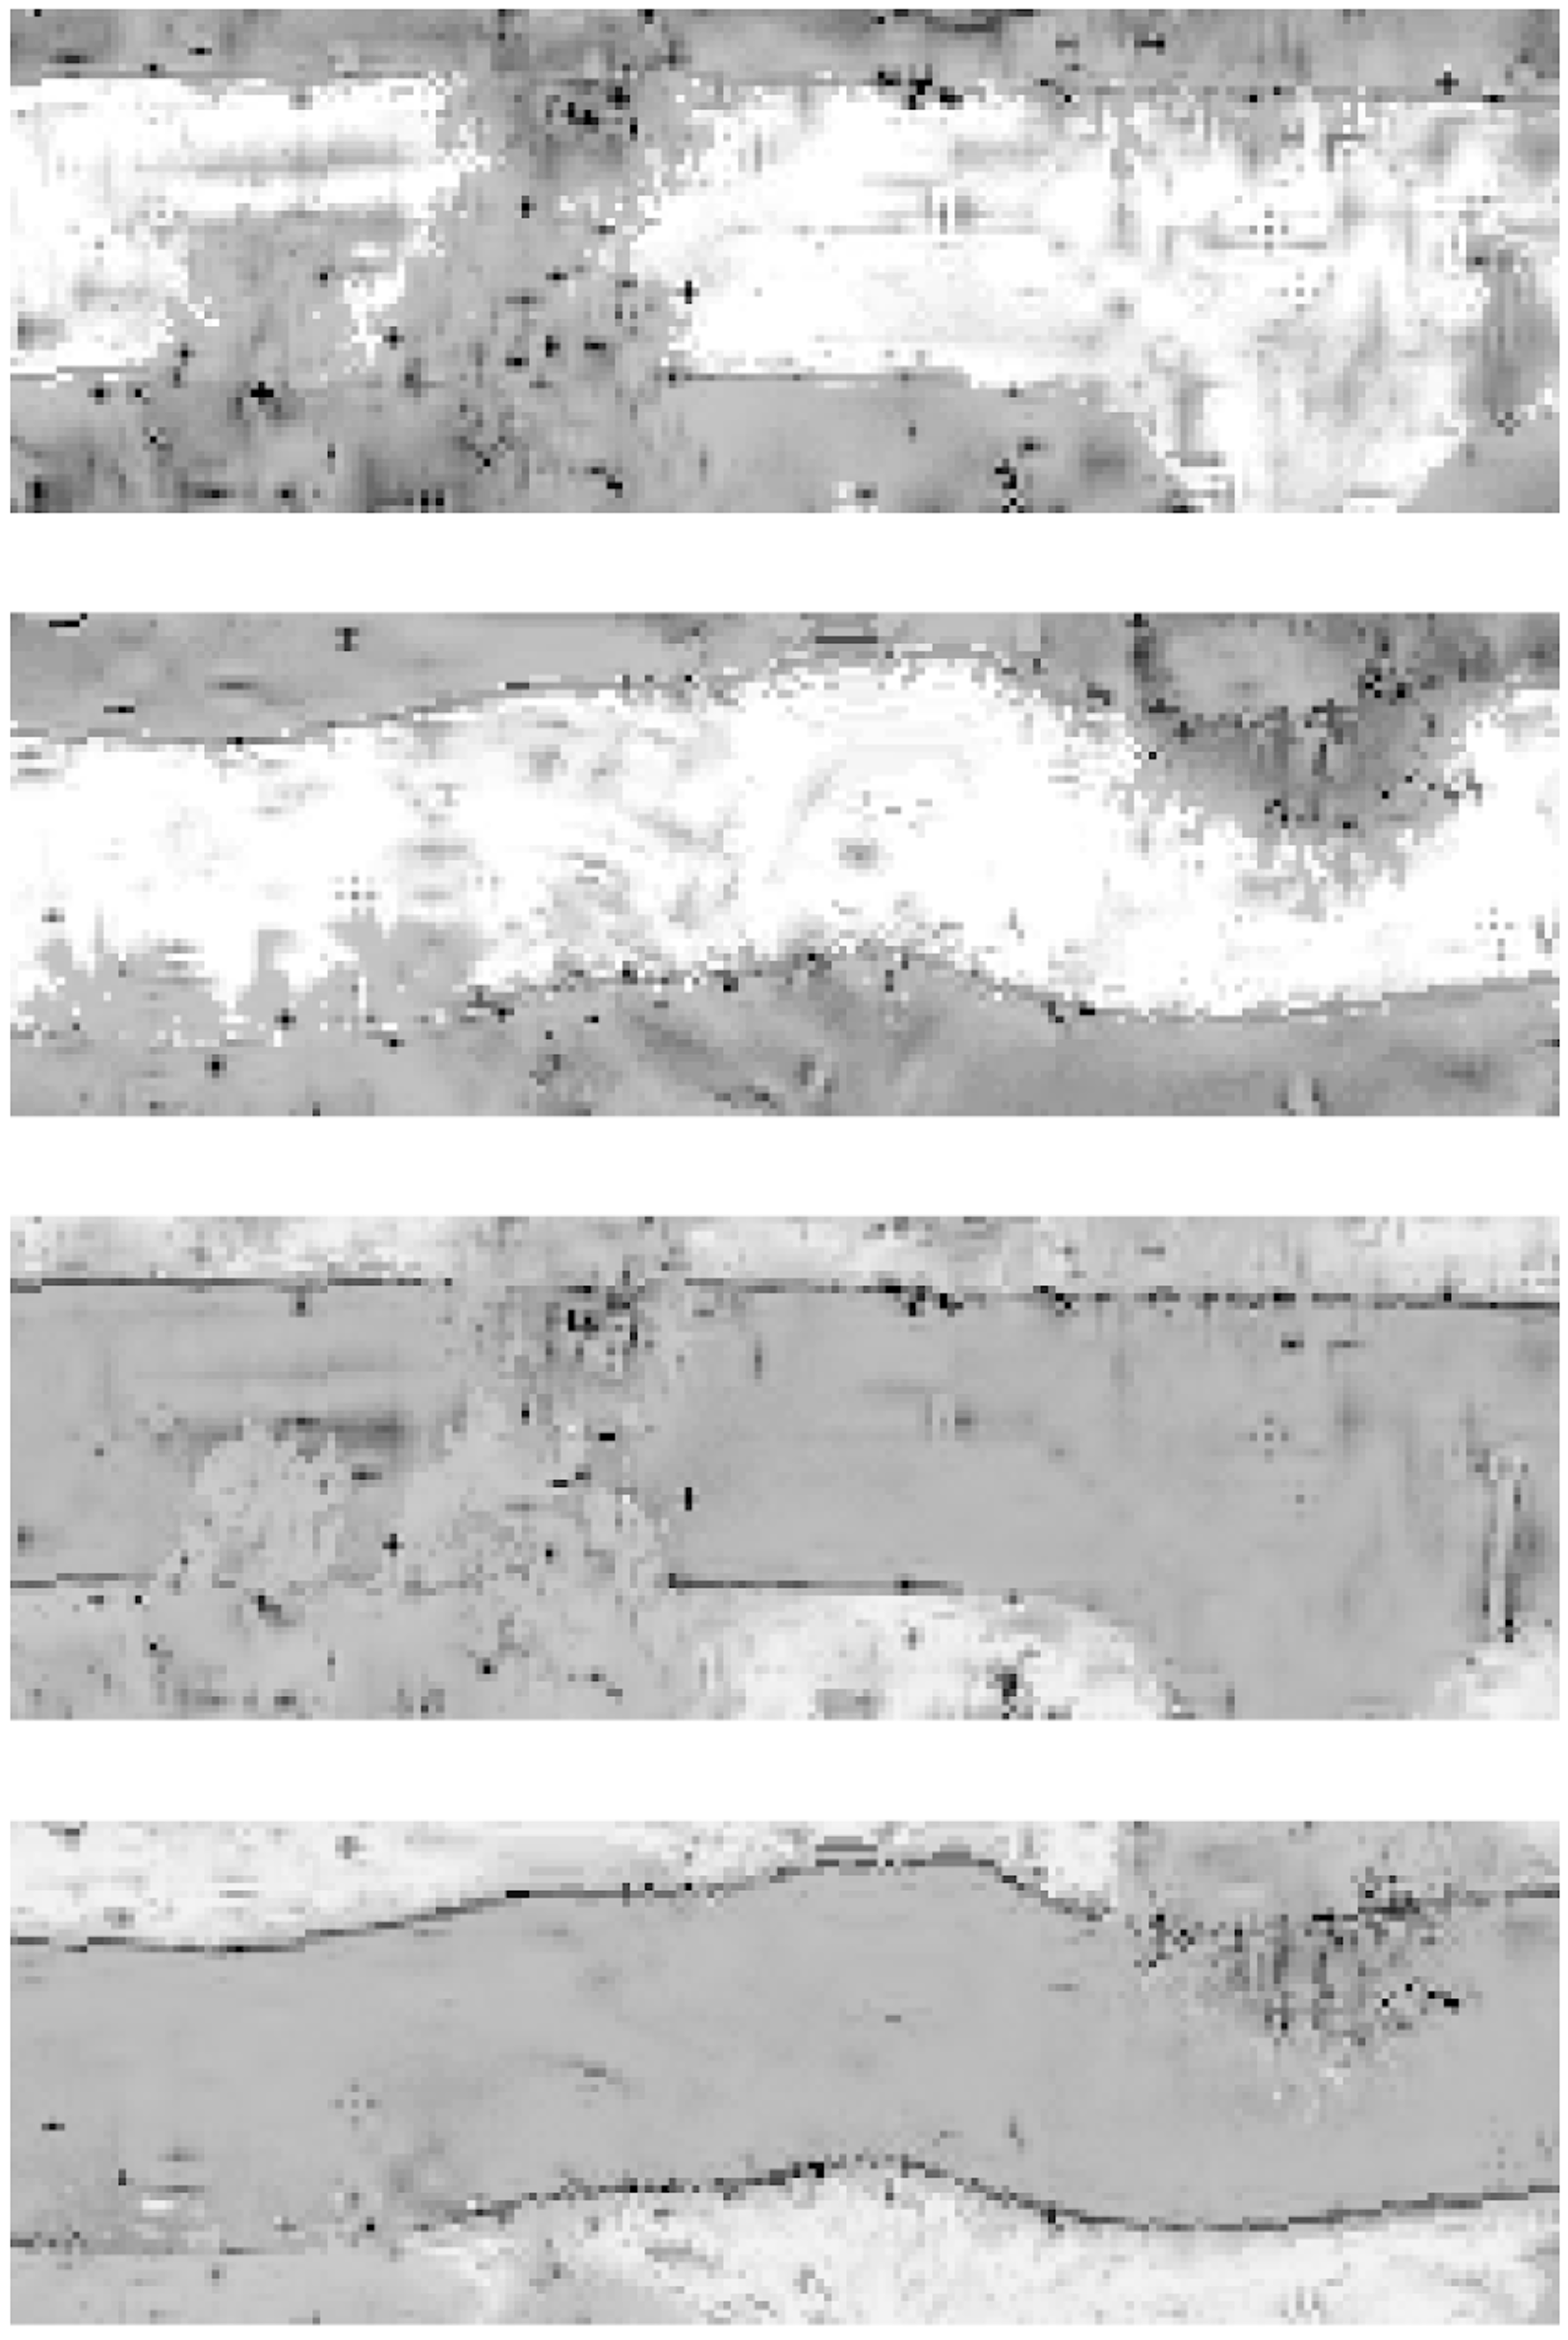
\includegraphics[width=0.75\columnwidth]{Figures/GMM_sample6.png}
    \caption[\ac{GMM} Result 2]{Example of GMMs on sample sidewalk. Row 1 and 2 shows the foreground GMM for sample sidewalk, and row 3 and 4 shows the back-ground for simple sidewalk. We use grey-scale to show the changes of probabilities, where for foreground, white is more likely to be sidewalk, and black is not.}
    \label{fig:GMM_result_2}
\end{figure}

We do not in general have a reliable estimate for the initial radius of our ribbon, 
but we can construct a trimap (\figref{fig:ribbon_3d}, bottom), as is done by \GrabCut{}, in order to estimate $\theta$. We choose a distance $\MaxDistance$ and numbers $\MinRadius < \MaxRadius$ 
so that all pixels with a distance of $[0, \MinRadius)$ are likely part of the ribbon (positive), all pixels within a distance of $[\MinRadius, \MaxRadius)$ are unknown, and others are are assumed not to be part of the ribbon (negative); 
In our experiments we chose  $\MaxRadius$ as twice the expected mean width of ribbons (e.g. 2 meters), $\MinRadius = \MaxRadius/2$, and $\MaxDistance=\MaxRadius+\MinRadius$.  
In figure \ref{fig:ribbon_3d} these regions correspond to strips of pixels in $\RibbonImage{}$ along the edges and center of the image.

% \begin{figure}[h!]
%     \centering
%     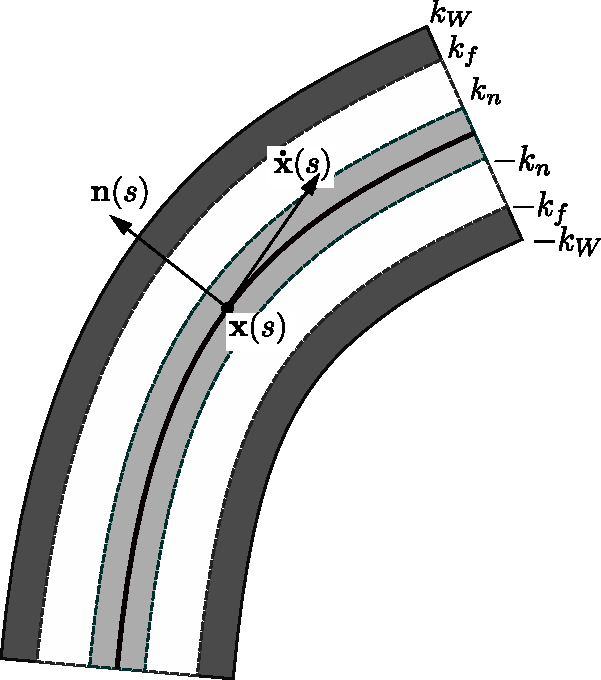
\includegraphics[width=0.3\textwidth]{Figures/sw-figure.pdf}
%     \caption[2D Ribbon Image]{A demonstration of the parameters for a ribbon in 2D, where $k_n$ indicates a lower-estimate for the radius of the ribbon, $k_f$ is an upper estimate, and $k_W$ is the maximum width of the ribbon image.}
%     \label{fig:2d_ribbon}
% \end{figure}

We use the EM-GMM algorithm to find a max-likelihood estimate of $\theta$ as a pair of Gaussian mixtures so that $\Pr(\phi|\text{pos}, \theta)$ is a mixture of four multivariate Gaussian functions and $\Pr(\phi|\text{neg}, \theta)$ is a mixture of eight; then $\Pr(\text{pos}|\phi, \theta)$ can easily be found using Bayes theorem as 
$$\Pr(\text{pos}|\phi, \theta)= \frac{\Pr(\phi|\text{pos}, \theta)}{\Pr(\phi|\text{pos}, \theta)+\Pr(\phi|\text{neg}, \theta)}.$$



%\FloatBarrier

The resulting probabilities are illustrated in \figref{fig:GMM_result_2}; we observe that even a coarse initial trajectory is usually enough to learn a more detailed, but noisy, estimate for the foreground object shape. However colors alone are not able to discriminate between occlusion and camouflage regions (such as the driveway in \figref{fig:GMM_result}). For rotational convenience we let $p[i,j]=-\lg \Pr(\text{pos}|\RibbonImage{}[i,j], \theta)$ and $q[i,j]=-\lg \Pr(\text{neg}|\RibbonImage{}[i,j], \theta)$; then the \ac{NLL} of a ribbon is proportional to a sum of $p[i,j]$ for all $i,j$ within the ribbon and $q[i,j]$ for all $i,j$ outside the ribbon. The aim of our \ac{DP} solution is to simultaneously optimize the probability based on color and shape of a ribbon-like feature. 


\section{A Dynamic Programming Algorithm}

We take $\RibbonImage{}$ as an input ribbon image with $m$ rows and $n=2\MaxDistance+1$ columns; $\RibbonImage{}{[i,j]}$ is a pixel in the image. We have an estimate $\Pr(\text{pos}|\RibbonImage{}_{[i,j]}, \theta)$ which we abbreviate as $p_{[i,j]})$. In addition there is some small set of allowed perturbations $\delta=\{(\delta_j, \delta_k)\}$ where $\delta_j$ is a change in direction and $\delta_k$ is a change in the radius of the ribbon. Each perturbation has a probability $\Pr(\delta_j, \delta_k)$ that controls the shape of the curve; in our experiments we use $\delta_j\in\{-1,0,1\}, \delta_k\in\{-1, 0,1\}$ in order to ensure that results are connected, and  $\Pr(\delta_j, \delta_k)=\Pr(|\delta_j|)\Pr(\delta_k)$ is two independent multinomial distributions which require only three parameters due to symmetry and because probabilities sum to unity. We can interpret $c_\mathit{bend}=-\lg \Pr(\delta_j=\pm1)$ as a penalty for bending the curve, and $c_\mathit{shrink}=-\lg \Pr(\delta_k=-1)$ as a penalty for shrinking the radius, or $c_\mathit{expand} = -\lg \Pr(\delta_k=1)$ as a penalty for expanding the radius of the curve. 

We visualize the problem of finding a ribbon as one of choosing a three-dimensional path through a scale-space where the first two dimensions represent locations of the ribbon's center, and the third dimension represent the thickness of the ribbon as illustrated in \figref{fig:ribbon_3d}. Every ribbon must start at one end of the image and follow a three-dimensional path through scale-space to reach the other end one slice at a time. Each slice corresponds to a row of the ribbon image and a point at location $(j, k)$ in the slice partitions the row into negative regions $(0\twodots{}j-k-1)$ and $(j+k+1\twodots{}n)$ with a positive region at $(j-k \twodots{} j+k)$ with thickness $2k+1$. The likelihood of any location $(j, k)$ is the product of the probabilities that each pixel on the same row belongs to the corresponding positive or negative regions.  In fact the probability is exponentially related to the size of each pixel; if one were to increase the resolution by a factor of $r$ then the contribution of each pixel would be raised to the power of $\frac{1}{r}$ so that the product would stay constant. In order to make our parameters invariant to scale, we divide the \ac{NLL} by $\MaxDistance{}$ when estimating the likelihood of a given $(j,k)$. 

We model the probability of a ribbon as the product of the probability of each location $(i, j, k)$ along the path times the probability of each edge from slice $i$ to slice $i+1$. We use dynamic programming to search to a path that minimizes the \ac{NLL} (the cost) of a path in procedure \proc{Segment-Ribbon}.

The pseudocode can be interpreted as follows: Line \ref{li:loop-slices} iterates through each slice of the ribbon image. Line \ref{li:loop-radius} iterates through all possible radii and line \ref{li:loop-center} explores all possible ribbon-centers from left to right. We use a variable $s$ to calculate \ac{NLL} of a set of regions as the ribbon shifts from left to right. If this is not the first slice, then line \ref{li:min-from-pred} selects the least-expensive (most probable) path that leads to location $(i, j, k)$ in the scale space.  At each step on pixel toggles from negative to positive, and one toggles from positive to negative as $s$ is updated in line \ref{li:update-s}.  We return the costs as well as the final offset and scale $(j^*, k^*)$ of the best path. 


\begin{codebox}
\Procname{$\proc{Segment-Ribbon}(\RibbonImage{})$} \label{alg:segmet-ribbin}
\li $p[i,j]\gets -\lg \Pr(\RibbonImage{}[i,j])/\MaxDistance{}$, 
          \hspace{2ex} $q[i,j] \gets -\lg \Pr(1-\RibbonImage{}[i,j])/\MaxDistance{}$
\li $C{[0\twodots{}m, 0\twodots{}n, 0\twodots{}n]} \gets \infty$
\li \For{$i \gets 0 \To m$} \Do                                                \label{li:loop-slices}
\li     \For $k \gets 0 \To \lfloor n/2 \rfloor $ \Do                          \label{li:loop-radius}
\li         $s = \displaystyle{\sum_{j=0}^{2k} p[i,j] +\sum_{j=2k+1}^n  q[i, j] }$
\li         \For $j \gets k \To n-k$ \Do  \label{li:loop-center}
\li              \If $i > 0$  \Do                                              \label{li:if-has-pred}
\li              $v \gets s {+}\displaystyle{\min_{\delta_j, \delta_k}\left(  
                              \begin{aligned}
                              C[i{-}1,j{+}\delta_j,k{+}\delta_k] \hspace{3ex}\\
                              \hfill{}-\lg \Pr(\delta_j, \delta_k)
                              \end{aligned}
                            \right)}$  
                               \label{li:min-from-pred}
\li              \Else $v\gets s$
                 \End
\li              $C{[i, j, k]} \gets v$                                       \label{li:dp-store}
\li              $s \gets s{+}q[i,j{-}k]{-}p[i, j{-}k]{+}p[i, j{+}k]{-}q[i,j{+}k]$ \label{li:update-s}
           \End
       \End
    \End
\li $j^*, k^* \gets \displaystyle{\arg\min_{j,k} C{[m, j, k]}}$
\li \Return $C, j^*, k^*$
\end{codebox}

The \proc{Backtrack-Ribbon} algorithm selects the least-costly (most probable) ribbon and it is copied into to $T$ and $R$; so that the most likely path has scale-space coordinates $(i, T[i], R[i])$ for $i=0\twodots{}m$. 



\begin{codebox}
\Procname{$\proc{Backtrack-Ribbon}(C, j^*, k^*)$} \label{alg:backtrack-ribbon}
\li $T{[0{\twodots}m]} \gets 0$, \quad $R{[0{\twodots}m]} \gets 0$             
\li $T{[m]}, R{[m]} \gets j^*, k^*$ \label{li:backtrack-best-last}
\li \For $i \gets m-1 \Downto 0$ \Do
\li      $\delta_j, \delta_k = \displaystyle{\arg\min_{\delta_j,\delta_k}C{[i,j{-}\delta_j,k{-}\delta_l]}{-}\lg \Pr(\delta_j,\delta_k)}$
\li      $T{[i]}, R[i] \gets T{[i+1]}-\delta_j, R{[i+1]}-\delta_k$                                                 \label{li:backtack-choose-pred}
    \End
\li \Return $T, R, C_{[m, j^*, k^*]}$
\end{codebox}


If one wishes the path to be connected in scale-space, then there are only $3\times3$ possible values for $\delta_j, \delta_k$ in line \ref{li:min-from-pred}; so the algorithm is $\Theta(m n^2)$ and used $O(m n^2)$ space, where $m$ is the length of a ribbon and $n=2\MaxDistance+1$ is the maximum thickness of a ribbon. Since $\MaxDistance$ is typically a constant, this algorithm is effectively linear on the length of a ribbon.
\chapter{Preliminary Result}

A four-step adopt approach for sidewalk segmentation was developed. Locating sidewalk geometric information from raw \ac{VHR} data would be the first step, then generating ribbon image on each sidewalk which has been locate in the map data. After that, adopting density estimation on each pixel in ribbon image which generated from last step. Finally, we applied dynamic programming algorithm with fully developed penalty function to get edges on both side of sidewalks, then just simply converted the ribbon image back to it's original shape.

\section{Sidewalk Geometric Information Locator}

Before using deep learning network to determine sidewalk's location, hand marking all sidewalk from imagery or extract the geometric information of each sidewalk from resources like \ac{OSM} was required. It's challenging since the geometric accuracy was not precise, which could cause performance issue due to the fact that we relied on this information to segment the sidewalk part from maps for the next step. To ensure data accuracy, we spent days marking all sidewalks and their precise boundaries in Arizona Central. We can located each sidewalk by using the geometric information and saved them into separate files. We also calculated the average sidewalk width from boundaries to decide reasonable window size in the following step.

\section{Ribbon Image Generation}

\begin{figure}
    \centering
    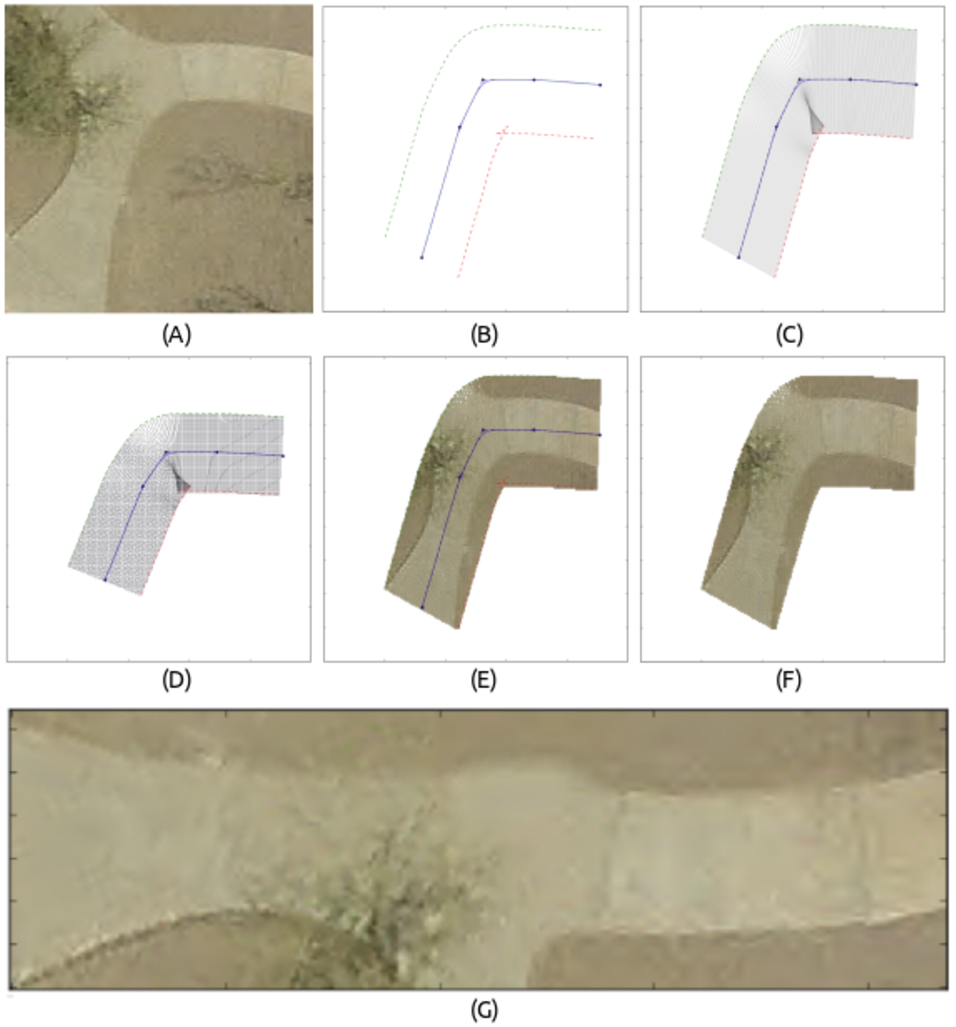
\includegraphics[width=\textwidth]{Figures/straghten.pdf}
    \caption[Ribbon Image Generation]{Ribbon image generating process: from sub-figures A to G, we showed the step by step process to generate ribbon-image from a partial sidewalk. From raw input (A), we smoothed mid line and generated parallel off-site (B). Generated pixels (C) and connected each pixel to its correspond color data from the raw input (D). After gathered pixel data (E), we removed mid-line (F) and generated the ribbon image(G).}
    \label{fig:StraightenProcess}
\end{figure}

\begin{figure}
    \centering
    \includegraphics[width=0.95\textwidth]{Figures/sample2_demo.png}
    \caption[Sample Sidewalk 2]{A ribbon image straighten output on sample sidewalk, row 1 shows the original input, row 2 to 5 show the ribbon image output separate into parts.}
    \label{fig:Sample_Sidewalk_2}
\end{figure}

To apply the hypothesis, we develop a way to convert the given sidewalk into a ribbon image. As shown in figure \ref{fig:StraightenProcess}, first, we used the previous outcome (A) from the last step as input and connected all coordinate points data as the mid-line for the sample sidewalk, then we applied a smooth function that we created to smooth the mid-line, so the mid-line shape would fit better to the actual sidewalk shape(B). We generated two parallel line as offsets on each side of the mid-line with a distance of twice the average width in between. So ideally even the mid-line was not perfectly laying on the middle, we could still fit the whole sidewalk into the ribbon image. For each point on the mid-line, we connected the corresponding points on both offsets to get the movement of the sidewalk and recorded them(C, D), we could generate the straightened ribbon image using the color data from each pixel in the points set that we record earlier(E). The image data just in between each offset, with constant image width could be retrieved after that(F). Reshaping the image data was needed to generate the ribbon image(G). Figure \ref{fig:Sample_Sidewalk_2} shows the complete ribbon-image output result on sample sidewalk. We separate it into parts to show better detail. 

\section{Density Estimation on Pixels}

Before moving on to dynamic programming approach, each pixel need to be given a initial score to classify each pixel is sidewalk or not. To achieve that, as shows in figure \ref{fig:GMM_Sample_2}, we applied a density estimation function to find the probability for each pixel in the ribbon image. For foreground, we used grey-scale to determine the probability likely-hood for the sidewalk-feature, where white is more likely to be sidewalk and black is less likely. The background is the other way around, which made black is more likely to be sidewalk and white is not.

\begin{figure}[H]
    \centering
    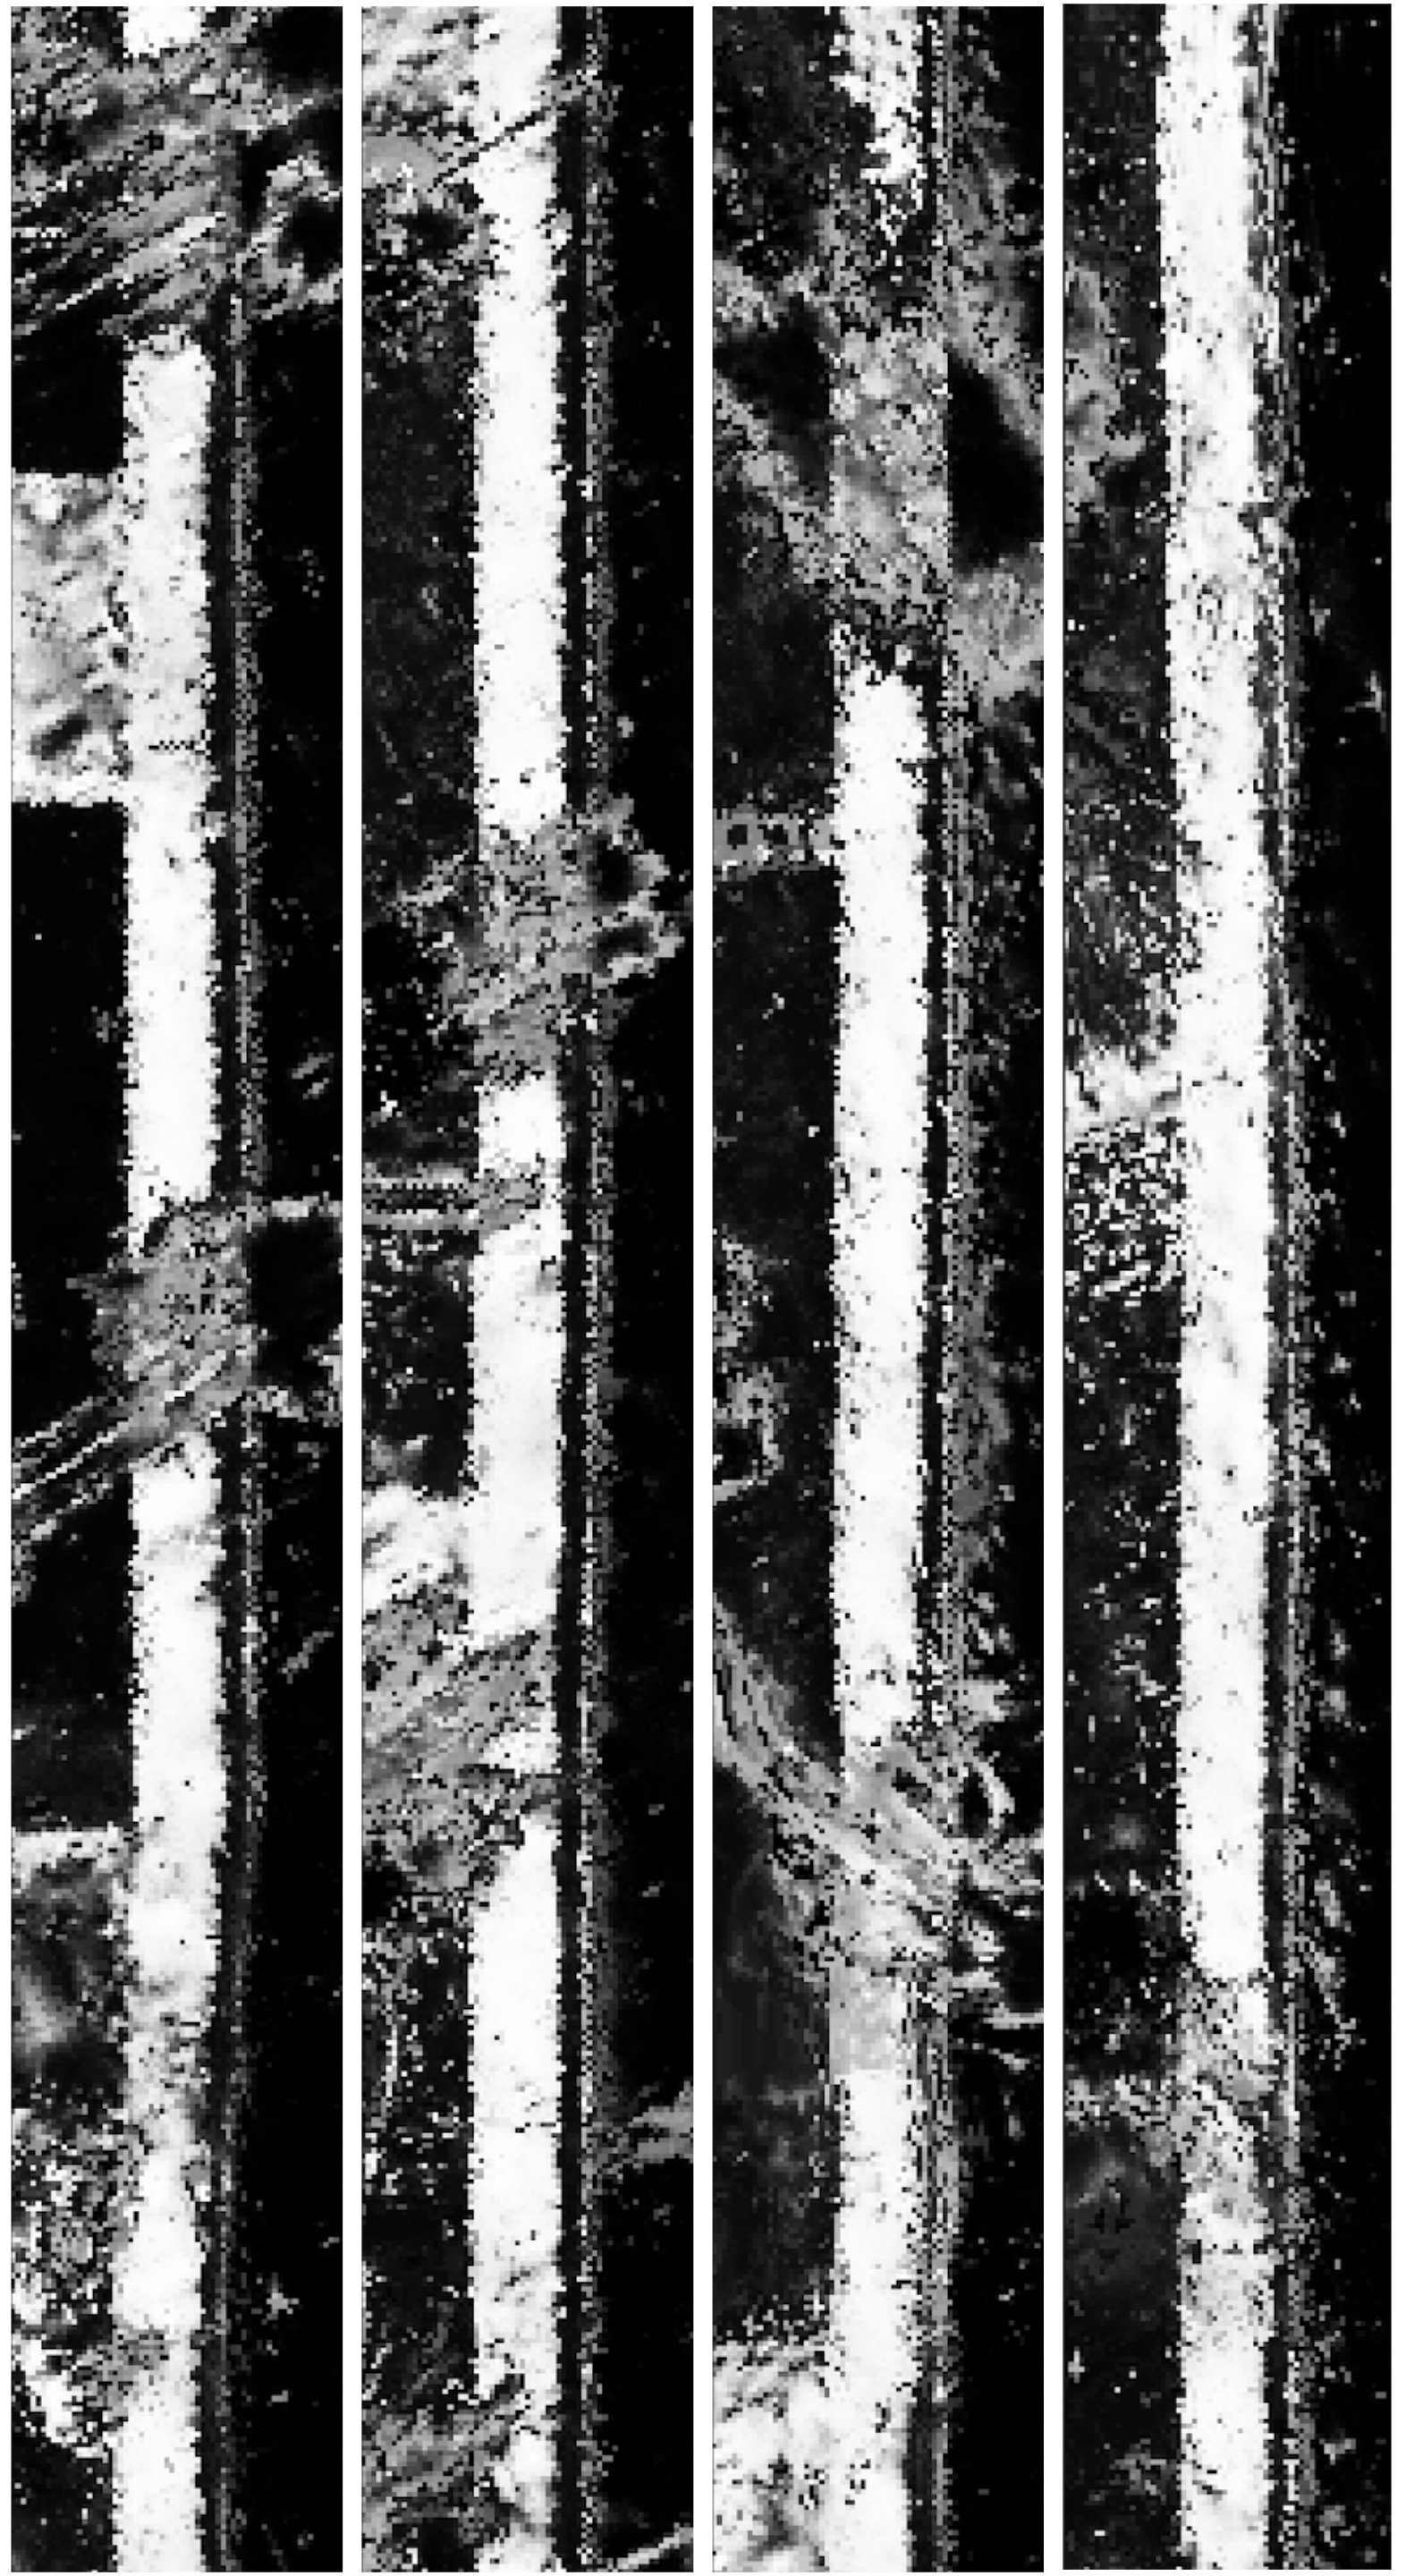
\includegraphics[width=0.65\textwidth]{Figures/GMM_SAMPLE2.png}
    \caption[Density Estimation on Sample Sidewalk]{A sample figure with density estimation applied on figure \ref{fig:Sample_Sidewalk_2}. Where white indicates pixels are more likely to be a sidewalk feature and black indicates pixels are more likely to be a non-sidewalk feature. We separate it into 4 parts from column 1 to 4.}
    \label{fig:GMM_Sample_2}
\end{figure}

\section{The Dynamic Programming Algorithm}

We used our dynamic programming algorithm on the ribbon image to find the max score for each pixel that had more probability to be sidewalk feature that we mentioned in Chapter 4. More importantly, we introduced a penalty control function that makes each horizontal movement in the edges or center cost more than vertical movement. Basically, for each line of pixels, if they think the edges or center should shift more horizontally than one pixel compares to the last line, we score them with more penalty. 

Figure \ref{fig:penalty} shows our algorithm managed to separate the driveway and sidewalk under the same feature as penalty increase. So we could apply the dynamic programming solution to locate the precise boundaries of given ribbon image. The penalty control improved our performance significantly. Because of this, our approach could predict the sidewalk under the tree shadow and other shadows or obstacles, which bring us more accurate result compare to other methods.

As shown in figure \ref{fig:sample_result2}, after we generate the result on ribbon image, just need to simply covert the ribbon image back to its original shape by reverse the method that generates the ribbon image. 

\begin{figure}[H]
    \centering
    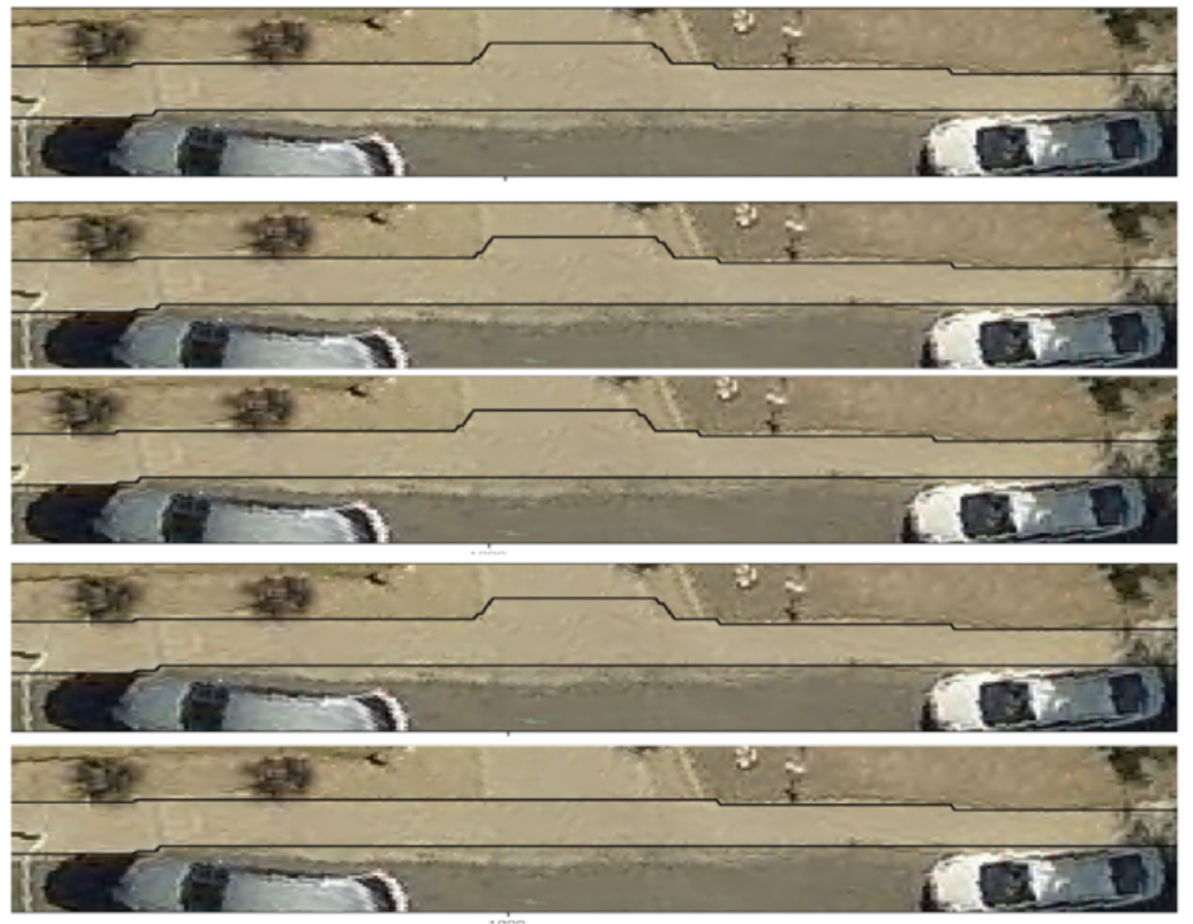
\includegraphics[width=\textwidth]{Figures/penalty.pdf}
    \caption[Penalty Process]{Comparison with penalty change, we tested a variety of variables to decide which variable had best performance for width control. With the penalty increased at a reasonable amount, our algorithm decided not to recognize a driveway as sidewalk walk, in order to keep the sidewalk width consistent, even though they are the same texture.}
    \label{fig:penalty}
\end{figure}

\begin{figure}
    \centering
    \includegraphics[width=0.95\textwidth]{Figures/sample2_result.png}
    \caption[Desire Output on Sample Sidewalk]{Detail demonstration on desire result after applying our dynamic programming approach. Where row 1 shows the result after reshape, row 2 to 5 shows the boundaries we calculated on ribbon image from \ref{fig:Sample_Sidewalk_2}.}
    \label{fig:sample_result2}
\end{figure}

\section{Result Evaluation}

We evaluate our results using precision ($P$), recall ($R$) and the balanced F-measure ($F_1$) defined as follows:
\begin{align}
     P &= \frac{\mathit{TP}}{\mathit{TP} + \mathit{FP}}, \\
     R &= \frac{\mathit{TP}}{\mathit{TP} + \mathit{FN}}, \\  
     F_1 &= \frac{2 P R}{P + R}
\end{align}
where 
\acp{TP} is the number of pixels correctly marked as positive, 
\acp{FN} is the number incorrectly marked as negative and 
\acp{FP} is the number incorrectly marked as positive. 

We compare our results against common segmentation approaches 
\ac{SLIC}~\cite{Achanta:149300}, \ActiveContours{}~\cite{ActiveContou09} and \GrabCut{}~\cite{Rother2004-ou} 
in Table~\ref{tab:quantitative-against-common} using a manually annotated region of 
Phoenix AZ. The test region was acquired as \ac{VHR} 4-inch aerial orthophotos, 
and manually annotated by drawing a polygonal outline. 
When a portion of the sidewalk was occluded or camouflage with the surrounding pavement 
(including gutters) we used our best judgment to connect the visible portions of the sidewalk. For all of of the examples we present, with figure \ref{fig:change_on_recall} that shows detail parameters evaluations, we set $c_\mathit{bend}=\frac{1}{2}, c_\mathit{shrink}=c_\mathit{expand}=2$ which were experimentally found to produce the best result. Note that in our implementation we did not take care to ensure that $\Pr(\delta_k)$ summed to unity, and instead assumed that $-\lg \Pr(\delta_k=0)$ was zero, which does not have a probabilistic interpretation but is more convenient for computation. 

\begin{table}[h!]
    \caption{Quantitative comparison. }
    \label{tab:quantitative-against-common}
    \centering
    \begin{tabular}{r ccc}
                            & $P$ & $R$& $F_1$ \\ 
                                 \hline 
                  \ac{SLIC} & 0.876 & 0.839 & 0.857 \\
          \ActiveContours{} & 0.873 & 0.866 & 0.869  \\
                 \GrabCut{} & 0.969 & 0.877 & 0.925  \\ 
                                 \hline
                \textbf{DP} & \textbf{0.973} & \textbf{0.961} & \textbf{0.967}   
    \end{tabular}
\end{table}

For qualitative comparison we compare against \ac{SLIC}, \ActiveContours{}, and \GrabCut{}, in
\figref{fig:Sample_4_compare}. The former presents a portion of a hiking trail in a desert region where the foreground and background materials are similar and the path curves and varies in thickness. The \ac{DP} approach is smooth and also follows the boundary of the path closely, and it also follows a reasonable trajectory where the path bifurcates. More challenging scenarios are shown in \figref{fig:Sample_2_compare} and \figref{fig:Sample_3_compare}, which includes examples of occlusion, shadow, and camouflage.  

\begin{figure}[H]
    \centering
    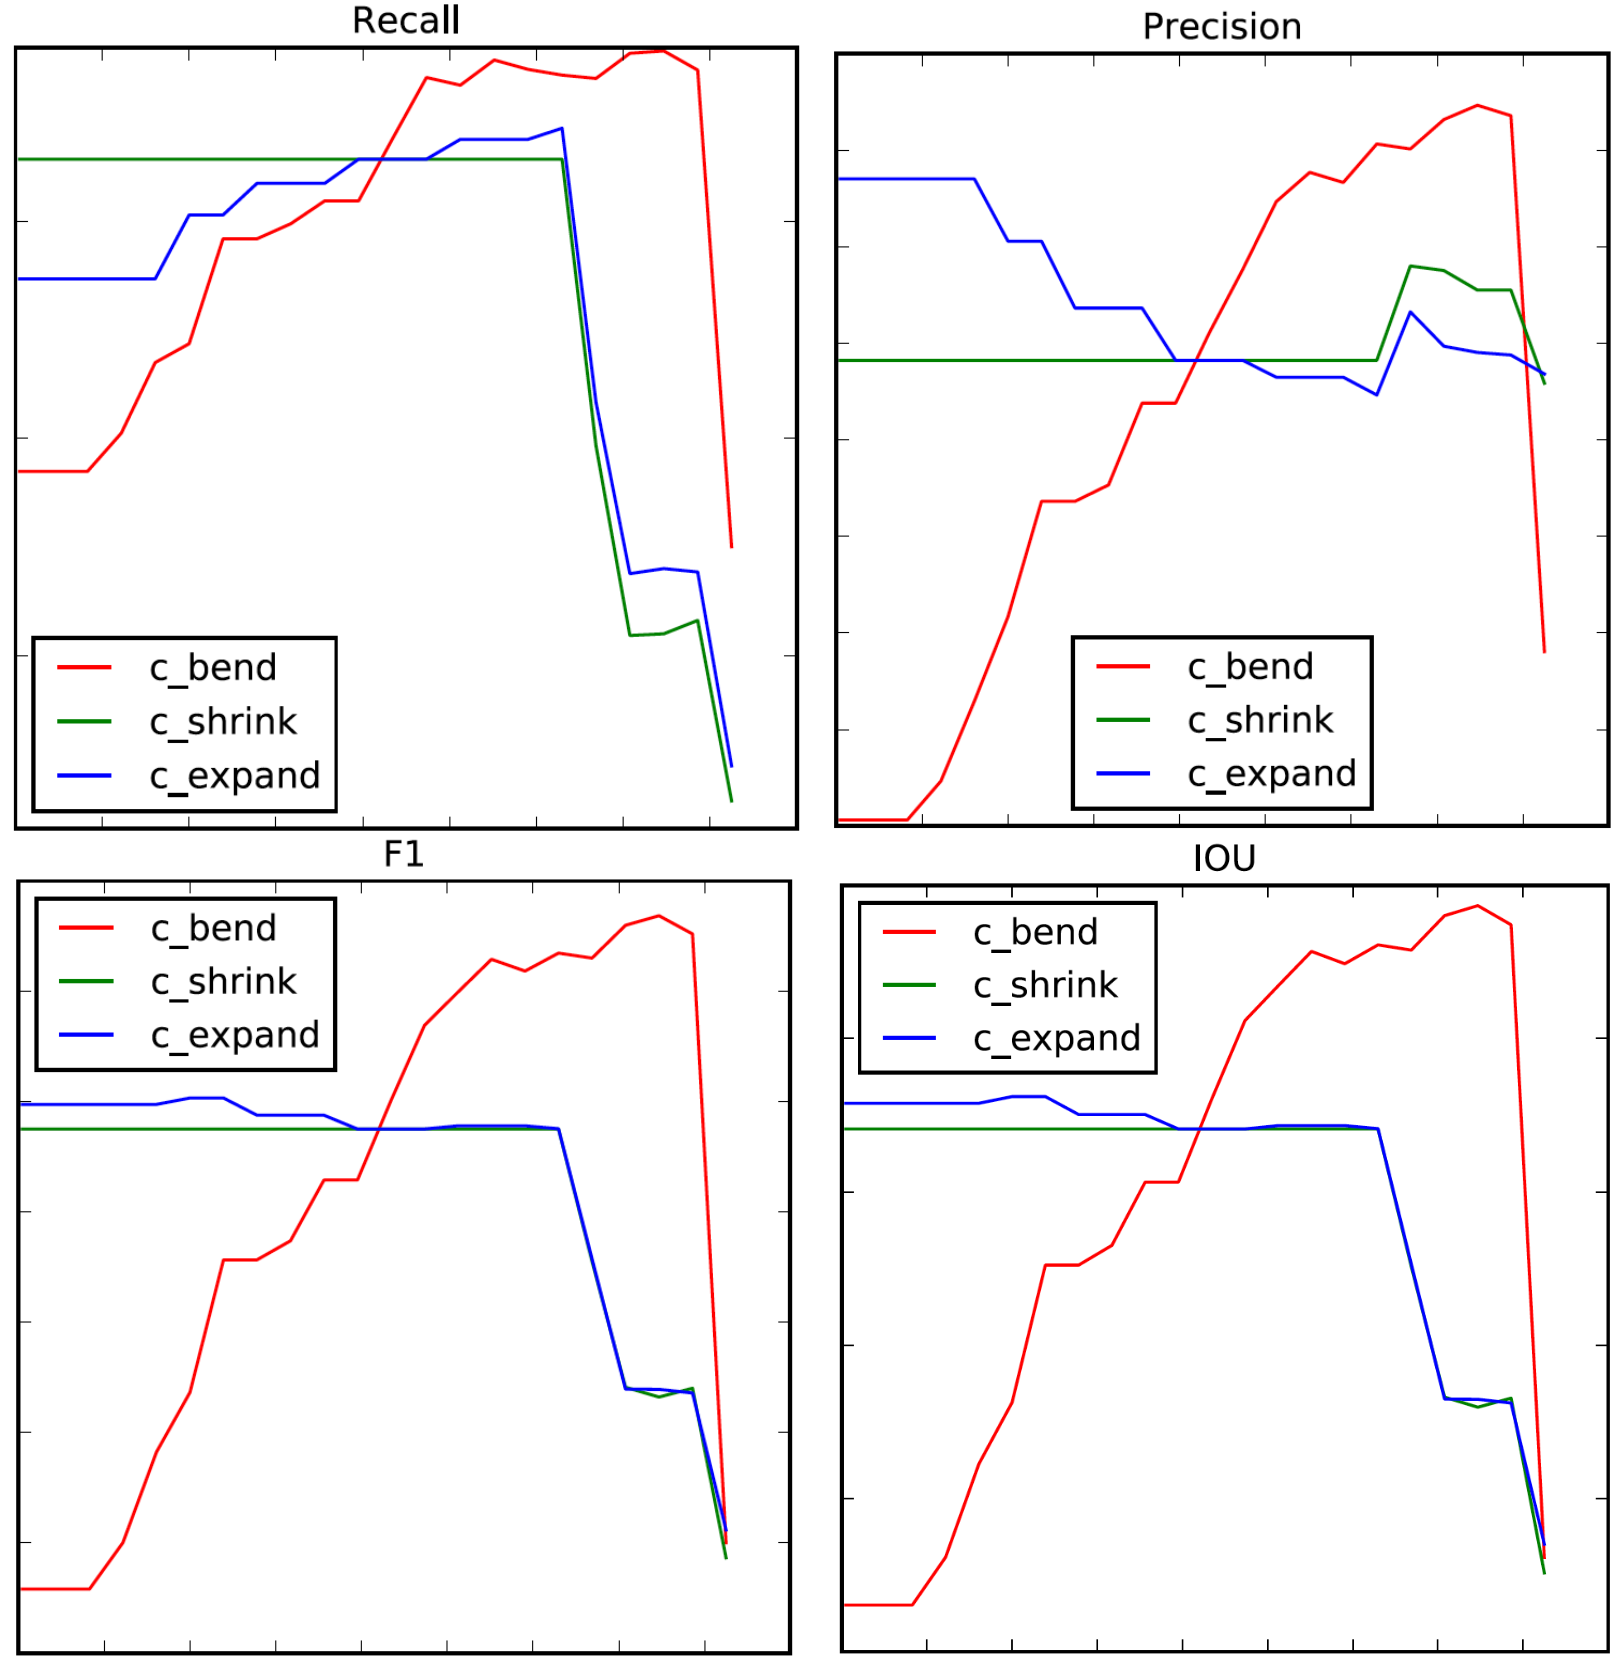
\includegraphics[width=0.95\textwidth]{Figures/changes_on_recall.png}
    \caption[Parameters Evaluation]{Detail comparison on $c_{bend}$, $c_{shrink}$ and $c_{expand}$. Where red line represent $c_{bend}$, green line represent $c_{shrink}$ and blue line represent $c_{expand}$. We generate these based on equations from Recall (6.2), Precision (6.1), F1 (6.3) and Intersection over Union.}
    \label{fig:change_on_recall}
\end{figure}

We have also identified the following limitations of the proposed method: it assumes that an initial ribbon overlaps with the feature in the corresponding orthophoto. We have not suggested an approach to determine if a walking path has been removed, or has been completely occluded. Furthermore, we assume \ac{VHR} orthoimagery that has enough resolution to build a model for colors on and off the ribbon. The proposed approach finds integer raddii, so thicknesses are all multiples of two. We recommend up-sampling images, which will allow the proposed approach to solve for a trajectory with sub-pixel precision. Finally, while we do make some assumptions when we select $\MinRadius{}, \MaxRadius{}, \MaxDistance{}$ the method as presented does not impose a prior on expected thickness of ribbons; often this is known and it could be used to generate plausible results for completely occluded ribbons.

We also test our approach in different cities. For initial trajectories, We pull the corresponding footway data from overpass-turbo \cite{overpass_turbo}. Finding map data is challenging since there not exist much \ac{VHR} imagery from public source. We use the imagery data form GIS government database and treat it as input map. \figref{fig:oxford1} demonstrate plausible result on a sidewalks heavy area, we randomly selected a few from Oxford, OH. Row 1 shows that our approach are able to find the precise boundaries under trees or building shadows, with less accuracy around intersection area. Except above from row1, row 2 also demonstrate the camouflage with adjacent material. We treat the intersection part as overlapping sidewalks, and process them individually. \figref{fig:ny1}, \figref{fig:ny2} and \figref{fig:ny3} show the random samples we select from New York area. Predicting is heavier involved in these area since some sidewalks are partially under tree leaves instead of just shadows. 

% \todo[TALK ABOUT OTHER CITY]

% We generated few results from our sample inputs to compare with other methods according to figure \ref{fig:Sample_4_compare} and mathematics feedback from table \ref{table:sample_4}. From above feedback, Grabcut had decent performance with recognized edges for given sidewalk, since it's false positive (Red) in figure \ref{fig:Sample_4_compare} is significantly small. The problem that mentioned in chapter 2 is still the main reason that it's result is less accurate than ours. In row 1, 2, 3, column 1 of figure \ref{fig:Sample_4_compare}, the grabcut is unable to segment sidewalks which under the tree shadows. For the same issue, in column 4, our result indicated that we could successfully recognize and get boundaries from sidewalk. Same with figure \ref{fig:Sample_2_compare}. In row 1, 2, 3, we compared the output from column 1 and column 4, which are the outputs from grabcut and our approach. It's clear that our approach can successfully segment sidewalk when it connects with drive way (column 1), or there's obstacle (column 3) exist, not only for tree shadows. Also, another advantage of our algorithm is that our approach can segment sidewalks from gutters. We believe other methods are not able to recognize gutter under any circumstances. 

\begin{figure}
    \centering
    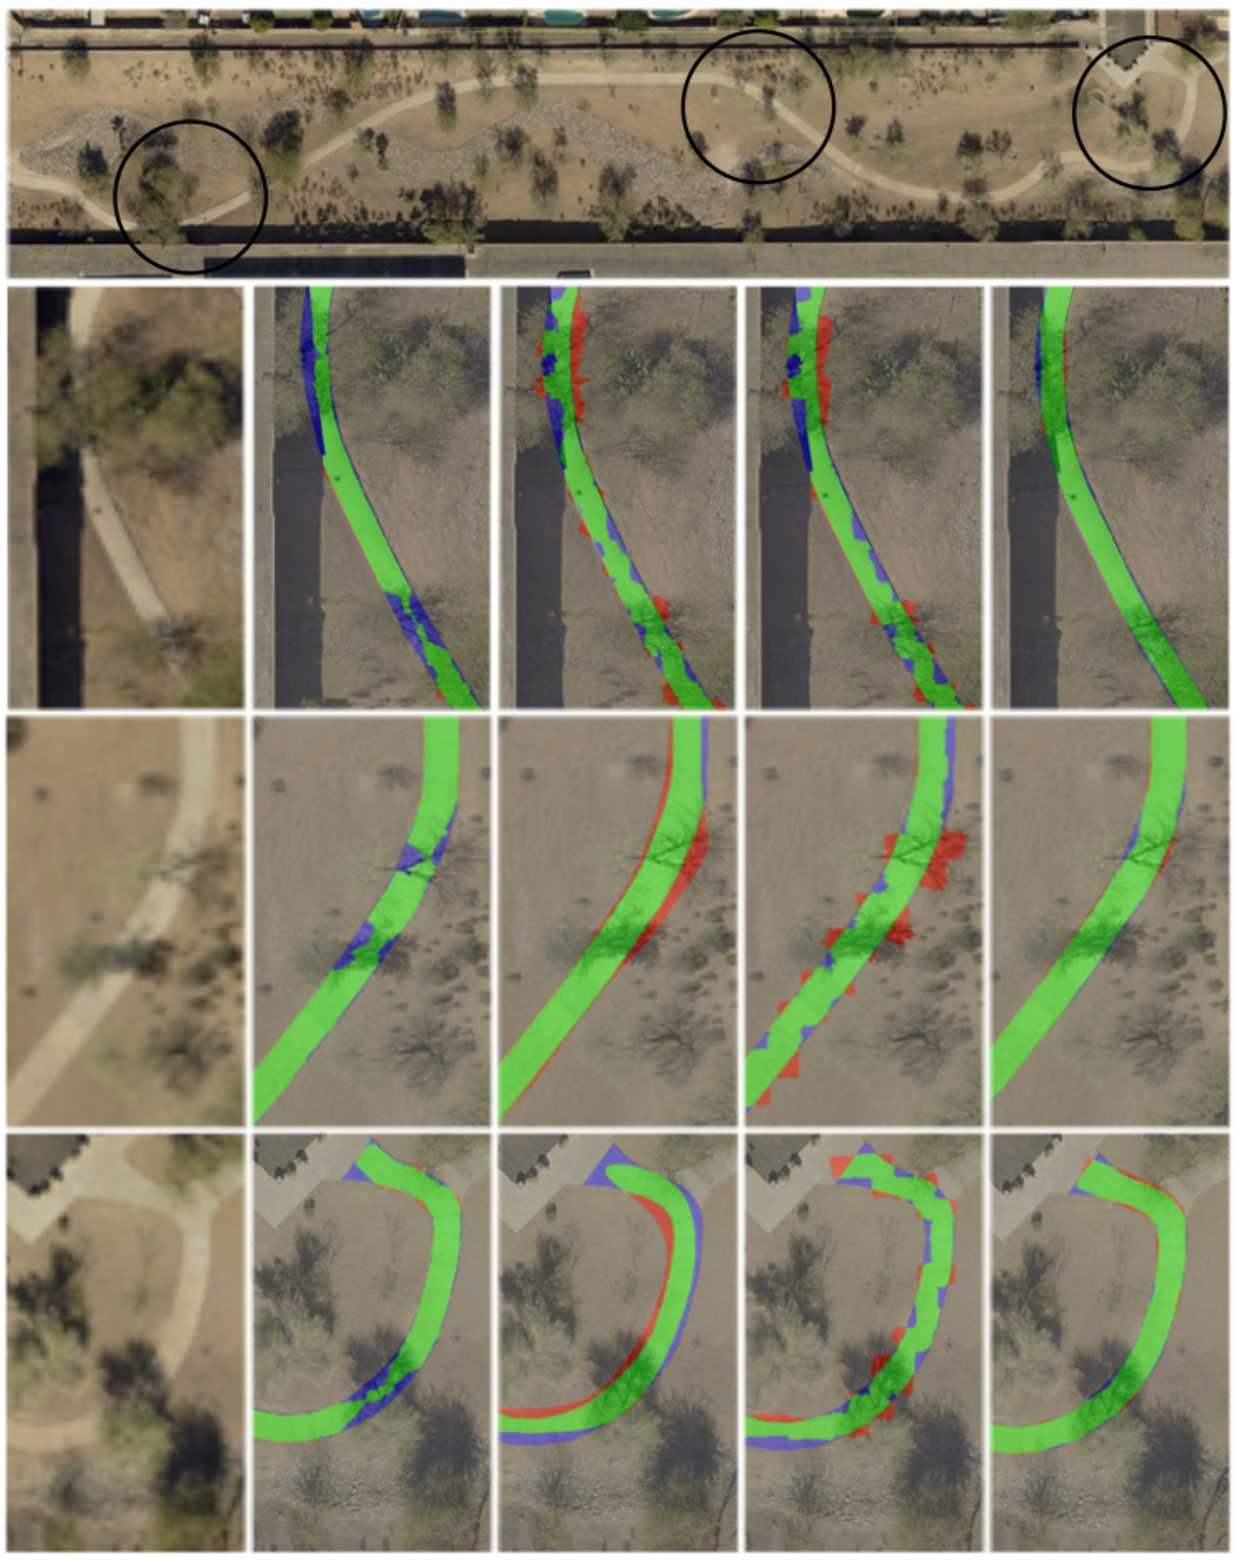
\includegraphics[width=0.9\textwidth]{Figures/4_comparison.pdf}
    \caption[Methods Comparison on Sample Sidewalk 1]{A sample result compared with three different methods and ours. In the order of grabcut, slic, active Contours and ours from left to right. Grabcut is unable to separate the tree shadow from actual sidewalk feature, same with slic and active contours. Our results are more likely to predict the accurate edges under obstacles.}
    \label{fig:Sample_4_compare}
\end{figure}

% \begin{table}[h]
% 	\centering
% 	\begin{tabular}{ | c | c | c | c | } 
% 		\hline
% 		Methods	& TP-FP\% & TP\% & FP\% \\
% 		\hline
% 		Grabcut			& 86.10\% & 87.69\% & 1.82\% \\
% 		\hline
% 		Slic			& 73.90\% & 83.88\% & 11.90\% \\
% 		\hline
% 		Active Contour	& 75.70\% & 86.63\% & 12.63\% \\
% 		\hline
% 		Ours            & 93.48\% & 96.06\% & 2.69\% \\
% 		\hline
% 	\end{tabular}
% 	\caption{Mathematics result comparison between our result and others from figure \ref{fig:Sample_4_compare}}
% 	\label{table:sample_4}	
% \end{table}

\begin{figure}
    \centering
    \includegraphics[width=0.78\textwidth]{Figures/sample_sidewalk_1.png}
    \caption[Methods Comparison on Sample Sidewalk 2]{A sample results compared with three different methods and ours. In the order of active Contours, grabcut, slic, ours from left to right. Which shows samples of separating drive way and gutters.}
    \label{fig:Sample_2_compare}
\end{figure}

\begin{figure}
    \centering
    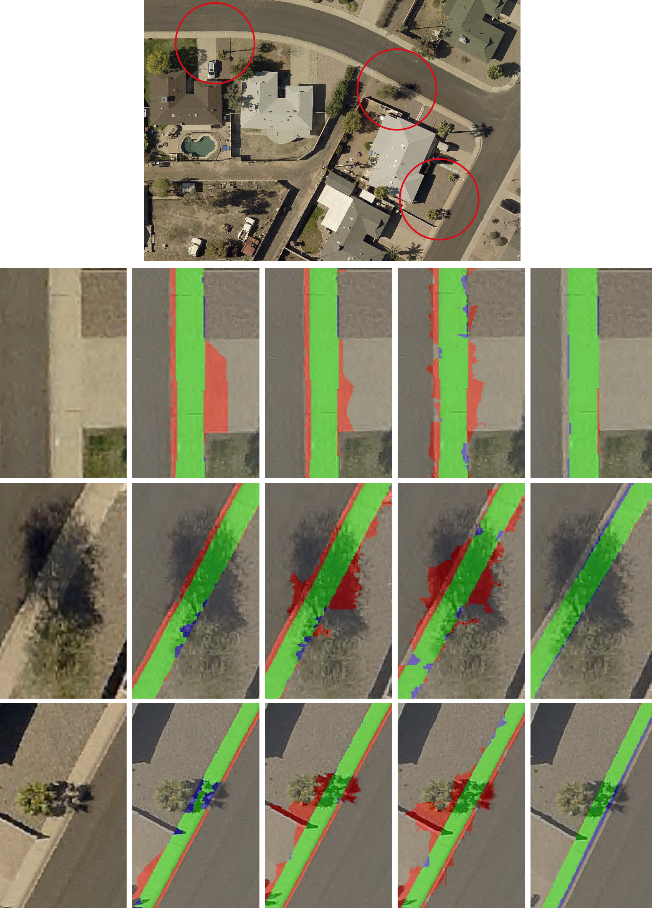
\includegraphics[width=0.86\textwidth]{Figures/2_comparison_needed.png}
    \caption[Methods Comparison on Sample Sidewalk 3]{A sample results compared with three different methods and ours. In the order of grabcut, slic, active Contours, ours from left to right. Which shows samples of separating drive way and gutters.}
    \label{fig:Sample_3_compare}
\end{figure}



\begin{figure}
    \centering
    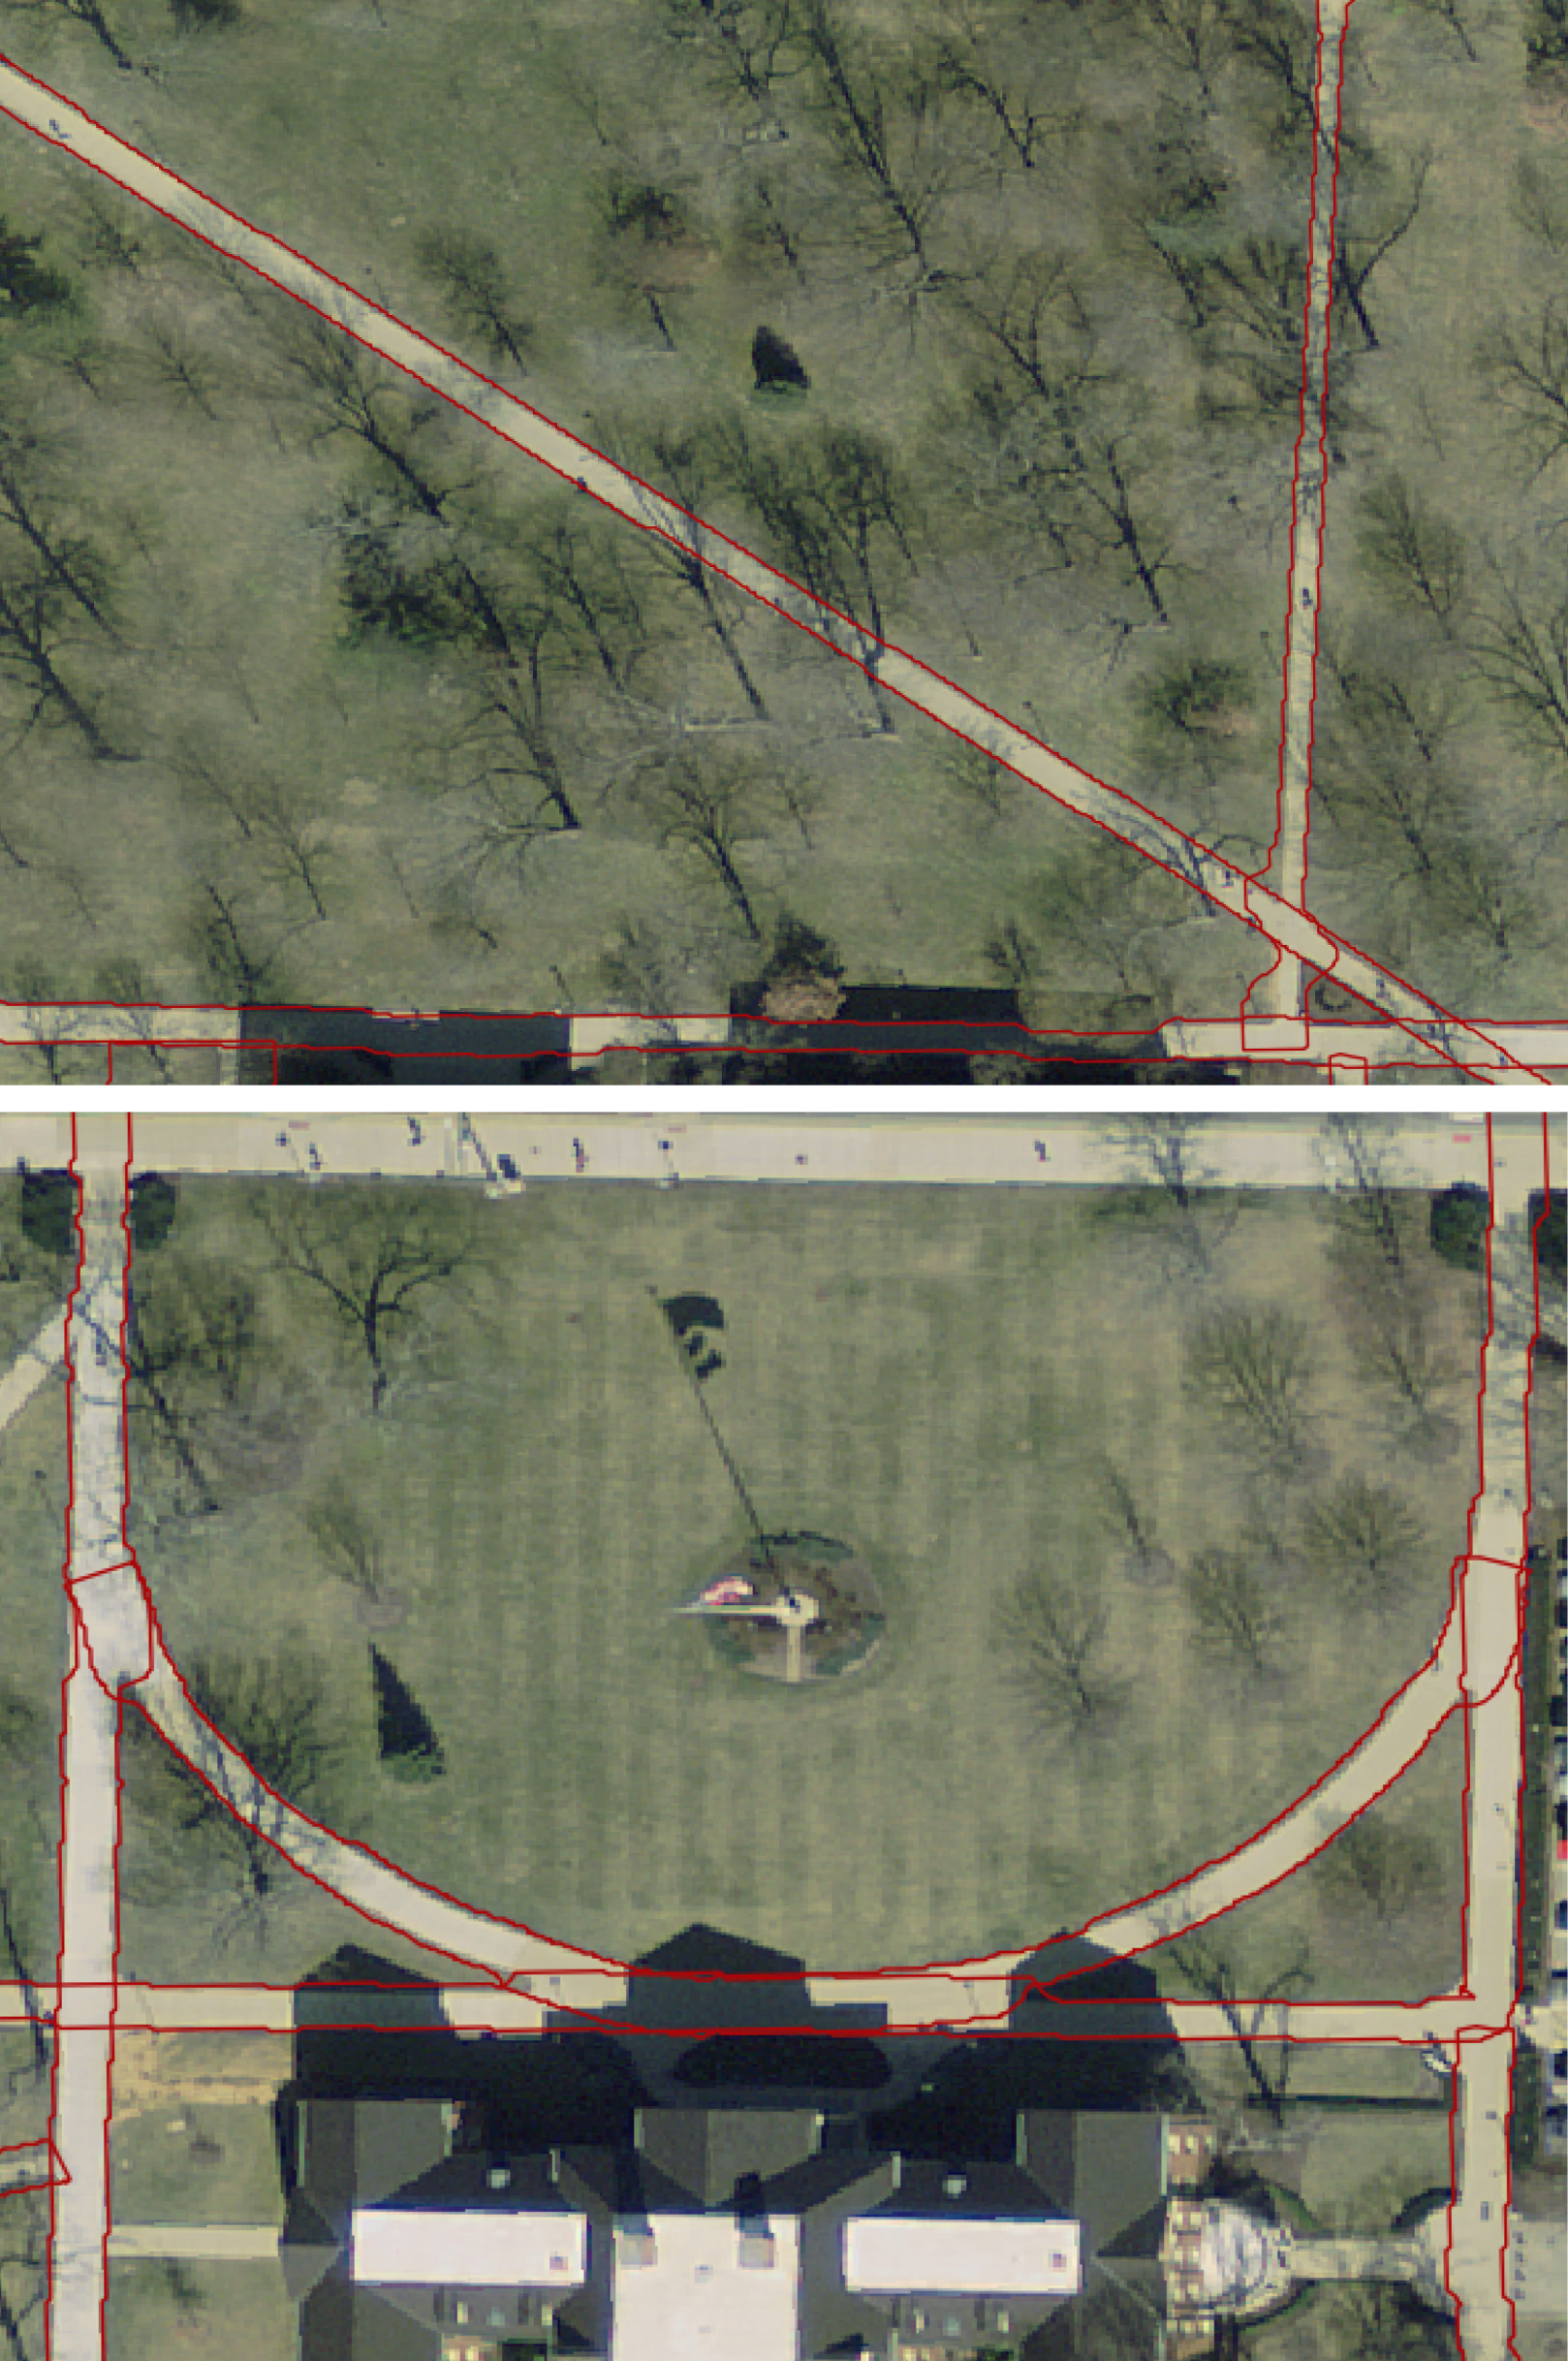
\includegraphics[width=0.8\textwidth]{Figures/Oxford_success_complex.png}
    \caption[Sample Sidewalk 3]{Demonstration on sample sidewalks with our approach. We use Oxford Area that include more complex sidewalks. It shows that given samples are able to separate trees, building shadows and camouflage with adjacent materials.}
    \label{fig:oxford1}
\end{figure}

\begin{figure}
    \centering
    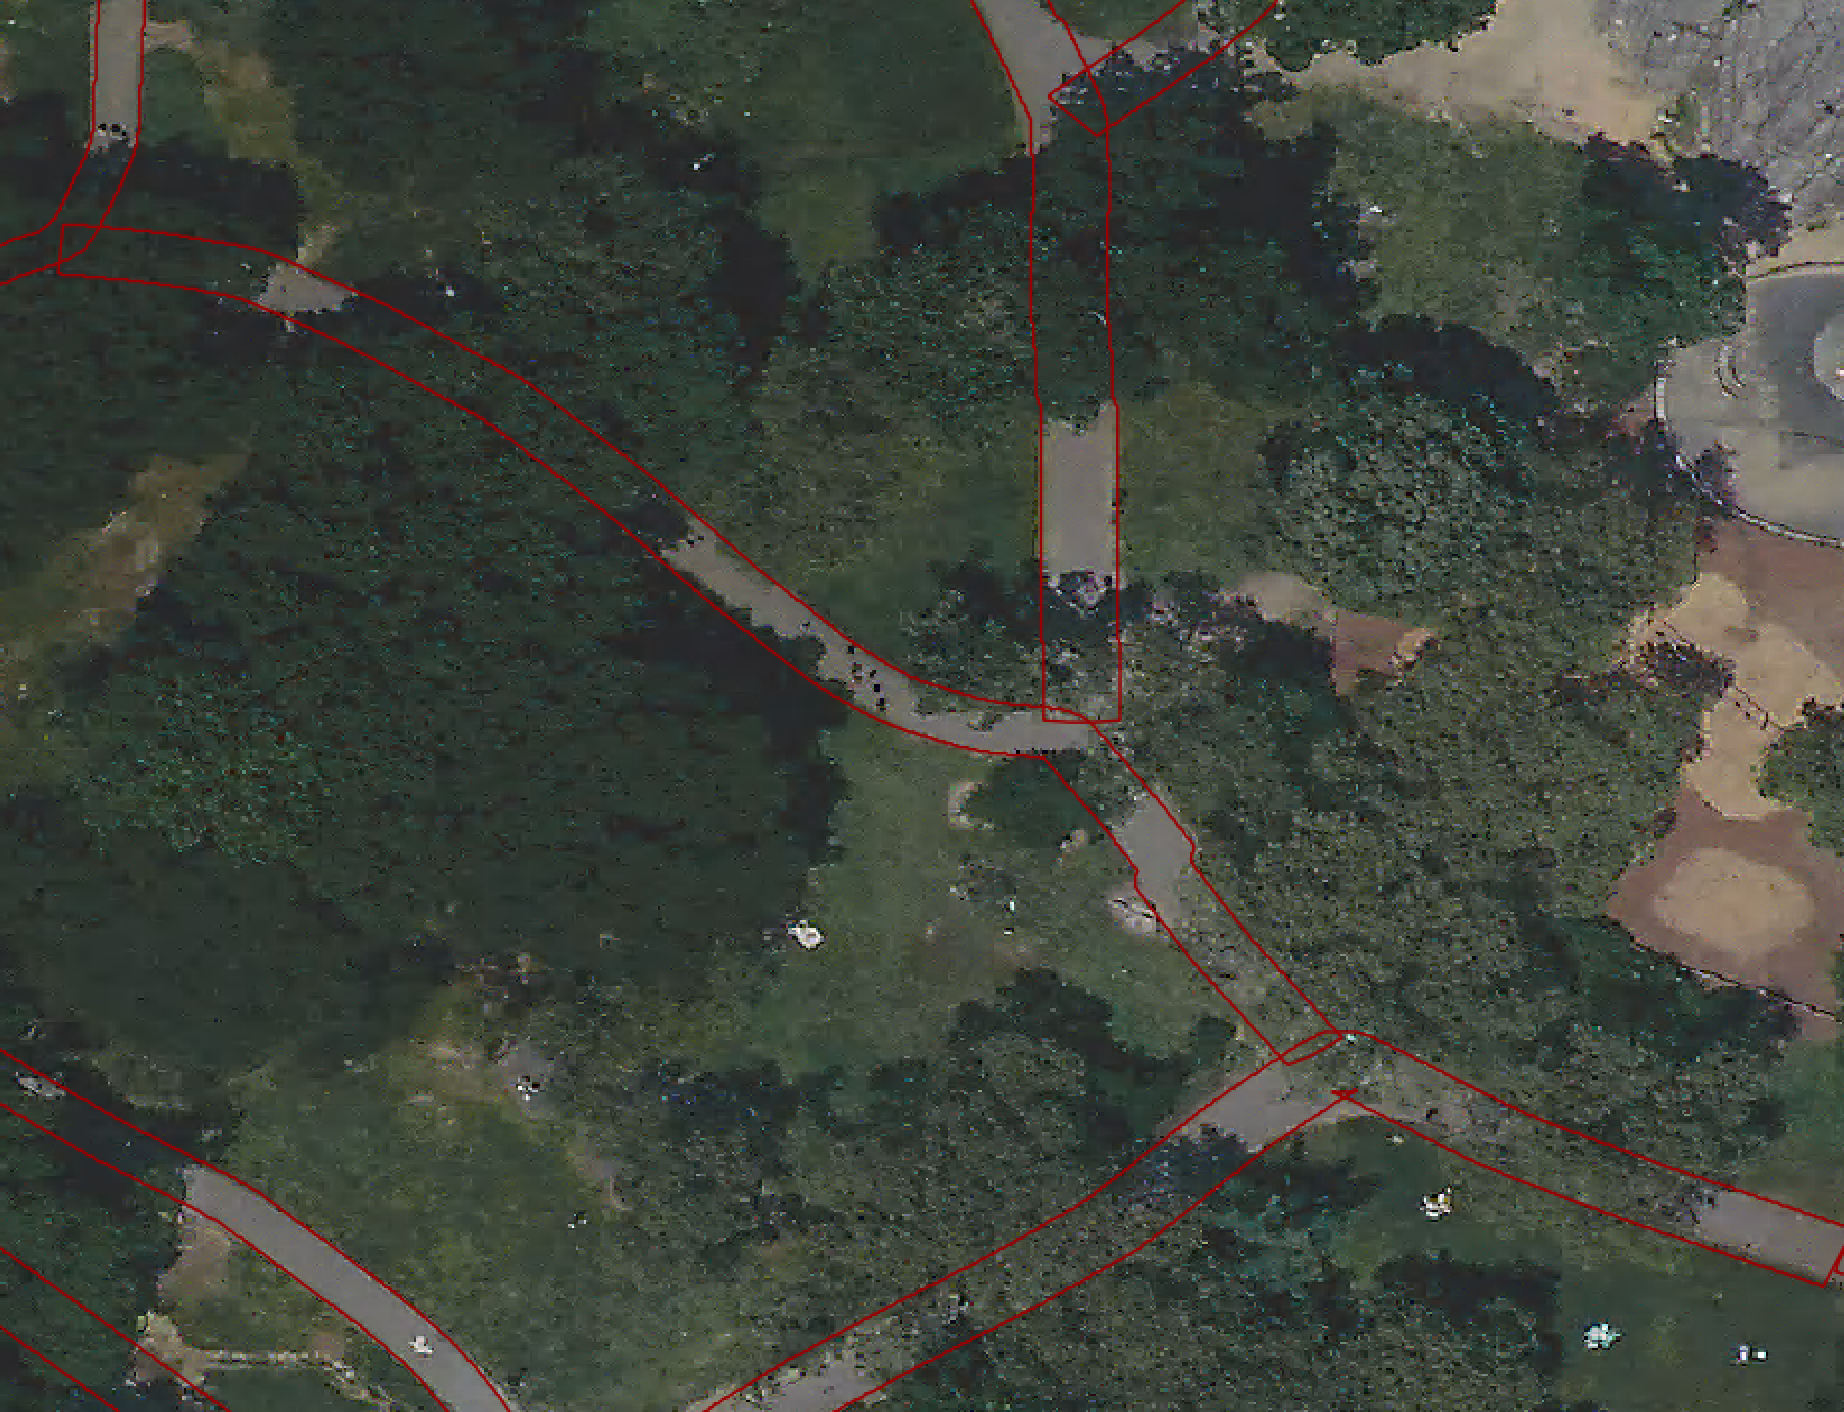
\includegraphics[width=\textwidth]{Figures/ny1.png}
    \caption[Sample Sidewalk 4]{Demonstration on sample sidewalks with our approach. We use New York area that include more complex sidewalks. Our approach is able to separate tree shadows and obstacles. It also has a decent performance on predicating boundaries on partial sidewalks that are fully covered by tree leaves.}
    \label{fig:ny1}
\end{figure}

\begin{figure}
    \centering
    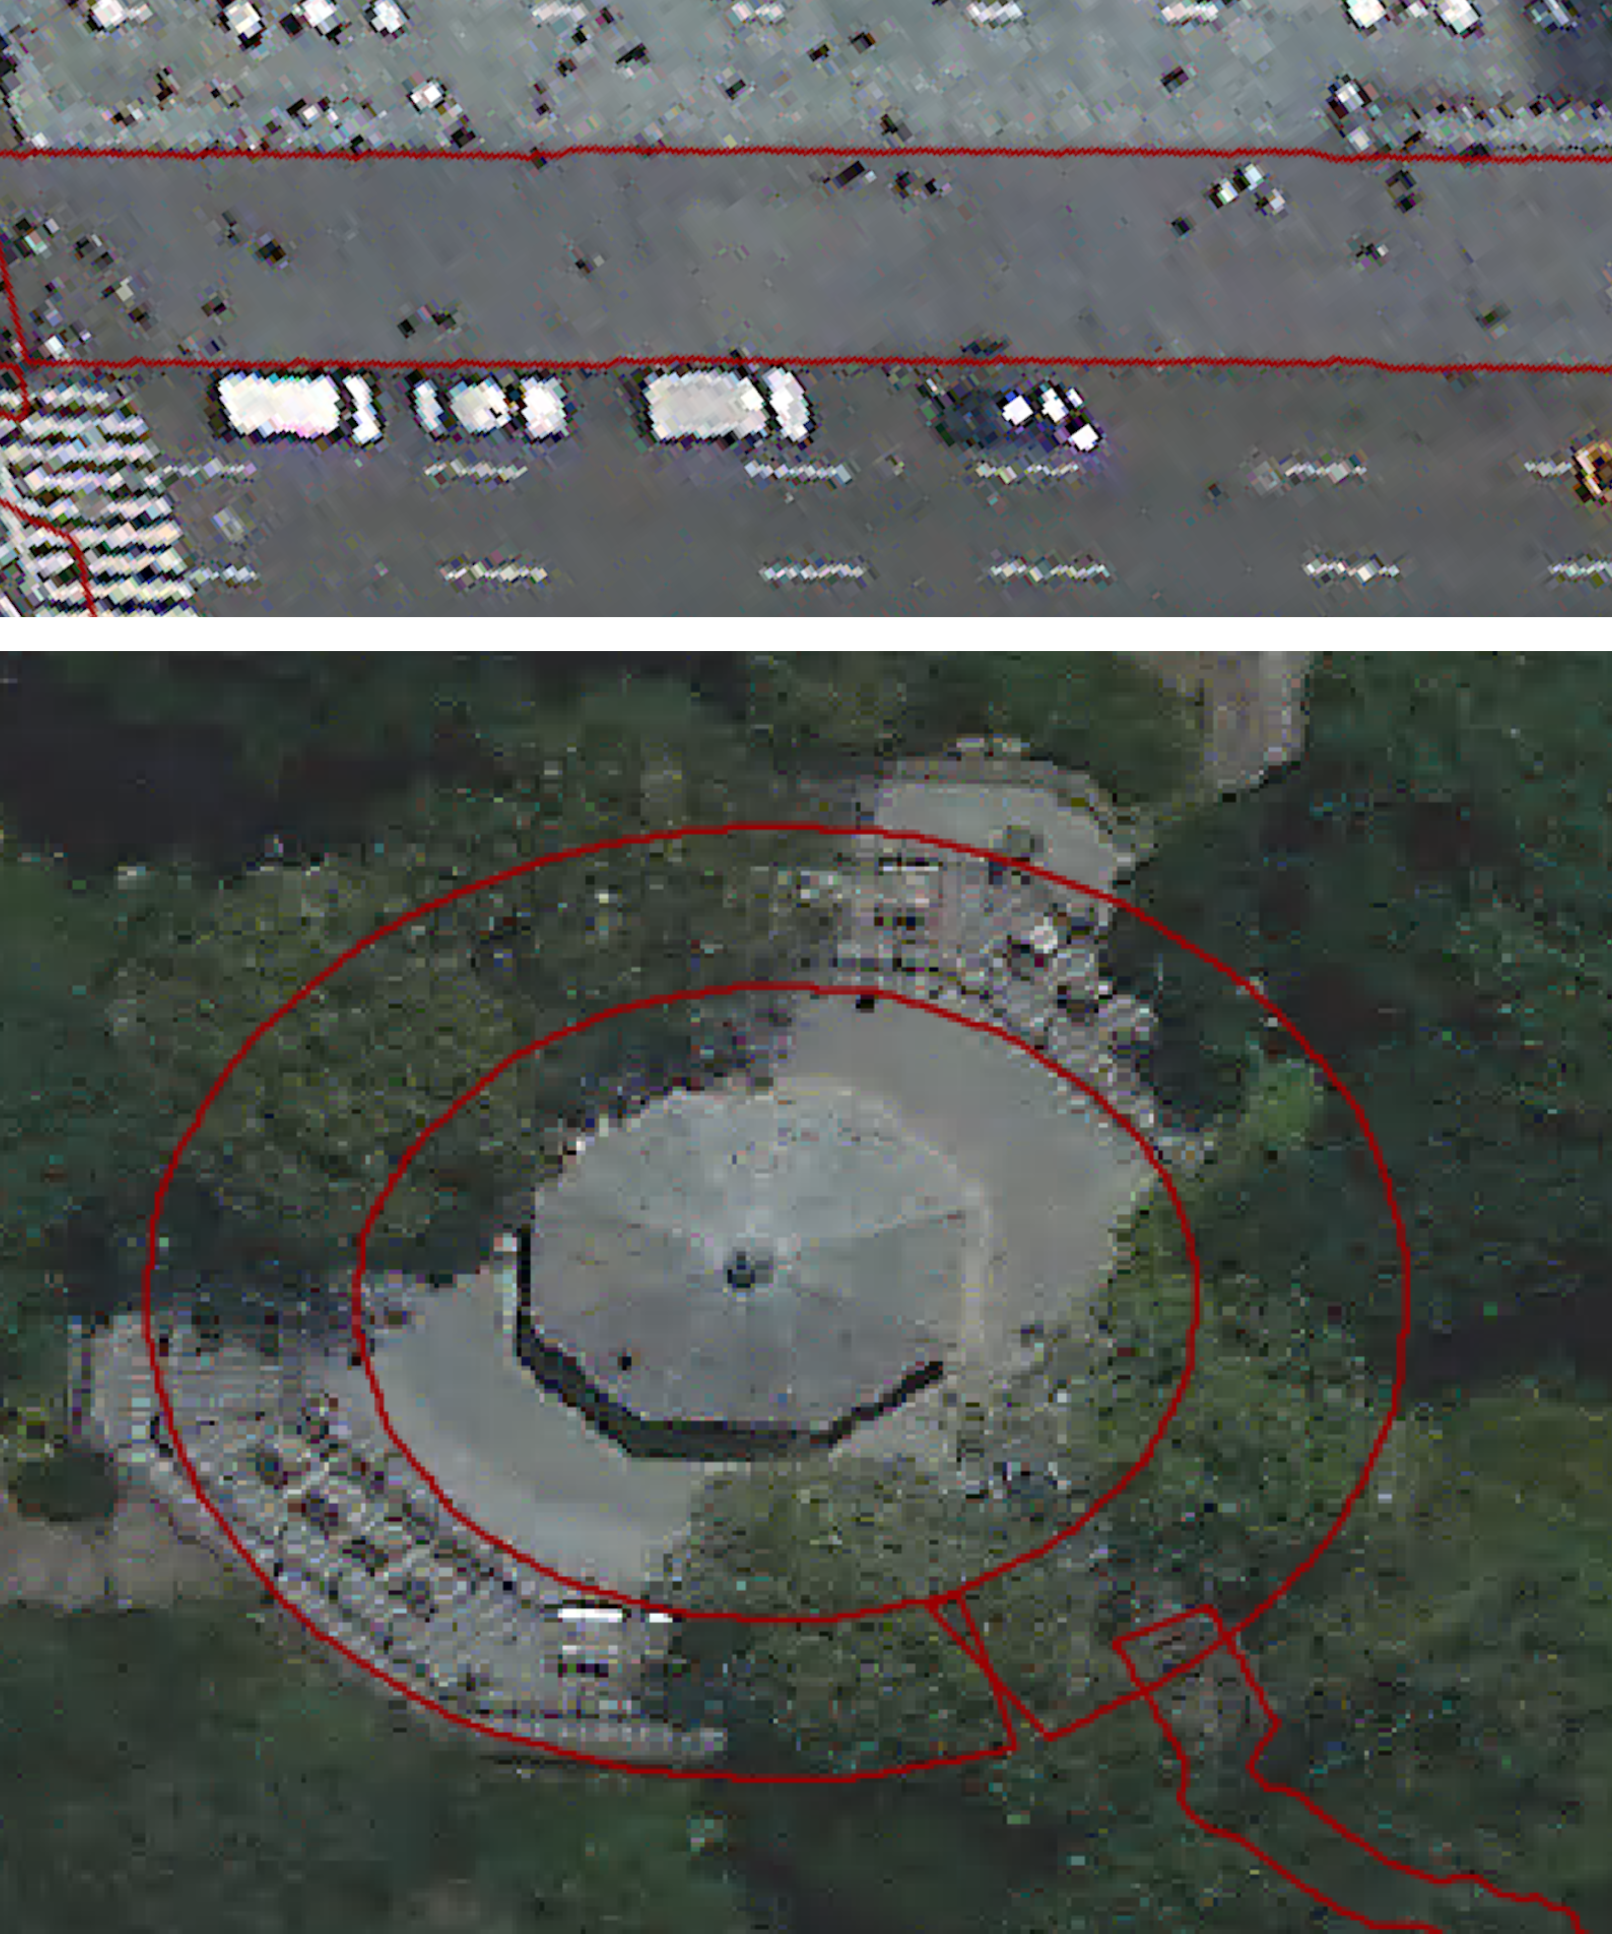
\includegraphics[width=\textwidth]{Figures/ny2.png}
    \caption[Sample Sidewalk 5]{Demonstration on sample sidewalks with our approach. We use sidewalks that are random selected from New York area. Row 1 shows a thicker sidewalk that camouflage with adjacent road and street. Row 2 shows complex sidewalk texture with irregular shape.}
    \label{fig:ny2}
\end{figure}

\begin{figure}
    \centering
    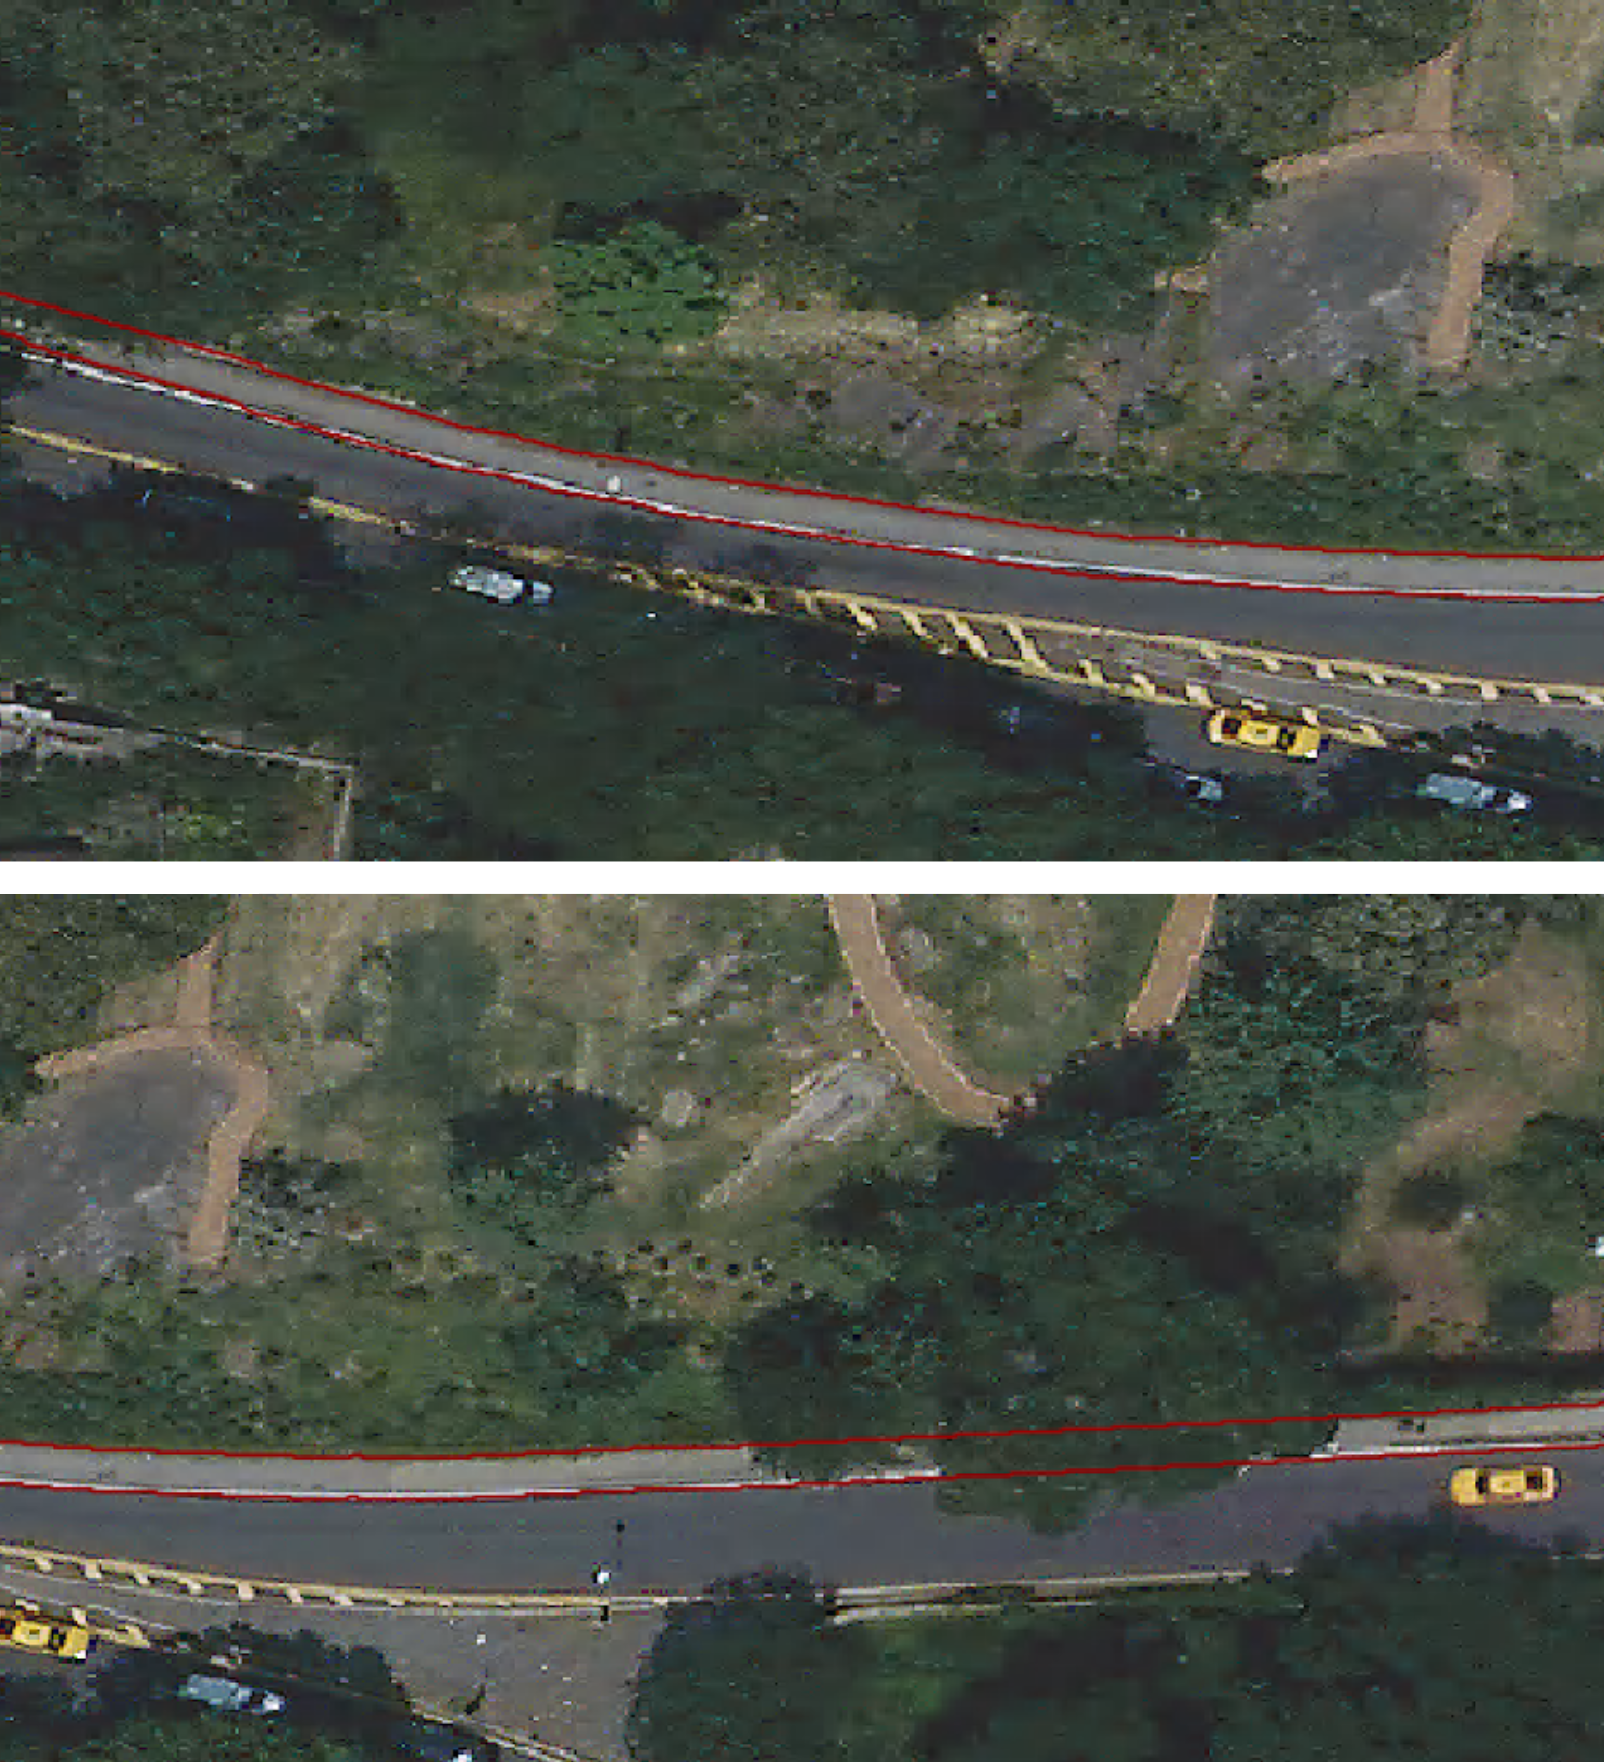
\includegraphics[width=\textwidth]{Figures/ny3.png}
    \caption[Sample Sidewalk 6]{Demonstration on sample sidewalks with our approach. It shows a continues site but we separate it due to it's length. Our approach did recognized the sidewalk part under the tree top and predict it's precise boundaries.}
    \label{fig:ny3}
\end{figure}


\chapter{Conclusion}
In this thesis defense, we have investigated a dynamic programming approach to segment sidewalk as a ribbon-like feature. We believe the preliminary result from our hypothesis is decent. During thesis progress, we gain the knowledge on important backgrounds and we study other feature extraction methods. Also, we develop a fully working dynamic programming algorithm with penalty control function to achieve better performance.

\section{Summary}
Chapter 2 introduces a few important background knowledge for better understanding of this thesis defense. We go through \ac{VHR}, \ac{OSM}\cite{OpenStreetMap}, \ac{CRF}\cite{MAL-013}, \ac{GMM}\cite{sridharan2014gaussian} and \ac{DP}\cite{bellman2013dynamic} to understand the basic of our approach.   

Chapter 3 shows the experiments that we researched on similar topics on feature extraction from image and sidewalk segmentation method. Mainly, we compared with segmentation tools, such as grabcut\cite{Rother2004-ou}, slic\cite{Achanta:149300}, and active contours \cite{Kass88snakes:active}. These three methods had fairly performance on segmentation sidewalk feature from input. Different but related methods were also applied such as road extraction\cite{road_detect}.

Chapter 4 carefully considers a hypothesis for our dynamic programming approach. Introduce the idea to segment ribbon-like feature by converting it's original shape into ribbon-shape. Also we developed a mathematics solution and a lattice representation of the problem, to help us build our dynamic programming solution better in the chapter 6.

Chapter 5 shows the publication that submitted base on our approach. We reproduce the hypothesis with more detail demonstration for the approach and involved algorithms. 

Chapter 6 brings a four-step approach in order to generate precise boundaries for given sidewalk, locate sidewalk geometric information, generating ribbon-image, applying density estimation function and applying our dynamic program algorithm with width control. Output from the approach would be compared from the other methods.

\section{Failure Cases}

We produce some failure cases to show what we need to improve for the future work. 

\begin{enumerate}
    \item Miss matching data set: Figure \ref{fig:oxford_fail_1} shows the failure case when the input map data and the trajectory data not match. The map data is older than the trajectory data, so the boundaries we generated is not yet existed on the map. Since the road structures changes over time, it's possible to get the data set in different time stamp. 
    \item Irregular Intersections: Figure \ref{fig:oxford_fail_2} shows the failure case when process irregular shape intersections. Our approach is able to generate the boundaries when the sidewalk is able to reshape into ribbon-image. Such as in figure \ref{fig:oxford_fail_2}, it's not yet able to produce the sidewalk boundaries with irregular shape intersection.
    \item Fully blocked sidewalk: \figref{fig:ny_fail_1} shows sample of sidewalks that fully blocked by obstacles, tree crown in our case. Base on the initial trajectory we find from open source, there must be a sidewalk under the tree crown. We count this as 'failure' cases since it's impossible for us to determine the accuracy for our result. 
\end{enumerate}

\begin{figure}
    \centering
    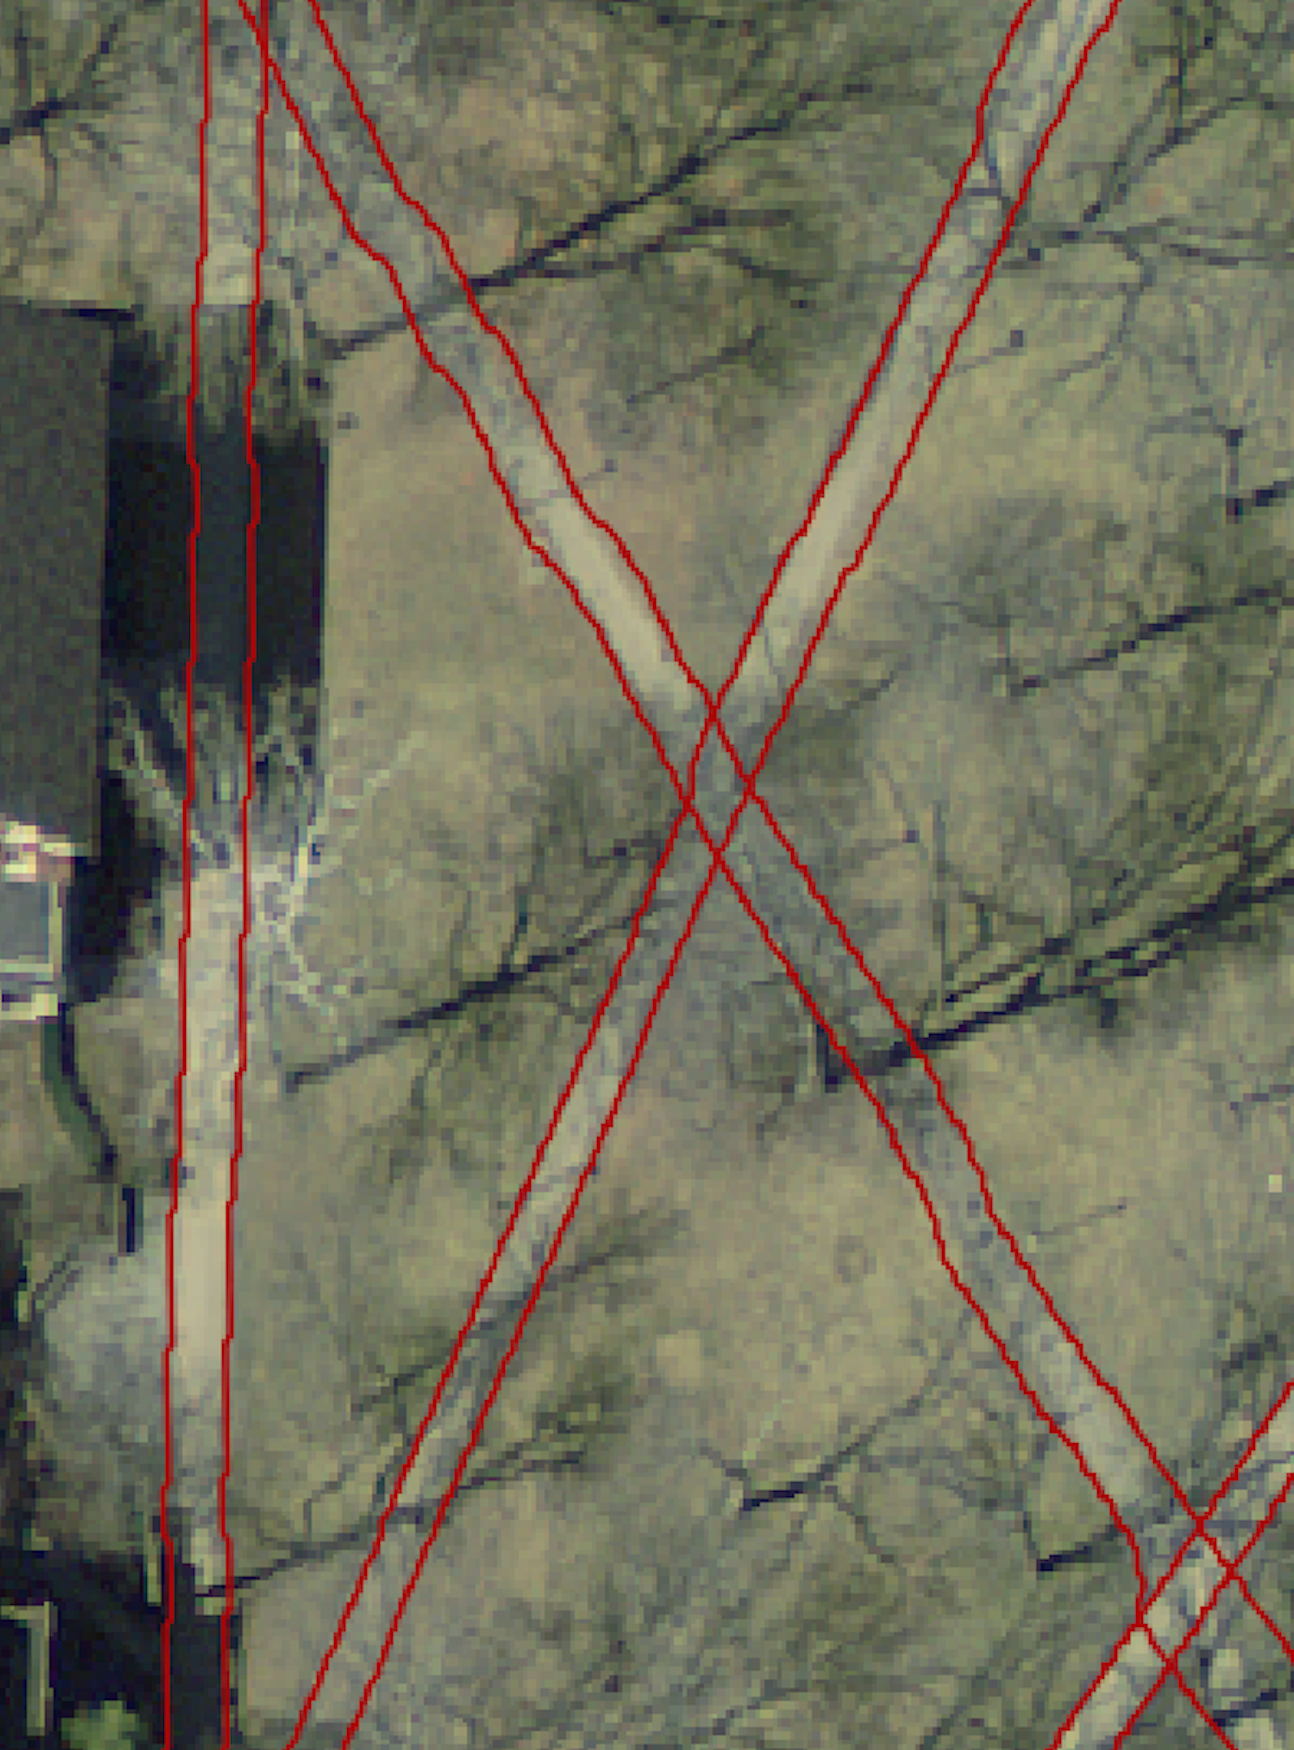
\includegraphics[width=0.83\textwidth]{Figures/oxford_fail_1.png}
    \caption[Failure Case 1]{Demonstration on failure cases. Due to the fact that road structures may change overtime. It's possible to produce the output with the input map and the initial trajectory within different time stamp. Sample figure shows our approach produce 'incorrect' sidewalk boundaries because the map data is older than the trajectory so we are producing the sidewalk that were not built yet.}
    \label{fig:oxford_fail_1}
\end{figure} 

\begin{figure}
    \centering
    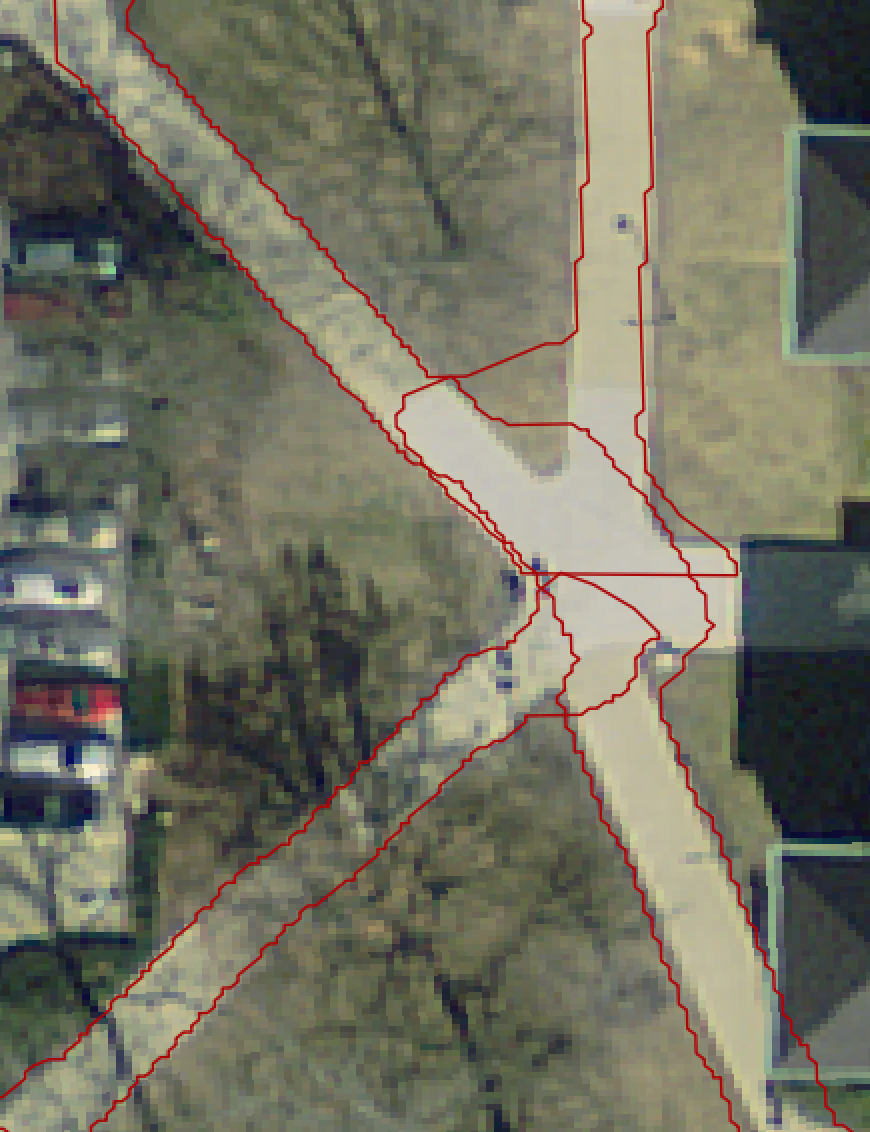
\includegraphics[width=0.9\textwidth]{Figures/oxford_fail_2.png}
    \caption[Failure Case 2]{Demonstration on failure cases. Our approach was developed to produce boundaries for single sidewalk, and it's not yet able to process intersection with irregular shape.}
    \label{fig:oxford_fail_2}
\end{figure} 

\begin{figure}
    \centering
    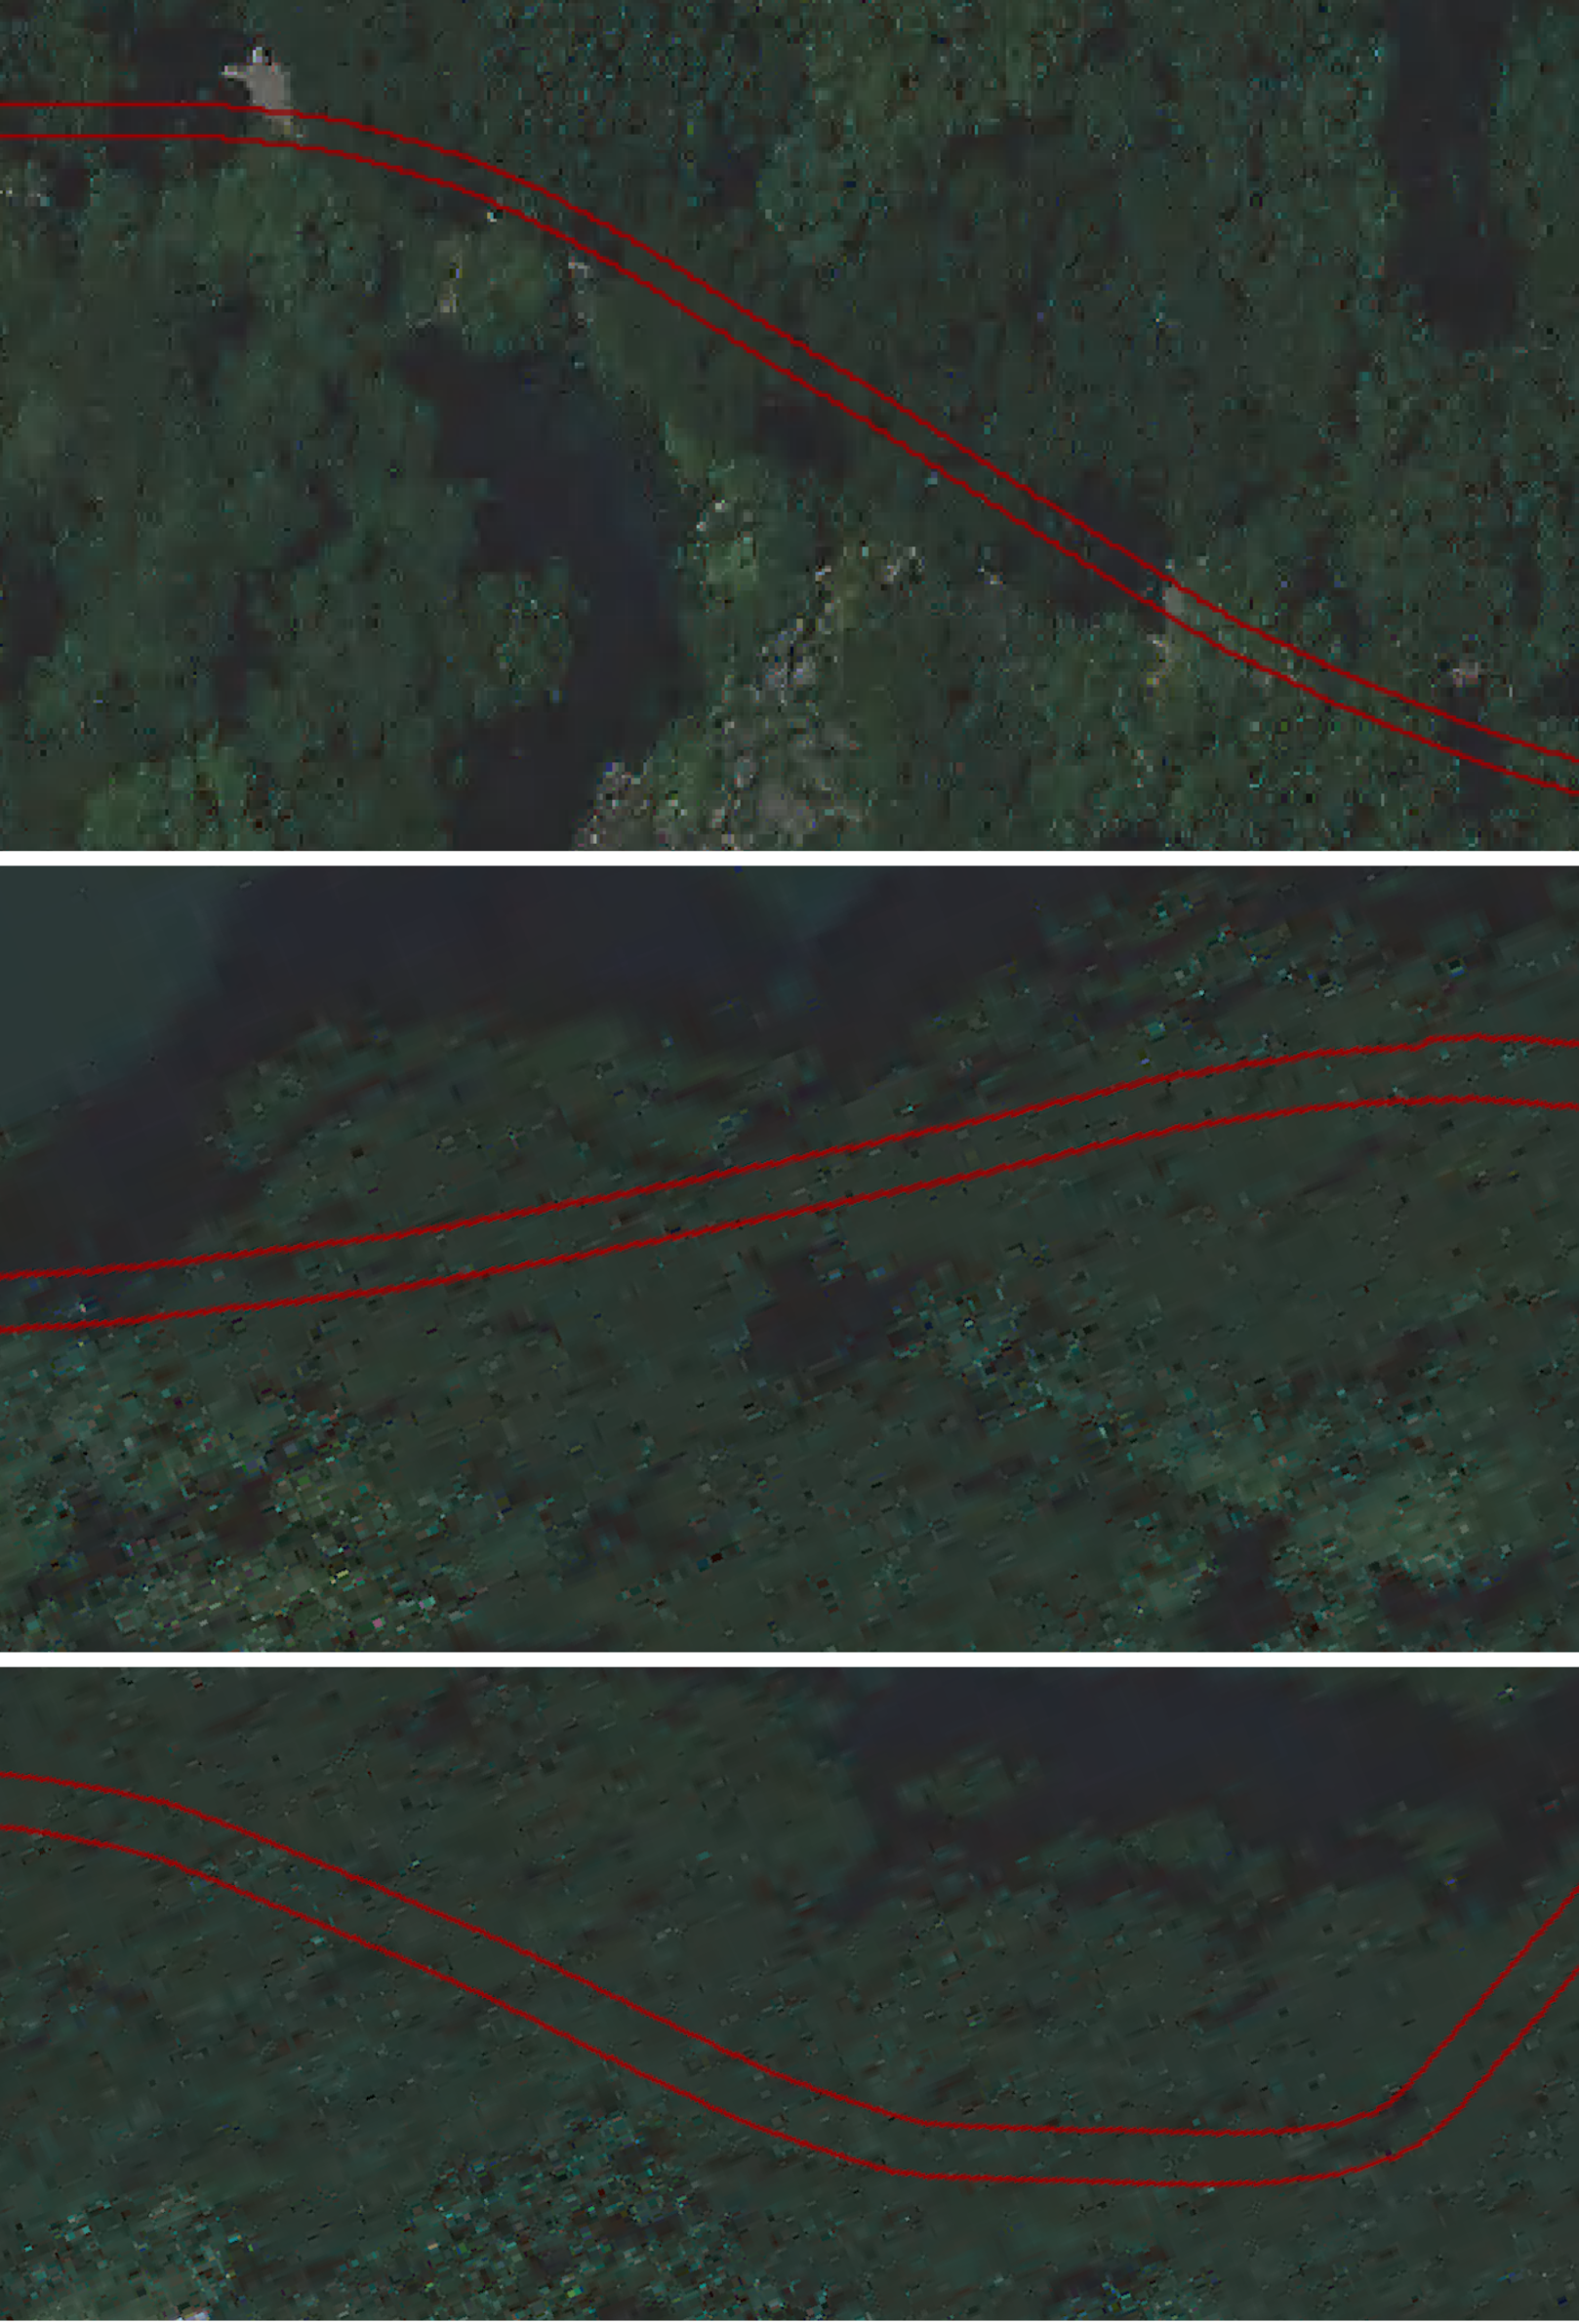
\includegraphics[width=0.8\textwidth]{Figures/ny_failcase.png}
    \caption[Failure Case 3]{Demonstration on failure cases. Our approach is not able to determine the sidewalk boundaries that's completely blocked by obstacles. The result is base on the average of sidewalks width but it's impossible for us to compare the prediction with accurate result.}
    \label{fig:ny_fail_1}
\end{figure} 

\section{Future Work}

There's couple more ideas we would like to attempt.

\begin{enumerate}
    \item To simplify the process, we would like to generate the sidewalk with just latitudes and longitudes.
    
    we can use the latitudes and longitudes data to locate a part of a map via Overpass Turbo \cite{overpass_turbo}, it supports features such as sidewalks geometric location since it's connecting with the database from \ac{OSM} \cite{OpenStreetMap}. Also, with the input latitudes and longitudes data, we can extract the map with given range from Google map or other open map source. Then just simply pass in both data set with our approach to generate whole sidewalk information for the whole site. 
    
    \item We'll give hypothesis to process the intersection area. By identify the point that is overlapped as intersection part (same node in multiple ways), we connect nodes on each way that are adjacent to the point. By extend each path a little bit more into the adjacent path to finish the intersection.
    
\end{enumerate}

% \appendix
% %\chapter{Source Code for XXX}
% We show the source code for XXXX
% \include{Appendices/A2}
% \include{Appendices/A3}
% \include{Appendices/A4}

\backmatter

\bibliographystyle{unsrt}
\addcontentsline{toc}{chapter}{References}
\bibliography{Thesis}
\end{document}